%\documentclass[11pt]{article}

%\documentclass[a4paper,UKenglish,cleveref, autoref,]{lipics-v2019}
%\documentclass[a4paper,english,cleveref, autoref]{lipics-v2019}

%\nolinenumbers
\documentclass[11pt,letter]{article}

\usepackage{amsmath,amssymb,amsthm}
\usepackage{thmtools}
\usepackage{thm-restate}
%\usepackage{authblk}
%%Changed 2cm ==> 2in -H
\usepackage[margin=1in]{geometry}
\usepackage[utf8]{inputenc}
\usepackage{booktabs}
%\declaretheorem{theorem}
\usepackage{amsmath}
\usepackage[colorlinks=true,linkcolor=red,citecolor=blue]{hyperref}
\usepackage{amssymb}
\usepackage{tikz}
\usetikzlibrary{topaths,calc}
%\usetikzlibrary{decorations.pathreplacing,calligraphy}
\usepackage{thm-restate,thmtools}
\usepackage{mathtools}
\usepackage{amsthm}
\usepackage{dsfont}
\usepackage{color}
\usepackage{amsmath}
\usepackage{amsfonts}
\usepackage{amssymb}
\usepackage{bbm}
\usepackage{relsize}
\usepackage{enumitem}
\usepackage[procnumbered, linesnumbered,algoruled]{algorithm2e}
%\usepackage[compact]{titlesec}
\usepackage{lineno}
%\linenumbers
%\usepackage{hyperref}
%\usepackage{cleveref}
%\usepackage{booktabs}
\usepackage{array}



\usepackage[nameinlink]{cleveref}
%\usepackage{enumitem}
%\linenumbers
%\renewcommand{\baselinestretch}{1.1}
	\def\claimproof{\proof}
\def\endclaimproof{\hfill$\square$\\}
\renewcommand\qedsymbol{$\blacksquare$}
\newcommand{\pp}{$\Pi$-matroid}
\newcommand{\negA}{\vspace{-0.05in}}
\newcommand{\negB}{\vspace{-0.1in}}
\newcommand{\negC}{\vspace{-0.18in}}
\newcommand{\posA}{\vspace{0.08in}}
\newcommand{\mysection}[1]{\negC\section{#1}\negA}
\newcommand{\mysubsection}[1]{\negB\subsection{#1}\negA}
\newcommand{\mysubsubsection}[1]{\negB\subsubsection{#1}\negA}
\newcommand{\myparagraph}[1]{\par\smallskip\par\noindent{\bf{}#1:~}}
\newcommand{\ceil}[1]{{\left\lceil#1  \right\rceil}}
\newcommand{\comment}[1]{}
\newcommand\numberthis{\addtocounter{equation}{1}\tag{\theequation}}

\newcommand{\mm}{M_{n,k,\alpha}(\Pi)}
% \newcommand{\comment}[1]{}
\newcommand{\opt}{\textnormal{opt}}
\newcommand{\bases}{\textnormal{bases}}
\newcommand{\IS}{\textnormal{IS}}
\newcommand{\cA}{{\mathcal{A}}}
\newcommand{\cB}{{\mathcal{B}}}
\newcommand{\cQ}{{\mathcal{Q}}}
\newcommand{\cG}{{\mathcal{G}}}
\newcommand{\cI}{{\mathcal{I}}}
\newcommand{\ci}{{\mathcal{I}}}
\newcommand{\cD}{{\mathcal{D}}}
\newcommand{\cm}{{\mathcal{M}}}
\newcommand{\ck}{{\mathcal{K}}}
\newcommand{\cF}{{\mathcal{F}}}
\newcommand{\cJ}{{\mathcal{J}}}
\newcommand{\cj}{{\mathcal{J}}}
\newcommand{\cIR}{{\mathcal{I}_R}}
\newcommand{\po}{\textnormal{poly}}
\newcommand{\co}{{\mathcal{O}}}
\newcommand{\fs}{f_{\textnormal{SAT}}}
\newcommand{\io}{|I|^{O(1)}}
\def \NN   {{\cal N}}
\def \CC   {{\cal C}}

\newcommand{\cP}{{\mathcal{P}}}
\newcommand{\cC}{{\mathcal{C}}}
\newcommand{\bx}{{\bar{x}}}
\newcommand{\by}{{\bar{y}}}
\newcommand{\bz}{{\bar{z}}}
\newcommand{\bc}{{\bar{c}}}
\newcommand{\OPT}{\textnormal{OPT}}
\newcommand{\greedy}{\textsc{Greedy}}
\newcommand{\greedyplus}{\textsc{Greedy+Singleton}}
\newcommand{\enum}{\textsc{EnumGreedy}}
\newcommand{\eps}{{\varepsilon}}
\newcommand{\aeps}{{d}}
\newcommand{\E}{{\mathbb{E}}}
\newcommand{\floor}[1]{\left\lfloor #1 \right\rfloor}
\DeclareMathOperator*{\argmax}{arg\,max}
\DeclareMathOperator*{\argmin}{arg\,min}
\newcommand{\klf}{{\varphi}}


%\newcommand{\problem}[2]{
%	
%	\noindent
%	\begin{tabular}{ p{0.8in}  p{5.4 in}  }
%	\\
%	multicolumn{2}{c}{#1} \\
%	\hline
%	#2\\
%	\hline
%	\\
%\end{tabular}
%}
%\newcommand{\problem}[2]{
%	\noindent
%	\begin{tabular}{ | p{0.8in} | p{5.4in} | }
%		\hline
%		\multicolumn{2}{|c|}{#1} \\
%		\hline
%		#2\\
%		\hline
%	\end{tabular}
%}


\newcommand{\problem}[2]{
	\noindent
	\begin{tabular}{ p{0.8in} p{5.4in} }
		\\
		\hline
		\multicolumn{2}{c}{#1} \\
		\hline
		#2\\
		\hline
		\\
	\end{tabular}
}


\newcommand{\BM}{\textnormal{BM}}



\newtheorem{lemma}{Lemma}[section]
%\newtheorem{thm}[lemma]{Theorem}
\newtheorem{prop}[lemma]{Proposition}
\newtheorem{assm}[lemma]{Assumption}
\newtheorem{lem}[lemma]{Lemma}
\newtheorem{obs}[lemma]{Observation}
\newtheorem{cor}[lemma]{Corollary}
\newtheorem{definition}[lemma]{Definition}
\newtheorem{theorem}[lemma]{Theorem}
\newtheorem{proposition}[lemma]{Proposition}
\newtheorem{observation}[lemma]{Observation}
\newtheorem{claim}[lemma]{Claim}
\crefname{claim}{claim}{claims}

\newtheorem{example}[lemma]{Example}
\newtheorem{defn}[lemma]{Definition}
\newcommand{\ariel}[1]{{\color{blue} (Ariel :#1)}}
\newcommand{\ilan}[1]{{\color{blue} Ilan: \color{magenta}#1}}
%\newcommand{\danny}[1]{{\color{violet} Danny :\color{magenta}#1}}
\def \II   {{\mathcal I}}
\newcommand{\one}{\mathbbm{1}}
	\crefname{claim}{claim}{claims}
		\crefname{cor}{corollary}{corollaries}
\begin{document}

	
	
	%\setcost{\textwidth}{6.5in}
	%\setcost{\textheight}{8.7in} %was 9in
	%\setcost{\oddsidemargin}{0in}
	%\setcost{\evensidemargin}{0in}
	%\setcost{\topmargin}{0.0in}
	%\setcost{\headheight}{0in}
	%\setcost{\headsep}{0.4in}
	%\setcost{\footskip}{0.4in}
	
	%\begin{titlepage}
	%	\begin{titlepage}
		\title{
			  Lower Bounds for Matroid Optimization Problems with \\ a Linear Constraint
		}
	%		\author{Anonymous }
		
		\author{Ilan Doron-Arad\thanks{Computer Science Department, 
				Technion, Haifa, Israel. \texttt{idoron-arad@cs.technion.ac.il}}
			\and
			Ariel Kulik\thanks{CISPA Helmholtz Center for Information Security, Saarland Informatics Campus, Germany. \texttt{ariel.kulik@cispa.de}} 
			\and
			Hadas Shachnai\thanks{Computer Science Department, 
				Technion, Haifa, Israel. \texttt{hadas@cs.technion.ac.il}}
		}
%				
		\maketitle
		\thispagestyle{empty}
		
		\begin{abstract}
			
We study a family of {\em matroid optimization problems with a linear constraint} (MOL). 
In these problems, we seek a subset of elements which optimizes (i.e., maximizes or minimizes) a linear objective function subject to (i) a matroid independent set, or a matroid basis constraint, (ii) additional linear constraint. A notable 
member in this family is {\sc budgeted matroid independent set (BM)}, which  can be viewed as classic $0/1${\sc-knapsack} with a matroid constraint. While special cases of BM, such as  {\sc knapsack with cardinality constraint} and {\sc multiple-choice knapsack}, admit a {\em fully polynomial-time approximation scheme} (Fully PTAS), the best known result for BM on a general matroid is an {\em Efficient} PTAS. Prior to this work, the existence of a Fully PTAS for BM, and more generally, for any problem in the  family of MOL problems, 
has been open.

In this paper, we answer this question negatively by showing that none of the (non-trivial) problems in this family admits a Fully PTAS. This resolves the complexity status of several well studied problems. Our main result is obtained by showing first that {\sc exact weight matroid basis (EMB)} does not admit a pseudo-polynomial time algorithm. This distinguishes EMB from the special cases of $k$-{\sc subset sum} and EMB on a linear matroid, which are solvable in pseudo-polynomial time.
We then obtain unconditional hardness results for the family of MOL 
problems in the oracle model (even if randomization is allowed), and show that the same results hold when the matroids are encoded as part of the input, assuming $\textnormal{P} \neq \textnormal{NP}$. For the hardness proof of EMB, we introduce the $\Pi$-{\em matroid} family. This intricate subclass of matroids, which exploits the interaction 
between a weight function and the matroid constraint, may find use in tackling other matroid optimization problems.


		\end{abstract}
		
		\newpage

		\setcounter{page}{1}
		
			\section{Introduction}
	\label{sec:intro}
	
	Matroids are simple combinatorial structures, providing
	a unified abstraction for independence systems such as linear independence in a vector space, or cycle-free subsets of edges in a given graph. A {\em matroid} is a set system $(E, \cI)$, where $E$ is a finite set and $\cI \subseteq 2^E$ are the {\em independent sets (IS)} such that $(i)$ $\emptyset \in \cI$, $(ii)$ for all $A \in \cI$ and $B \subseteq A$ it holds that $B \in \cI$, and $(iii)$ for all $A,B \in \cI$ where $|A| > |B|$, there is $e \in A \setminus B$ such that $B \cup \{e\} \in \cI$.\footnote{Properties $(ii)$ and $(iii)$ are known as {\em hereditary property},
		and  {\em exchange property}.}
	
	While serving as a generic abstraction for numerous applications, matroids possess useful combinatorial properties that allow the development of efficient algorithms. 
	These algorithms include such canonical results as the classic greedy approach for finding a maximum weight independent set of a matroid (see, e.g., \cite{CLRS22}), Edmond's algorithm for matroid partitioning \cite{edmonds1965minimum}, and Lawler's algorithm for matroid intersection \cite{La75}. In all of the above, polynomial running time is enabled due to the structure of the problem $-$ a single objective function with a matroid constraint. However, in many natural applications, there is an added {\em linear} constraint. 
	
	Consider, for example, the problem of finding a maximum independent set in a matroid subject to a budget constraint. Formally, we are given 
	a set of elements $E$, a membership oracle for a collection of independent sets $\II \subseteq 2^{E}$ of a matroid $(E, \II)$, %where $(E, \II)$ is a matroid, 
	a budget $L>0$, a weight function~$w:E\to \mathbb{R}_{\geq 0}$, and a value function $v:E\rightarrow \mathbb{R}_{\geq 0}$. A {\em solution} for the problem is an independent set $S \in \II$ of total weight at most $L$, i.e., $w(S) \leq L$.\footnote{For every set $X$, a function $f:X \rightarrow \mathbb{R}_{\geq 0}$ and $Y \subseteq X$ we define $f(Y) = \sum_{e \in Y} f(e)$.} The {\em value} of a solution $S$ is given by $v(S)$,
	and the objective is to find a solution of maximum value. This problem, known as {\sc budgeted matroid independent set (BM)}, is a generalization of the classic $0/1${\sc-knapsack}, which is NP-hard
	and therefore unlikely to admit an exact polynomial-time algorithm. Thus, obtaining efficient approximations has been a main focus in the study of BM.

	
 For an instance $I$ of an optimization problem $\cG$, let $\OPT_{\cG}(I)$ be the value of an optimal solution for $I$. For some $\rho \geq 1$, a {\em $\rho$-approximate solution} $S$ for $I$ is a solution of value $v \geq \frac{\OPT_{\cG}(I)}{\rho}$ ($v \leq \rho \cdot \OPT_{\cG}(I)$) if $\cG$ is a maximization (minimization) problem. 
 We say that $\cA$ is a {\em randomized $\rho$-approximation algorithm} for $\cG$ if,
given an instance $I$ of $\cG$, $\cA$
returns with probability at least $\frac{1}{2}$ a $\rho$-approximate solution for $I$ $-$ if a solution exists. If no solution exists $-$ $\cA$ returns that $I$ does not have a solution.
	

	
	
	
	Let $|I|$ be the encoding size of an instance~$I$ of a problem $\cG$. 
	A (randomized) {\em polynomial-time approximation scheme} (PTAS)
	for $\cG$ is a family of algorithms $(A_{\eps})_{\eps>0}$ such that, for any $\eps>0$, $A_{\eps}$ is a (randomized) polynomial-time $(1+ \eps)$-approximation algorithm for $\cG$. 
	A (randomized) {\em Efficient PTAS} (EPTAS) is a (randomized) PTAS $(A_{\eps})_{\eps>0}$ with running time of the form $f\left(\frac{1}{\eps}\right) \cdot |I|^{O(1)}$, where $f$ is an arbitrary computable function. %We say that 	
	The strong dependence of run-times on the error parameter, $\eps > 0$, often renders the above schemes highly impractical. This led to the study of the following more desirable class of schemes. A (randomized) approximation scheme 
	$(A_{\eps})_{\eps>0}$ is a (randomized) {\em Fully PTAS} (FPTAS) if the running time of $A_{\eps}$ is of the form $ {\left(\frac{|I|}{\eps}\right)}^{O(1)}$.\footnote{To better distinguish between EPTAS and FPTAS, we use throughout the paper Efficient PTAS and Fully PTAS.}
	
In the past decades, BM was shown to admit a PTAS~\cite{BBGS11,CVZ11,GZ10}, and more recently an Efficient PTAS \cite{DKS23,DKS23b}. As the special case of
%$BM generalizes 
$0/1${\sc-knapsack} admits a Fully PTAS, it is natural to explore the existence of a Fully PTAS for BM. There are known Fully PTASs  for BM on restricted families of matroids. This includes {\sc knapsack with a cardinality constraint}~\cite{caprara2000approximation}, 
{\sc multiple-choice knapsack}~\cite{La79}, and {\sc BM with laminar matroid constraint} \cite{DKS23c}. However, the question of whether BM admits a Fully PTAS on general matroids remained open. 

In this paper, we resolve this question negatively for BM and other fundamental matroid optimization problems with a linear constraint. 

\subsection{Our Results}

For a matroid $\cm = (E,\cI)$ we define $\IS(\cm) = \cI$ and $\bases(\cm) = \{S \in \cI~|~|S| = \textsf{rank}(\cm)\}$, where $\textsf{rank}(\cm) = \max_{T \in \cI} |T|$ is the {\em rank} of $\cm$, i.e., the maximum cardinality of an independent set. We study a family of {\em matroid optimization problems with a linear constraint} (MOL). Problems in this family are characterized by three parameters: 
\begin{enumerate}
\item[(i)]
%$(i)$ 
The optimization objective $\opt$ $-$ either the operator $``\max"$ or $``\min"$. 
\item[(ii)]
%$(ii)$ 
A {\em matroid feasibility constraint} $\cF$ $-$ either the independent sets of a matroid, or the set of {\em bases} of a matroid. The feasibility constraint is $\cF \in \{\IS,\bases\}$.
\item[(iii)]
%$(iii)$ 
A relation $\triangleleft$ $-$  realized by one of the relations $``\geq"$ or $``\leq"$. 
\end{enumerate}

Let $\cP = \{\max,\min\} \times \{\bases,\IS\} \times \{\leq ,\geq\}$ be the set of {\em parameters} for MOL problems. 
Based on the set of parameters $\cP$, we define for every triplet a problem
in the MOL family. For $P \in \cP$ where $P = \left(\opt,\cF,\triangleleft\right)$, define the $P$-{\sc matroid optimization with a linear constraint} ($P$-MOL) problem as follows. An instance is a tuple $I = (E,\cI,v,w,L)$ such that $\cm = (E,\cI)$ is a matroid, $v:E \rightarrow \mathbb{R}_{\geq 0}$ is the objective function, $w:E \rightarrow \mathbb{R}_{\geq 0}$ is a weight function, and $L \in \mathbb{R}_{\geq 0}$ is a {\em bound} for the linear constraint. 
A {\em solution} of $I$ is $S \subseteq E$ which satisfies the matroid feasibility constraint $S \in \cF(\cm)$ and the linear constraint $w(S) \triangleleft L$. The goal is to optimize (i.e., maximize or minimize) the value $v(S)$. Thus, we can formulate a P-MOL optimization problem as
\begin{equation}
\label{eq:0}
\opt~ v(S) \text{ s.t. } S \in \cF(\cm),~  w(S) \triangleleft L.
\end{equation} 



Observe that $(\max,\IS,\leq)$-MOL is the BM problem.
That is, given a BM instance (equivalently, $(\max,\IS,\leq)$-MOL instance) $I = (E,\cI,v,w,L)$, the goal is to find an independent set $S \in \cI$ of maximum total value $v(S)$ such that $w(S) \leq L$. Other notable examples for MOL problems are {\sc constrained minimum basis of a matroid} (CMB) \cite{HL04}, which can be cast as $(\min,\bases,\leq)$-MOL, and {\sc knapsack cover with matroid constraint} (KCM) \cite{CCNR13} formalized by $(\min,\IS,\geq)$-MOL.\footnote{CMB, KCM, and other MOL problems may not have a solution; however, we can decide in polynomial time if a solution exists, and our definition of approximation algorithms captures instances with no solution.}



We note that \eqref{eq:0} does not refer to the {\em representation} of the instance $I$. We consider two possible representations.
For any $P \in \cP$, in an instance $(E,\cI,v,w,L)$ of {\em oracle} $P$-MOL, the arguments
$E,v,w,L$ are given as the input, and the independent sets $\cI$ are accessed via a {\em membership oracle}, which determines whether a given set $S \subseteq E$ belongs to  $\cI$ in a single query. Thus, the independent sets are not considered in the encoding size of the instance. The term {\em running time} for problems involving oracles refers to the sum of the number of queries to the oracle and the number of basic operations. 
Previous works on MOL problems often consider membership oracles \cite{CVZ11,BBGS11,CCNR13,DKS23,DKS23b}. As hardness with oracles does not necessarily imply hardness in non-oracle models (see, e.g., \cite{canetti2004random,chang1994random}), in \Cref{sec:SAT} we show lower bounds for variants of MOL problems in which the independent sets are encoded as part of the input.   




Clearly, the problem $(\min,\IS,\leq)$-MOL is trivial since the empty set achieves the optimal objective value. 
However, for any other $P \in \cP$, solving the $P$-MOL problem is challenging.
The {\em non-trivial} MOL problems are all the MOL problems excluding $(\min,\IS,\leq)$-MOL. That is, $P$-MOL is non-trivial if $P\in \cQ$ where  $\cQ = \cP \setminus \{(\min,\IS,\leq)\}$.
%We consider the {\em non-trivial} MOL problems, whose parameters exclude the above triplet, i.e., $\cQ = \cP \setminus \{(\min,\IS,\leq)\}$.
 Observe that non-trivial MOL problems are NP-hard (e.g., $0/1${\sc-knapsack} is a special case of $(\max,\IS,\leq)$-MOL);
however, %several 
all previously studied MOL problems admit approximation schemes.




For certain special cases of MOL problems, e.g., BM with simple matroid constraints,
the existence of a Fully PTAS is known for decades \cite{Si79,caprara2000approximation}.
However, for MOL problems with arbitrary matroid constraints, the best known results are Efficient PTAS.  While matroids form an important generalization of well known basic
constraints,
% (cardinality constraint, linear independence in vector space, cycle-free subsets of edges in a graph, etc.), 
the complexity of the corresponding MOL problems remained open. Specifically, prior to this work, the existence of a MOL problem which does not admit a Fully PTAS was open.





Our main result is that none of the (non-trivial) 
oracle matroid optimization problem with a linear constraint admits 
a Fully PTAS, even if randomization is allowed. This unconditioned hardness result is established by deriving a lower bound on the minimum number of queries to the membership oracle. 
 \begin{restatable}{theorem}{thmMain}
	\label{thm:main}
	For every $P \in \cQ$ there is no randomized  \textnormal{Fully PTAS} for oracle $P$-\textnormal{MOL}. 
\end{restatable} 

\begin{table}[tbh]
	\centering
	\begin{tabular}{m{2.7in} m{1.4in} m{1.9in}}
		\toprule
		Problem & Previous Results & This Paper \\
		\midrule
		Budgeted Matroid Independent Set & Efficient PTAS \cite{DKS23} & {\bf No Fully PTAS} \\
		Budgeted Matroid Intersection & Efficient PTAS  \cite{DKS23b} & {\bf No Fully PTAS}  \\
		Constrained Minimum Basis of Matroid & Efficient PTAS  \cite{HL04} & {\bf No Fully PTAS} \\
		Knapsack Cover with a Matroid & PTAS \cite{CCNR13} & {\bf No Fully PTAS}  \\
		\bottomrule
	\end{tabular}
	\caption{Implications of our results for previously studied MOL problems. All of our bounds hold for randomized algorithms. }
	\label{tab:results}
\end{table}

\Cref{thm:main} conclusively distinguishes MOL problems with arbitrary matroids, such as BM, from special cases with simpler matroid constraints. Furthermore, it shows that existing Efficient PTAS \cite{HL04,DKS23,DKS23b} for MOL problems on general matroids are the best possible. Notable implications of our results are given in \Cref{tab:results}, and consequences of our lower bounds for a set of previously studied problems~\cite{ CGM92,HL04,BBGS11,CVZ11,GZ10,CCNR13,DKS23,DKS23b,doron2023budgeted}
are given in \Cref{sec:results}. By resolving the complexity status of MOL problems on general matroids, our results promote future research to design (or rule out) Fully PTAS for MOL problems on restricted matroid classes (see \Cref{sec:discussion}). 

To prove \Cref{thm:main}, we turn our attention to the following problem. %- a generalization of {\sc subset sum} with a matroid constraint. 
\begin{definition}
	\label{def:EMB}
	An instance of {\sc Exact Matroid Basis (EMB)}  is $I =  (E,\cI,c,T)$, where $(E,\cI)$ is a matroid, $c:E \rightarrow \mathbb{N}$ is a weight function, and $T \in \mathbb{N}$ is a target value. A {\em solution} is a basis $S$ of $(E,\cI)$ such that $c(S)=T$. The goal is to decide if there is a solution. 
\end{definition}
Similar to MOL problems, EMB does not specify the input. 
In an instance $(E,\cI,c,T)$ of {\sc oracle-EMB},
$E,c,T$ are explicitly given, and the independent sets $\cI$ are accessed via a membership oracle. An instance $I$ of a decision problem $\cD$
is a ``yes"-instance if the correct answer for $I$ is ``yes"; otherwise, $I$ is a ``no"-instance.
We say that $\cA$ is a {\em randomized algorithm} for a decision problem $\cD$ if,
% A {\em randomized algorithm} $\cA$ for a decision problem $\cD$ is an algorithm that,
 given a ``yes"-instance $I$ of $\cD$, $\cA$ returns ``yes"  with probability at least $\frac{1}{2}$; for a ``no"-instance, $\cA$ returns ``no" with probability $1$. The next result rules out a pseudo-polynomial time algorithm for oracle-EMB, thus distinguishing the problem from the special cases of $k$-{\sc subset sum} and EMB on linear matroids, which admit a pseudo-polynomial  time algorithm \cite{CGM92}. 
% We prove that the classic (randomized) pseudo-polynomial algorithm for oracle-EMB on {\em representable} (or, linear) matroids \cite{CGM92}, cannot be extended to general matroids.  

\begin{restatable}{theorem}{thmemb}
	\label{thm:emb}
	There is no randomized  algorithm  for {\sc oracle-EMB} that for any  \textnormal{oracle-EMB} instance $I =(E,\cI,c,T)$, where $n = |E|+1$ and  $m = c(E)+1$,  runs in time $ \left(n \cdot(T+2) \cdot m \right)^{O(1)}$. 
\end{restatable}

 

\subsection{Technical Contribution}
We derive our results by introducing $\Pi$-{\em matroids}.
This new family of matroids carefully exploits a simple weight function to define a matroid that successfully {\em hides} a specific property $\Pi$ within its independent sets (see \Cref{sec:technical}). Using $\Pi$-matroids, we define %the $\Pi$-{\em matroid problem} and prove its hardness; 
	oracle-EMB instances whose solutions must satisfy the property $\Pi$. This shows the unconditional hardness of oracle-EMB, as $\Pi$ can be discovered only via an exponential number of queries to the membership oracle. Our hardness results for MOL problems (as stated in \Cref{thm:main}) are derived via reduction from oracle-EMB.
	
	
		Despite the abundance of lower bounds for matroid problems~% , for example, the powerful bounds of Jensen and Korte~
		\cite{lovasz1978matroid,JK82,karp1985complexity,soto2014simple}, as well as for knapsack  problems~\cite{chekuri2005polynomial,kulik2010there,cygan2019problems,bringmann2021fine}, we are not aware of lower bounds that leverage the interaction between the matroid constraint and the additional linear constraint required for deriving our new lower bound for EMB, and consequently for MOL problems. Indeed, if the matroid constraint is removed from \eqref{eq:0} (equivalently, $\cF(\cm)=2^E$), MOL problems become variants of classic 
	$0/1${\sc-knapsack}, which admits a Fully PTAS. Alternatively, if the linear constraint imposed by $w,L$ is removed, then we have the polynomially solvable maximum/minimum weight matroid independent set problem. This distinguishes our construction from existing lower bounds for matroid problems. %We believe that
	 $\Pi$-matroids may be useful for deriving lower bounds for other problems %, especially for problems whose hardness comes from the interaction between a matroid constraint and a non-uniform weight function 
	(see \Cref{sec:discussion}).  
	

	
	
	
		 Our unconditional lower bounds apply in the {\em oracle} model, where the independent sets of the given matroid can be accessed only via a membership oracle. One may question the validity of the bounds for variants of the problems where the matroid is encoded as part of the input. Indeed, in some scenarios, the use of oracles makes problems harder \cite{canetti2004random,chang1994random}. Thus, we complement our results by showing that the same lower bounds hold under the standard complexity assumption $\textnormal{P}\neq\textnormal{NP}$, even if the matroid is encoded as part of the instance and membership can be decided in polynomial time. We accomplish this by designing the family of {\em \textnormal{SAT}-matroids} $-$ a counterpart of the $\Pi$-matroid family whose members can be efficiently encoded. This construction can be used to obtain hardness results for other matroid problems in non-oracle models, based on existing analogous lower bounds in the oracle model (e.g., \cite{JK82}). We elaborate on that in \Cref{sec:SAT}.
		 %This construction may be useful in deriving hardness results for matroid problems with no membership oracle. We elaborate on that in \Cref{sec:SAT}.
	
	



		\subsection{Implications of Our Results and Prior Work}
\label{sec:results}		

Below we describe in further detail the implications of our results, and discuss previous work on MOL problems. In the following problems, general matroids are assumed to be accessed via membership oracles. 

\paragraph{Exact Matroid Basis (EMB):}
This is a generalization of the $k$-{\sc subset sum} problem (where $(E,\cI)$ is a uniform matroid).\footnote{In a uniform matroid, $\cI= \{S \subseteq E~|~ |S| \leq k\}$.} Thus, EMB is unlikely to be solvable in polynomial time. Instead, we seek a pseudo-polynomial time algorithm whose running time has polynomial dependence on the encoding size of the instance and the target value $T$. 
Indeed, the special case of EMB in which the matroid is {\em representable} (or, linear) admits such  a pseudo-polynomial time algorithm \cite{CGM92}. Since the 1990s, it has been an open question whether the result of Camerini et al.~\cite{CGM92} can be extended to general matroids. 
\Cref{thm:emb} resolves this question, ruling out the existence of  a pseudo-polynomial time algorithm for EMB.
%Using our hardness results for EMB, we can potentially show that a parameterized matroid problem, studied by Fomin et al.~\cite{FGKSS23} on representable matroids, cannot be solved efficiently on general matroids (we leave it for a future work, see \Cref{sec:discussion}). 

\paragraph{Budgeted Matroid Independent Set (BM):} 

This problem is cast as $(\max,\IS,\leq)$-MOL. BM is a natural generalization of the classic $0/1${\sc-knapsack} problem, for which a Fully PTAS has been known since the 1970s~\cite{La79}. As mentioned above, a Fully PTAS is known also for other special cases of BM. A PTAS for BM was first given in \cite{BBGS11} as a special case of {\sc budgeted matroid intersection (BMI)}. In this generalization of BM, we are given {\em two} matroids $(E,\cI_1)$ and $(E,\cI_2)$, and a solution has to be an independent set of {\em both} matroids. A PTAS for BM also follows from 
the results of~\cite{GZ10,CVZ11} which present PTASs for multi-budgeted variants of BM. An Efficient PTAS for BM was recently given in \cite{DKS23} and for BMI in \cite{DKS23b}. The existence of a Fully PTAS for BM was posed as a central open question in~\cite{BBGS11,DKS23,DKS23b}. We answer this question negatively, as formalized in \Cref{thm:main}, giving a tight lower bound for BM and BMI. %Our results can be used to obtain a lower bound also for a {\em parameterized} version of BM \cite{doron2023budgeted} (see \Cref{sec:discussion}). 

%A slight modification\Cref{thm:bm} rules out a polynomial {\em parametrized approximation scheme} with running time polynomial in $\frac{1}{\eps}$ for a parametrized variant of BM studied in~\cite{doron2023budgeted}, where $\eps$ is the error parameter.  %the next result.
%\begin{restatable}{theorem}{thmbm}
%	\label{thm:bm}
%	There is no randomized \textnormal{Fully PTAS}
%	%fully polynomial time approximation scheme \textnormal{(FPTAS)}  
%	for {\sc budgeted matroid independent set}.
%\end{restatable} 

%\Cref{thm:bm} does not use any complexity related assumptions. The proof is information theoretic and exploits the limitations of the oracle model. As mentioned
%above, we also prove a variant of \Cref{thm:bm} which rules out the existence of a Fully PTAS for a version of BM in which the matroid belongs to a specific family of matroids and is encoded as part of the input for the algorithm. 


%	 	Observe that if  the requirement that the solution is an independent set is removed from BM  (equivalently, $\cI=2^E$), the problem becomes the classic 
%	 	$0/1$-knapsack, which admits a Fully PTAS. Furthermore, if the budget constraint is removed (for example, by setting $c(e)=0$ for all $e\in E$) then we have the  maximum weight matroid independent set problem, which is solvable in polynomial time. That is, the bound in \Cref{thm:bm} is stronger than any hardness of approximation bound which can be derived for one of these special cases, and hence must leverage the interaction between the matroid  and the budget constraints. The same holds for the other
%	 	problems considered in this paper. This distinguishes our results from
%	 	 existing lower bounds for matroid problems (e.g.,~\cite{JK82}).


%\Cref{thm:bm} rules out the existence of a Fully PTAS also for the following well studied generalization of BM.

\comment{

\problem{{\sc Budgeted Matroid Intersection} (BMI)}{
	{\bf Instance} &  
	$I = (E,\cI_1, \cI_2,c,p,B)$, where $(E,\cI_1)$ and $(E,\cI_2)$ are  matroids,
	$c:E \rightarrow \mathbb{N}$ is a cost function, $p:E \rightarrow \mathbb{N}$ is a profit function and $B \in \mathbb{N}$ is the budget.
	\\
	{\bf Solution}& $S\in \cI_1\cap \cI_2$ such that $c(S) \leq B$.\\
	{\bf Objective} & Find a solution $S$ for $I$ of maximum profit $p(S)$. \\
	{\bf Model } &Both $\cI_1$ and $\cI_2$ are accessible only via membership oracles; the encoding size of the instance $I$ is the encoding size of $(E,c,p,B)$, the instance without $\cI_1$ and~$\cI_2$.}
}

%That is, BMI is a variant of BM in which we are given {\em two} matroids $(E,\cI_1)$ and $(E,\cI_2)$, and a solution has to be an independent set of {\em both} matroids. 
%A PTAS for BMI was first given in~\cite{BBGS11}, and recently improved to an Efficient PTAS \cite{DKS23b}. Since BMI is a generalization of BM (e.g., take $\cI_1=\cI_2$), \Cref{thm:bm} implies the following.
%\begin{cor}
%	\label{cor:bmi}
%	There is no randomized  \textnormal{Fully PTAS}
%	%fully polynomial time approximation scheme \textnormal{(FPTAS)}  
%	for {\sc budgeted matroid intersection}.
%	% \textnormal {(BMI)}.
%\end{cor}
%That is, the Efficient PTAS of \cite{DKS23b} for BMI is the best possible.

%\subsubsection{Exact Weight Matroid Independent Set}

\comment{
As  in \Cref{thm:bm},  \Cref{thm:emi} does not require any complexity related assumptions. In particular, \Cref{thm:emi} implies that there is no algorithm for EMI which runs in time $(T\cdot |I|)^{O(1)}$.

%A pseudo polynomial for a variant of EMI in which the matroid is {\em representable}  follows from \cite{CGM92} and \cite{LMPS18}. 
Camerini et al.~\cite{CGM92} studied EMI on {\em representable} matroids. A {\em representable matroid} over a field $\mathbb{F}$ is a matroid $(E,\cI)$, where $E\subseteq \mathbb{F}^{\ell}$ for some ${\ell}\in \mathbb{N}$, and $$\cI=\{S\subseteq E~|~\textnormal{$S$ is linearly independent in $\mathbb{F}^{\ell}$}\}.$$
While it is easy to show the above construction always leads to a matroid, not all matroids are representable (see, e.g.,~\cite{N16}).  
%\cite{Ox2006}) 
%We replaced by a ref to Nelson's paper. --H
%\ariel{verify this claim indeed appears there}.
Assuming the elements of $\mathbb{F}$ can be encoded,
representable matroids can be easily encoded within a problem instance by simply encoding the vectors in $E$ as part of the input. 

 The variant of EMI studied by \cite{CGM92} considers representable matroids over the field of rational numbers. Specifically, the input for {\em representable} EMI is a representable matroid  $(E,\cI)$ over the rationals, a weight function $w:E\rightarrow \mathbb{N}$, and a target weight $T\in \mathbb{N}$. The objective is to determine if there exists an independent set  of the matroid of weight exactly $T$, that is, $S\in \cI$ such that $w(S)=T$. The result of \cite{CGM92} together with \cite{LMPS18} yield a randomized algorithm for representable EMI whose running time is polynomial
in the encoding of the instance and in $T$.\footnote{The result in \cite{CGM92} requires the solution to be a basis and is given for the more generic {\em exact parity basis} problem. The requirement that the solution is a basis can be easily circumvented using the truncation technique of \cite{LMPS18} for representable matroids.} \Cref{thm:emi} implies that this result cannot be generalized to arbitrary matroids. 

\Cref{thm:emi} can also be used to show that a parameterized matroid problem, studied by Fomin et al.~\cite{FGKSS23} on representable matroids, cannot be solved efficiently on general matroids. This additional application uses the fact that \Cref{thm:emi} also rules out algorithms
whose running times depend on a parameter $k$. 

}

%\Cref{thm:emi} can also be used to show that an algorithm of Fomin et al.\ \cite{FGKSS23}, which solves a parameterized matroid problem for representable matroids, cannot be generalized to arbitrary matroids. We give the details in \Cref{sec:additional}. This additional application uses the fact that \Cref{thm:emi} also rules out algorithms
%whose running times depend on a parameter $k$. 

\paragraph{Constrained Minimum Basis of a Matroid (CMB):} This problem can be cast as the matroid optimization problem $(\min,\bases,\leq)$-MOL. 
The {\sc constrained minimum spanning tree (CST)} problem is the  special case of CMB in which the matroid $(E,\cI)$ is graphical \cite{RG96, andersen1996bicriterion,HL04,hong2004fully}, namely, there is a graph $G=(V,E)$ such that  
the independent sets $\cI$ are cycle-free subsets of edges in $G$.
A PTAS for CST was given by Ravi and Goemans~\cite{RG96}. This result was improved to an Efficient PTAS by Hassin and Levin \cite{HL04}. A {\em bicriteria} FPTAS, which violates the budget constraint by a factor of $(1+\eps)$, was presented in~\cite{hong2004fully}. The authors of~\cite{HL04} mention that their result actually gives an Efficient PTAS for CMB. 
The existence of a Fully PTAS for CMB remained an open question. \Cref{thm:main} shows that the Efficient PTAS for CMB cannot be improved.
%This fits better for the Discussion. --H 
%It remains an open question whether CST admits a Fully PTAS.
 
\paragraph{Knapsack Cover with a Matroid (KCM):}
As a final implication, \Cref{thm:main} rules out the existence of a Fully PTAS for a  {\em coverage} variant of $0/1${\sc-knapsack}, formulated as $(\min,\IS,\geq)$-MOL. 
In \cite{CCNR13}, Chakaravarthy et al. presented a PTAS for KCM using integrality properties of a linear programming formulation of KCM. Moreover, for the special case of KCM with a {\em partition matroid}, they give a Fully PTAS based on dynamic programming. The existence of  a Fully PTAS for KCM  on a general matroid was posed in~\cite{CCNR13} as an open question. \Cref{thm:main} answers this question negatively.
Our initial study indicates that an Efficient PTAS  for KCM can potentially be obtained by adapting the approach of Hassin and Levin \cite{HL04} to the setting of KCM. This suggests that our lower bound cannot be strengthened. 


\paragraph{Organization:}
\label{sec:organization}

In \Cref{sec:technical} we introduce the $\Pi$-matroid family and give the proof of \Cref{thm:emb}. In \Cref{sec:tight_absolute} we prove \Cref{thm:main}, and in
 \Cref{sec:SAT} we show that similar lower bounds hold in the standard computational model. We conclude in \Cref{sec:discussion} with a summary and directions for future work.
		
				%\newpage
\section{The Hardness of {\sc oracle exact matroid basis}}
\label{sec:technical}
\label{sec:Pi}
In this section, we prove \Cref{thm:emb}. We use in the proof the family of $\Pi$-{\em matroids}. A member in the $\Pi$-matroid family is given by four arguments: $n,k,\alpha \in \mathbb{N}_{>0}$, and $\Pi \subseteq 2^{[n]}$. For any~$m\in \mathbb{N}$, let $[m]=\{1,\ldots, m\}$.
 The first argument, $n \in \mathbb{N}_{>0}$, is the number of elements, and the ground set is $[n]$. The second argument, $k \in [n]$, is the rank of the matroid. 
% \footnote{The rank of a matroid is the maximum cardinality of an independent set of the matroid.} 
 The third argument, $\alpha\in \mathbb{N}_{>0}$, is a target value, that is usually equal to $\textnormal{\textsf{sum}}(S)$ for some $S \subseteq [n]$, where $\textnormal{\textsf{sum}}(S) = \sum_{i \in S} i$. The last argument is a family of subsets $\Pi \subseteq 2^{[n]}$, where $2^{[n]} = 2^{\{1,\ldots,n\}}$.


The set $\Pi$ is called the {\em secret family} because finding $S\in \Pi$ is possible only via repeated queries to the membership oracle of the matroid. Since $\Pi$ can have an arbitrary structure, this may require exhaustive enumeration.


\begin{definition}
	\label{def:Matroid}
	Let $n,k,\alpha \in \mathbb{N}_{>0}$. For some $\Pi \subseteq 2^{[n]}$, define the {\bf $\Pi$-matroid} on $n,k$, and $\alpha$ as $M_{n,k,\alpha}(\Pi) = ([n],\cI_{n,k,\alpha}(\Pi))$, where $$\cI_{n,k,\alpha}(\Pi) = \mathcal{J}_{n,k} \cup \mathcal{K}_{n,k,\alpha} \cup \mathcal{L}_{n,k,\alpha}(\Pi)$$ and $\mathcal{J}_{n,k}, \mathcal{K}_{n,k,\alpha}, \mathcal{L}_{n,k,\alpha}(\Pi)$ are defined as follows. \begin{equation}
		\label{eq:1}
		\begin{aligned}
			\mathcal{J}_{n,k}~~~~~~ = {} & \big\{S \subseteq [n]~\big|~ |S| < k\big\} \\
			\mathcal{K}_{n,k,\alpha}~~~~ = {} & \big\{S \subseteq [n]~\big|~ |S| = k, \textnormal{\textsf{sum}}(S) \neq \alpha\big\} \\
			\mathcal{L}_{n,k,\alpha}(\Pi) = {} & \big\{S \subseteq [n]~\big|~ |S| = k, \textnormal{\textsf{sum}}(S) = \alpha, S \in \Pi\big\}. \\
		\end{aligned}
	\end{equation}
\end{definition} 

\begin{figure}
	\centering
	\vspace{-4cm} 
	\begin{tikzpicture}[scale=1.4, every node/.style={draw, circle, inner sep=1pt}]
		\node (11) at (5.5,4) {$\bf \textcolor{teal}{1}$};
		\node (22) at (7,4) {$\bf \textcolor{black}{2}$};
		\node (33) at (5.5,3) {$\bf \textcolor{red}{3}$};
		\node (44) at (7,3) {$\bf \textcolor{blue}{4}$};
		\draw (11) -- (22);
		\draw (11) -- (33);
		\draw (11) -- (44);
		\draw (22) -- (44);
		\draw (33) -- (44);
		
		\node[draw=none] at (9, 3.5) {$~\Pi = \{\textnormal{independent sets of } G\}$};
		
		\node[draw=none] at (4.5, 3.5) {A graph $G$};
		% Formula
		\node[draw=none] at (6.75, 2.5) {$\mathcal{J}_{4,2} = \{\emptyset, \{$\bf \textcolor{teal}{1}$\},\{$\bf \textcolor{black}{2}$\},\{$\bf \textcolor{red}{3}$\},\{$\bf \textcolor{blue}{4}$\}\}, ~~\mathcal{K}_{4,2,5} = \{\{$\bf \textcolor{black}{2}$,$\bf \textcolor{blue}{4}$\},\{$\bf \textcolor{black}{2}$,$\bf \textcolor{teal}{1}$\},\{$\bf \textcolor{blue}{4}$,$\bf \textcolor{red}{3}$\},\{$\bf \textcolor{red}{3}$,$\bf \textcolor{teal}{1}$\}\}, ~~\mathcal{L}_{4,2,5}(\Pi) = \{\{$\bf \textcolor{black}{2}$,$\bf \textcolor{red}{3}$\}\}$};
	\end{tikzpicture}
	\vspace{-7.5cm} 
	\caption{\label{fig:Pi} The independent sets of the $\Pi$-matroid $M_{n,k,\alpha}(\Pi)$, with parameters $n = 4$, $k = 2$, and $\alpha = 5$. The secret family $\Pi$ contains all independent sets in the graph $G$, where $\{2,3\}$ is the only independent set in $G$ with $k$ elements.}
	
\end{figure}


In words, $\mathcal{J}_{n,k}$ contains all subsets of strictly less than $k$ elements;  $\mathcal{K}_{n,k,\alpha}$ contains all subsets of cardinality~$k$ whose total sum is not~$\alpha$; finally, 	$\mathcal{L}_{n,k,\alpha}(\Pi)$ contains all subsets of cardinality~$k$ and total sum~$\alpha$ which also belong to $\Pi$. See \Cref{fig:Pi} for an example of a member of the $\Pi$-matroid family. Using a simple argument, we show that the set system in 
\Cref{def:Matroid} is indeed a matroid.
For the sets 
$\cI_{n,k,\alpha}(\Pi)$, $ \mathcal{J}_{n,k}$, $\mathcal{K}_{n,k,\alpha}$ and $\mathcal{L}_{n,k,\alpha}(\Pi)$ defined in \Cref{def:Matroid},
we often omit the subscripts ${n,k,\alpha}$ and ${n,k}$ when the values of $n,k,\alpha$ are known by context. For simplicity, for any set $A$ and an element $a$, let $A+a$, $A-a$ be $A \cup \{a\}$ and $A \setminus \{a\}$, respectively. 




\begin{restatable}{lemma}{isamatroid}
	\label{lem:1}
	For every  $n,k,\alpha \in \mathbb{N}_{>0}$, and $\Pi \subseteq 2^{[n]}$ it holds that $\mm$ is a matroid.
\end{restatable}
	\begin{proof}
	We first note that $\emptyset \in \mathcal{J}$ since $0<k$; therefore, $\emptyset \in \cI(\Pi)$. For the hereditary property, let $A \in \cI(\Pi)$. For all $B \subset A$ it holds that $|B| < k$; thus, $B \in \mathcal{J}$ and it follows that $B \in \cI(\Pi)$. For the exchange property, let $A,B \in \cI(\Pi)$ such that $|A| > |B|$. We consider the following cases. 
	\begin{enumerate}
		\item $|B| < k-1$. Then, for all $e \in A \setminus B$ it holds that $|B+e| < k-1+1 = k$; thus, $B+e \in \cJ$ and it follows that $B+e \in \cI(\Pi)$. Note that there is such $e  \in A \setminus B$ because $|A| > |B|$. 
		
		\item $|B| = k-1$ and $|A| = k$. We consider two subcases.  
		\begin{enumerate}
			\item $B \subseteq A$. Then, as $|A| > |B|$ there is $e \in A \setminus B$; thus, $B+e = A$ (because $|B| = k-1$ and $|A| = k$). As $A \in \cI(\Pi)$, it follows that $B+e \in \cI(\Pi)$.
			
			\item $B \not\subseteq A$.  Then, as $|B| = k-1$ and $|A| = k$ it follows that $|B \cap A| < |B| = k-1$; thus, $|A \setminus B| = |A|-|A \cap B| > k - (k-1) = 1$. Therefore, there are $e,f \in A \setminus B$ such that $e \neq f$. % thus, %since $f$ is a bijection, 
			%	it holds that $f(u) \neq f(v)$. 
			It follows that there is $g \in \{e,f\}$ such that $\textnormal{\textsf{sum}}(B+g) = \textnormal{\textsf{sum}}(B)+g \neq \alpha$. We conclude from \eqref{eq:1} that $B+g \in \mathcal{K}$,
			implying that $B+g \in \cI(\Pi)$.
		\end{enumerate}
\end{enumerate}	\end{proof}
%The proof of \Cref{lem:1} is given in \Cref{sec:Pi}. 
Observe that $\mathcal{K}_{n,k,\alpha} \cup \mathcal{L}_{n,k,\alpha}(\Pi)$ is the set of bases of the matroid. Moreover, for any arguments $n$, $k$, $\alpha$ and $\Pi$,
the cardinality of every  dependent set $S\in 2^{[n]}\setminus \cI_{n,k,\alpha}(\Pi)$  is at least the rank of the $\Pi$-matroid $M_{n,k,\alpha} (\Pi)=([n],\cI_{n,k,\alpha}(\Pi))$.
Such matroids are known as {\em paving matroids} (see, e.g.,~ \cite{Ox2006,PvdP14}).
%In this section we give the hardness result for EMB as stated in \Cref{thm:emb}. For the proof of \Cref{thm:emb}, 
Using $\Pi$-matroids, we define the following collection of oracle-EMB instances. In these instances, the matroid is a $\Pi$-matroid, 
%. goal is to decide if $\mathcal{L}_{n,k,\alpha}(\Pi) \neq \emptyset$, 
where $\Pi$ is some unknown fixed family of subsets of the ground set. 
\begin{definition}
	\label{def:EMBpi}
	For every $n,k,\alpha \in \mathbb{N}_{>0}$, $\Pi \subseteq 2^{[n]}$ define the 
	{\em induced} oracle-\textnormal{EMB} instance of $n,k,\alpha,\Pi$, denoted $I_{n,k,\alpha}(\Pi)$, as follows. Let
	$\textnormal{\textsf{id}}_n: [n] \rightarrow [n]$, where $\textnormal{\textsf{id}}_n(i) = i~\forall i \in [n]$. Then, 
	$I_{n,k,\alpha}(\Pi) = ([n],\cI_{n,k,\alpha}(\Pi),\textnormal{\textsf{id}}_n,\alpha)$.
\end{definition}

Observe that the above is indeed an oracle-EMB instance if the independent sets of the given matroid are accessible via a membership oracle. The following is an easy consequence of \Cref{def:EMBpi}.

\begin{observation}
	\label{obs:YesNo}
	For every $n,k,\alpha \in \mathbb{N}_{>0}$ and $\Pi \subseteq 2^{[n]}$, it holds that $I_{n,k,\alpha}(\Pi)$ is an \textnormal{oracle-EMB} ''yes"-instance if and only if there is $S \in \Pi$ such that $|S| = k$ and $\textnormal{\textsf{sum}}(S) = \textnormal{\textsf{id}}_n(S) = \alpha$. 
\end{observation}

By \Cref{obs:YesNo}, an algorithm that finds an independent set of $\mathcal{M}_{n,k,\alpha}(\Pi)$ satisfying $|S| = k$ and $\textnormal{\textsf{sum}}(S) = \alpha$, %(i.e., deciding the EMB instance $I_{n,k,\alpha}(\Pi)$), 
in fact outputs a subset $S \in \Pi$. 
As the input for an induced oracle-EMB instance $I_{n,k,\alpha}(\Pi)$ does not contain an explicit encoding of $\Pi$, finding $S\in \Pi$ requires a sequence of queries to the membership oracle of $\mm$.  Roughly speaking, to decide $I_{n,k,\alpha}(\Pi)$, 
an algorithm for oracle-EMB must iterate over all (exponentially many) subsets $S \subseteq [n]$ such that $|S| = k$ and $\textnormal{\textsf{sum}}(S) = \alpha$. This is the intuition
behind the proof of the next result.  

%			\section{Preliminaries}
\label{sec:prel}

%For the simplicity of the notation, for any set $A$ and some element $a$, let $A+a$, $A-a$ be $A \cup \{a\}$ and $A \setminus \{a\}$, respectively. 
%The above text was moved to the intro. --H
%\ariel{the line should be placed before the definition of matroids}



		\begin{figure}	
	\begin{center}
		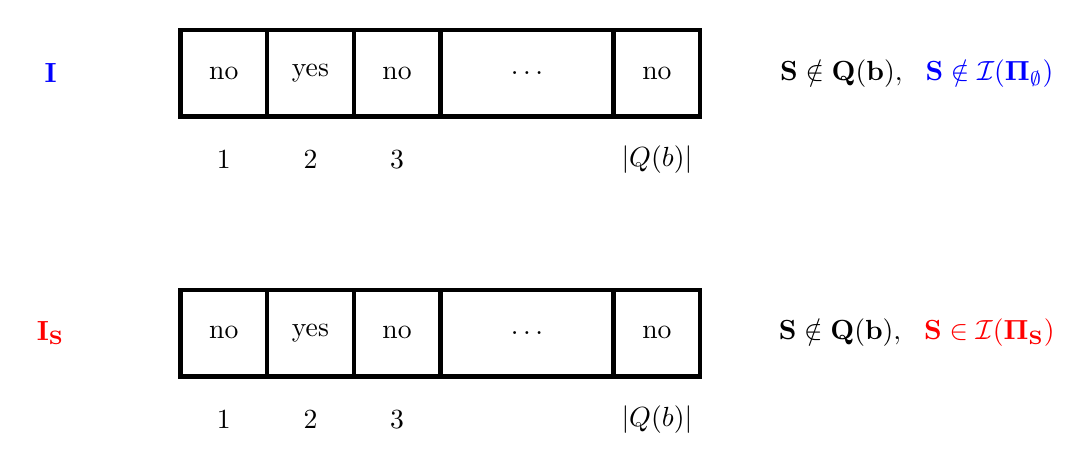
\begin{tikzpicture}[ultra thick,scale=1.1, every node/.style={scale=1}]
		
		
		
		
		\node at (-1.5,3.5) {$\bf \textcolor{blue}{I}$};
		\draw (0,3) rectangle (6,4);
		\draw (1,3)--(1,4);
		\draw (2,3)--(2,4);
		\draw (3,3)--(3,4);
		
		\draw (5,3)--(5,4);
		
		%		\draw (7,0)--(7,1);		
		\draw (6,3)--(6,4);								
		%	\draw (8,3)--(8,4);
		%	\draw (9,3)--(9,4);
		\node at (0.5,2.5) {$1$};
		\node at (0.5,3.5) {no};
		\node at (1.5,2.5) {$2$};
		\node at (1.5,3.5) {yes};
		\node at (2.5,2.5) {$3$};
		\node at (2.5,3.5) {no};
		\node at (4,3.5) {$\ldots$};
		%	\node at (7,3.5) {$\ldots$};
		\node at (5.5,2.5) {$|Q(b)|$};
		\node at (5.5,3.5) {no};
		
		\node at (8.5,3.5) {$\bf \textcolor{black}{S \notin Q(b)},~~ \textcolor{blue}{S \notin \cI(\Pi_{\emptyset})}$};
		%	\node at (10,3.5) {$\ldots$};
		
		%	\node at (8.5,1.3) {$\bf \textcolor{black}{S}$};
		%	\fill[gray, opacity=0.2] (6,3) rectangle (11,4);
		
		% First rectangle I
		\node at (-1.5,0.5) {$\bf \textcolor{red}{I_S}$};
		\draw (0,0) rectangle (6,1);
		\draw (1,0)--(1,1);
		\draw (2,0)--(2,1);
		\draw (3,0)--(3,1);
		
		\draw (5,0)--(5,1);
		
		%	\node at (8.5,4.3) {$\bf \textcolor{black}{S}$};
		
		%		\draw (7,0)--(7,1);		
		\draw (6,0)--(6,1);								
		%			\draw (8,0)--(8,1);
		%	\draw (9,0)--(9,1);
		\node at (0.5,-0.5) {$1$};
		\node at (0.5,0.5) {no};
		\node at (1.5,-0.5) {$2$};
		\node at (1.5,0.5) {yes};
		\node at (2.5,-0.5) {$3$};
		\node at (2.5,0.5) {no};
		\node at (4,0.5) {$\ldots$};
		%	\node at (10,0.5) {$\ldots$};
		%	\node at (7,0.5) {$\ldots$};
		\node at (5.5,-0.5) {$|Q(b)|$};
		\node at (5.5,0.5) {no};
		
		\node at (8.5,0.5) {$\bf \textcolor{black}{S \notin Q(b)},~~ \textcolor{red}{ S \in \cI(\Pi_{S})}$};
		
		
		%	\node at (8.5,1.3) {$\bf \textcolor{black}{S}$};
		%	\fill[gray, opacity=0.2] (6,0) rectangle (11,1);
		%	\node at (0.5,-0.5) {$\x$};
		%		\foreach \x in {1,2,3,4,5,6,7,8,9}{
		%			\draw (\x,0)--(\x,1);
		%			\node at (\x-0.5,-0.5) {$\x$};
		%		}
		%		\node at (10.5,-0.5) {$\ldots$};
		%		\node at (11.5,-0.5) {$Q()b$};
		
		% Second rectangle I_S
		%		\node at (-1,-2.5) {$I_S$};
		%		\draw (0,-3) rectangle (10,-2);
		%		\foreach \x in {1,2,3,4,5,6,7,8,9}{
		%			\draw (\x,-3)--(\x,-2);
		%			\node at (\x-0.5,-3.5) {$\x$};
		%			\node at (\x-0.5,-2.5) {no};
		%		}
		%		\node at (10.5,-3.5) {$\ldots$};
		%		\node at (11.5,-3.5) {$x$};
		%		\node at (11.5,-2.5) {yes};
		%		\node at (11.5,-1.5) {$S$};
		
		\end{tikzpicture}
	\end{center}
	\caption{\label{fig:proof} An illustration of the proof of \Cref{thm:emb}. The figure presents the sequences of queries to the membership oracles by the algorithm on the instances $I$ and $I_S$ for a string of bits $b$, such that $S \notin Q(b)$. The label ''yes" (''no") indicates that the queried set is (not) independent in the matroid. 
		The only query that distinguishes between $I$ and $I_S$ is on the set $S$, which is not queried; thus, the algorithm returns the same output for $I$ and $I_S$.}
\end{figure}


\thmemb*
	\begin{proof}
		Assume towards contradiction that there exist a constant $d \in \mathbb{N}$ and a randomized algorithm $\cA$ that decides every oracle-EMB instance $(E,\cI,c,T)$ in time $\left( (T+2) \cdot n \cdot m \right)^{d}$, where $n = |E|+1$ and $m = c(E)+1$.  
		For every $n,k,\alpha \in \mathbb{N}_{>0}$, consider the set of all subsets of $[n]$ with cardinality $k$ and sum $\alpha$: $$\mathcal{F}_{n,k,\alpha} = \big\{S \subseteq [n]~\big|~|S| = k, \textnormal{\textsf{sum}}(S) = \alpha\big\}.$$ 
		To reach a contradiction, we construct an induced oracle-EMB instance on which $\cA$ does not compute the proper output with sufficiently high probability. The parameters of the instance are extracted from the following combinatorial claim. 
			\begin{claim}
			\label{claim:H1}
			There are $\tilde{n} \in \mathbb{N}_{>0}$, $\tilde{k} \in \left[\tilde{n}\right]$, and $\tilde{\alpha} \in \left[\tilde{n}^2\right]$ such that 
$|\mathcal{F}_{\tilde{n},\tilde{k},\tilde{\alpha}}|> 	2 \cdot \left(	12 \cdot \tilde{n}^5 \right)^{d} $. 
%the following holds
%			\begin{equation*}
%				\begin{aligned}
%						\left(	12 \cdot \tilde{n}^5 \right)^{d} < \frac{2^{\tilde{n}}-1}{2 \cdot \left(\tilde{n}+1\right) \cdot \tilde{n}^2},~~~~~~~~~~~~~	{\tilde{n} \choose \tilde{k}} \geq \frac{2^{\tilde{n}}-1}{\tilde{n}+1}, ~~~~~~~~~~~~~ |\mathcal{F}_{\tilde{n},\tilde{k},\tilde{\alpha}}| \geq  \frac{{\tilde{n} \choose \tilde{k}}}{\tilde{n}^2}. 
%				\end{aligned}
%			\end{equation*}
		\end{claim}
		\begin{claimproof}
				Since $d$ is a constant, %it holds that $$\lim_{n \rightarrow \infty}  \frac{\left(\frac{2^{n}-1}{2 \cdot \left(n+1\right) \cdot n^2}\right)}{\left(	8 \cdot n^5 \right)^{d}} = \infty.$$ Thus, 
				there is $\tilde{n} \in \mathbb{N}_{>0}$ such that 
				\begin{equation}
					\label{eq:nTild}
						\left(	12 \cdot \tilde{n}^5 \right)^{d} < \frac{2^{\tilde{n}}-1}{2 \cdot \tilde{n}^3}.
				\end{equation}
				  Fix $\tilde{n} \in \mathbb{N}_{>0}$ satisfying \eqref{eq:nTild}. Recall that $\sum_{k \in \{0,1,\ldots,\tilde{n}\}} {\tilde{n} \choose k} = 2^{\tilde{n}}$ from a basic property of the Pascal triangle; therefore, $\sum_{k \in \{1,\ldots,\tilde{n}\}} {\tilde{n} \choose k} = 2^{\tilde{n}}-1$. Thus, there is  $\tilde{k} \in \{1,\ldots,\tilde{n}\}$, 
				  such that 
				  \begin{equation}
				  	\label{eq:kTild}
				  	{\tilde{n} \choose \tilde{k}} \geq \frac{2^{\tilde{n}}-1}{\tilde{n}}.
				  \end{equation}
				   Fix $\tilde{k} \in \left[\tilde{n}\right]$ satisfying \eqref{eq:kTild}. Observe that for each $S \in 2^{[\tilde{n}]}$ satisfying $|S| = \tilde{k}>0$, it holds that $1 \leq \textnormal{\textsf{sum}}(S) \leq |S| \cdot \max_{i \in [\tilde{n}]} i = \tilde{n}^2$. Thus, there are $\tilde{n}^2$ possibilities for $\alpha \in \left[\tilde{n}^2\right]$ satisfying $\alpha = \textnormal{\textsf{sum}}(S)$, for some $S \in 2^{[\tilde{n}]}$ such that $|S| = \tilde{k}$. Moreover, there are ${\tilde{n} \choose \tilde{k}}$ subsets of $[\tilde{n}]$ of cardinality $\tilde{k}$. By the pigeonhole principle, there is $\tilde{\alpha} \in  \left[  \tilde{n}^2 \right]$ such that $|\mathcal{F}_{\tilde{n},\tilde{k},\tilde{\alpha}}| \geq  \frac{{\tilde{n} \choose \tilde{k}}}{\tilde{n}^2}$. Thus,
				   $$|\mathcal{F}_{\tilde{n},\tilde{k},\tilde{\alpha}}| \geq \frac{{\tilde{n} \choose \tilde{k}}}{\tilde{n}^2}  \geq  \frac{2^{\tilde{n}}-1}{\tilde{n} \cdot \tilde{n}^2} > 2 \cdot \left(	12 \cdot \tilde{n}^5 \right)^{d}.$$ The second inequality follows from \eqref{eq:kTild}, and the third inequality holds by \eqref{eq:nTild}. 
		\end{claimproof}
		
	

		
		Let $\tilde{n} \in \mathbb{N}_{>0}$, $\tilde{k} \in \left[\tilde{n}\right]$, and $\tilde{\alpha} \in \left[\tilde{n}^2\right]$  satisfying the conditions of \Cref{claim:H1}. Define $t$ to be the maximum running time of $\cA$ on an induced EMB instance $I_{\tilde{n},\tilde{k},\tilde{\alpha}}(\Pi)$ over all $\Pi \in 2^{\left[ \tilde{n}\right]}$. 
			\begin{claim}
			\label{claim:H2}
			$t \leq	\left(	12 \cdot \tilde{n}^5 \right)^{d}$.    
		\end{claim}
		\begin{claimproof}
				Let $T = \tilde{\alpha}$, $n = \tilde{n}+1$, and $m = \textsf{id}_{\tilde{n}}(\left[\tilde{n}\right])+1$. By the running time guarantee of $\cA$, it follows that $t \leq	\left(	n \cdot (T+2) \cdot m \right)^{d}$. It remains to bound $n \cdot (T+2) \cdot m$. Since $\textsf{id}_{\tilde{n}}(\left[\tilde{n}\right]) = \textsf{sum}(\left[\tilde{n}\right])$ and $\tilde{\alpha} \leq \tilde{n}^2$, %By the definition of induced EMB instance (\Cref{def:EMBpi}) with parameters $\tilde{n},\tilde{k},\tilde{\alpha}$,
				 \begin{equation*}
				\label{eq:InducedParameters}
				%(\tilde{\alpha} +1) \cdot \left( \textsf{id}_{\tilde{n}} ( \left[\tilde{n} \right])+1 \right) \cdot \left(\tilde{n}+1\right) 
				n  \cdot (T+2) \cdot m \leq	 \left(\tilde{n}+1\right) \cdot \left( \tilde{n}^2+2\right)\left( \textsf{sum}( \left[\tilde{n} \right])+1 \right) \leq 2 \tilde{n} \cdot 3 \tilde{n}^2 \cdot \left(\frac{\tilde{n} \cdot (\tilde{n}+1)}{2}+1 \right) \leq 12 \cdot \tilde{n}^5. 
			\end{equation*}  The second inequality follows from the sum of the terms of an arithmetic sequence. By the above and the running time guarantee of $\cA$, it follows that $t \leq	\left(	n \cdot (T+2) \cdot m \right)^{d} \leq 	\left(	12 \cdot \tilde{n}^5 \right)^{d}$.   
		\end{claimproof}
		
	Given  an induced oracle-EMB instance $I_{\tilde{n},\tilde{k},\tilde{\alpha}}(\Pi)$, for some $\Pi \subseteq \left[ \tilde{n}\right]$,  the randomized algorithm $\cA$ produces a random string of bits $\bar{b} \in \{0,1\}^{t}$ and performs a sequence of queries to the membership oracle of $M_{\tilde{n},\tilde{k},\tilde{\alpha}}$, based on $\bar{b},\tilde{n},\tilde{k},\tilde{\alpha}$, and the results of the previous queries; then, the algorithm decides the given instance based on the queries. 
		 
		 
		 Let $\Pi_{\emptyset} = \emptyset$, and consider the induced oracle-EMB instance $I = I_{\tilde{n},\tilde{k},\tilde{\alpha}}(\Pi_{\emptyset})$. Given a string of bits $b \in \{0,1\}^{t}$, let $Q(b) \subseteq 2^{[\tilde{n}]}$ be the set of  all subsets $S \subseteq [\tilde{n}]$ queried by $\cA$ on the instance $I$ and the bit-string $b$ (on the membership oracle of $M_{\tilde{n},\tilde{k},\tilde{\alpha}}(\Pi_{\emptyset})$). For clarity, we use $\bar{b}$ for a random string, and $b$ for a realization of $\bar{b}$ to a specific string. Note that $Q(b)$ is a set, since the algorithm is deterministic for every $b \in \{0,1\}^{t}$; conversely, $Q(\bar{b})$ is a random set for a random string $\bar{b} \in \{0,1\}^{t}$. As the running time of $\cA$ on %an induced EMB instance with $\tilde{n}$ elements and rank parameter $\tilde{k}$ 
		$I$ is bounded by $t$, it holds that $|Q(b)| \leq t$ for every $b \in \{0,1\}^{t}$. Let 
		\begin{equation*}
			\label{eq:R}
			R(I) = \left\{S \in \mathcal{F}_{\tilde{n},\tilde{k},\tilde{\alpha}}~\bigg|~\Pr \left(S \in Q(\bar{b}) \right) \geq \frac{1}{2} \right\}
		\end{equation*} be all sets in $ \mathcal{F}_{\tilde{n},\tilde{k},\tilde{\alpha}}$ that are queried by $\cA$ with probability  at least $\frac{1}{2}$. 
			\begin{claim}
			\label{claim:H3}
			$|R(I)|  < |\mathcal{F}_{\tilde{n},\tilde{k},\tilde{\alpha}}|$. 
		\end{claim}
		\begin{claimproof}
			By the definition of $R(I)$, it holds that 
				\begin{equation*}
				\label{eq:R0}
				\begin{aligned}
					|R(I)| ={} & \left| \left\{S \in \mathcal{F}_{\tilde{n},\tilde{k},\tilde{\alpha}}~\bigg|~\Pr \left(S \in Q(\bar{b}) \right) \geq \frac{1}{2} \right\} \right| \\
					\leq{} & 2 \cdot \sum_{S \in \mathcal{F}_{\tilde{n},\tilde{k},\tilde{\alpha}}} \Pr \left(S \in Q(\bar{b}) \right)  \\
					={} & 	 2 \cdot \sum_{S \in \mathcal{F}_{\tilde{n},\tilde{k},\tilde{\alpha}}~} \sum_{b \in \{0,1\}^{t}} \Pr \left(S \in Q(b) \right) \cdot \Pr(\bar{b} = b)
				\end{aligned}
			\end{equation*} Thus, by changing the order of summation, we have 
				\begin{equation*}
				\begin{aligned}
					|R(I)| \leq 2 \cdot  \sum_{b \in \{0,1\}^{t}~} \Pr(\bar{b} = b) \cdot \sum_{S \in \mathcal{F}_{\tilde{n},\tilde{k},\tilde{\alpha}}} \Pr \left(S \in Q(b) \right) 
					\leq 2 \cdot  \sum_{b \in \{0,1\}^{t}~} \Pr(\bar{b} = b) \cdot |Q(b)| .
				%	\leq {} &  2  t \cdot \sum_{b \in \{0,1\}^{t}~} \Pr (\bar{b} = b).
				\end{aligned}
			\end{equation*} 
			
Since $\left|Q(b)\right| \leq t$ for all $b \in \{0,1\}^t$, by the above we have
			\begin{equation*}
				|R(I)| 	\leq 2  t \cdot \sum_{b \in \{0,1\}^{t}~} \Pr (\bar{b} = b) = 2  \cdot t \leq 2\cdot	\left(	12 \cdot \tilde{n}^5 \right)^{d} 
		%		<   \frac{2^{\tilde{n}}-1}{\left(\tilde{n}+1\right) \cdot \tilde{n}^2} \leq  \frac{{\tilde{n} \choose \tilde{k}}}{\tilde{n}^2} 
				< |\mathcal{F}_{\tilde{n},\tilde{k},\tilde{\alpha}}|. 
			\end{equation*}
			The second inequality follows from \Cref{claim:H2}. The last inequality holds by \Cref{claim:H1}. 
		\end{claimproof}
	
	By \Cref{claim:H3}, there exists $S \in F_{\tilde{n},\tilde{k},\tilde{\alpha}} \setminus R(I)$. %; thus, $\Pr \left( S \in Q(\bar{b}) \right) < \frac{1}{2}$. Now, 
		Consider the induced oracle-EMB instance %$I_S = (\tilde{n},\tilde{k},\alpha,M_{\tilde{n},\tilde{k},\alpha}(\Pi_{S}))$ 
		$I_S = I_{\tilde{n},\tilde{k},\tilde{\alpha}}(\Pi_S)$ where $\Pi_{S} = \{S\}$, and let $B = \{b \in \{0,1\}^t~|~ S \notin Q(b)\}$ be all strings for which $S$ is not queried by $\cA$ on the instance $I$ .
	Observe that for all $b \in B$ it holds that the answers to all queries for $T \in Q(b)$ are the same for both oracles (of $M_{\tilde{n},\tilde{k},\tilde{\alpha}}(\Pi_{\emptyset})$ and $M_{\tilde{n},\tilde{k},\tilde{\alpha}}(\Pi_{S})$). Moreover, the decision on which set to query next depends only on $b,\tilde{n},\tilde{k},\tilde{\alpha}$, and the answers to previous queries.  
	
	Hence, for all $b \in B$,  the executions of $\cA$ on the instances $I$ and $I_S$ are identical.
		Since $\Pi_{\emptyset} = \emptyset$, by %\eqref{eq:1} and \Cref{def:EMBpi} 
		\Cref{obs:YesNo}, $I$ is a ``no''-instance for oracle-EMB; thus, $\cA$ returns that $I_S$ is a ``no''-instance for every $b\in B$. However, since $\textsf{id}_n(S) = \textsf{sum}(S) = \alpha$, $|S| = k$, and $S \in \Pi_{S}$, it follows that $I_S$ is a ``yes''-instance by \Cref{obs:YesNo}.  
%		does not query the membership oracle of $M_{\tilde{n},\tilde{k},\alpha}(\Pi_{S})$ with $S$; %The reason is that the answers to all queries in $Q(b)$ are the same for both oracles (of $M_{n,k,\alpha}(\Pi_{\emptyset})$ and $M_{n,k,\alpha}(\Pi_{S})$), and the decision which sets to query next depends only on $b,n,k,\alpha$, and the answers to previous queries.  
		%
		% $Pr[\bar{b} = b] = Pr[b(I_S) = b]$ since the inputs $I$ and $I_S$ are completely similar besides the membership oracle. Thus, $Pr[S \in Q(b(I_S))] = Pr[S \in Q(\bar{b})] < \frac{1}{2}$. 
		%
		Therefore, $\cA$ does not decide $I_S$ correctly for all $b \in B$.  We give an illustration in \Cref{fig:proof}. Since  $S \notin R(I)$, it holds that $\Pr \left( \bar{b} \in B \right) = \Pr \left(S \notin Q(\bar{b}) \right) > \frac{1}{2}$; thus, with probability greater than $\frac{1}{2}$, $\cA$ does not decide correctly the instance $I_S$. 
		%
		%Therefore, w.p. strictly larger than $\frac{1}{2}$ algorithm $\cA$ does not query $S$ for the instance $I_S$. Hence, w.p. strictly larger than $\frac{1}{2}$ algorithm $\cA$ performs the exact same computations on $I$ and $I_S$ and must return the same result. %Note that if the algorithm does not query $S$ it cannot decide correctly the instance $I_S$, since $S$ is the unique solution of $I_S$. 
		%Since $\mathcal{L}_{n,k,\alpha}(\Pi_{\emptyset}) = \emptyset$ and $\mathcal{L}_{n,k,\alpha}(\Pi_{S}) \neq \emptyset$, we conclude that algorithm $\cA$ cannot decide correctly w.p. at least $\frac{1}{2}$ both $I$ and $I_S$, which 
		A contradiction to the correctness of  $\cA$  as a randomized algorithm for oracle-EMB. The statement of the theorem follows. 
	\end{proof}
	
	
	
	

	
\section{Hardness of Matroid Optimization with a Linear Constraint}
\label{sec:tight_absolute}
In this section we use \Cref{thm:emb} %and \Cref{cor:deter} 
to prove \Cref{thm:main}. We apply the following reductions from EMB to MOL problems. Recall that $\cQ = \cP \setminus \{(\min,\IS,\leq)\}$ is the set of parameters for non-trivial MOL problems. Given a $P$-MOL problem for some $P \in \cQ$, and an EMB instance $I$, the reduction returns an instance $R_P(I)$ of the $P$-MOL problem. Note that the reduction is purely mathematical, and 
% in the sense that it 
does not specify the encoding of the instance. This will be useful for obtaining our hardness results in non-oracle computational models (see \Cref{sec:SAT}). 

Given $(\opt,\cF,\triangleleft), (\opt',\cF',\triangleleft') \in \cQ$, we use the notation $(\opt \textnormal{ is } \opt')$,  $(\cF \textnormal{ is } \cF')$, $(\triangleleft \textnormal{ is } \triangleleft')$ to denote the boolean expressions of equality between parameters of a MOL problem. For example, $(\opt \textnormal{ is } \opt')$ is {\em true} if and only if either $\opt,\opt'$ are both $\max$, or $\opt,\opt'$ are both $\min$. 

%$(\opt \textnormal{ is } \max)$ and $(\opt' \textnormal{ is } \max)$ are true, or $(\opt \textnormal{ is } \min)$ and $(\opt' \textnormal{ is } \min)$ are true. 


\begin{definition}
	\label{def:reduction}
	Given an \textnormal{EMB} instance $I =(E,\cI,c,T)$ and  $P \in \cQ$ where $P = (\opt,\cF,\triangleleft)$, define the
	 {\em reduced $P$-MOL instance} of $I$, denoted by  $R_P(I) = (E,\cI,v_I,w_{I,P},L_{I,P})$, as follows.
	\begin{enumerate}
		\item Define the auxiliary variable 
		\begin{align*}
			%	n & : \text{The variable representing a natural number.} \\
			d(P) = & \begin{cases}
				0 & ~~\textnormal{if  } \bigg((\opt \textnormal{ is } \max)  \textnormal{ and }   (\triangleleft \textnormal{ is}   \leq) \bigg) \textnormal{ or } 
				\bigg((\opt \textnormal{ is } \min)  \textnormal{ and }   (\triangleleft \textnormal{ is}   \geq) \bigg)\\
				1 & ~~\textnormal{otherwise.}
			\end{cases}
		\end{align*} For example, if $P = (\max,\IS,\leq)$ then $d(P) = 0$, and if  $P' = (\max,\IS,\geq)$ then $d(P') = 1$. 
		\item Let $H_I = 2 \cdot \max \{1, c(E)\}$.
		\item For all $e \in E$ let $v_I(e) =  H_I +c(e)$. 
		\item For all $e \in E$ let $w_{I,P}(e) =  H_I +c(e) \cdot (-1)^{d(P)}$.
		\item Let $k_I = \max_{S \in \cI} |S|$ be the rank of $(E,\cI)$. 
		\item Define $L_{I,P} = k_I \cdot H_I +T \cdot  (-1)^{d(P)}$. 
	\end{enumerate}
\end{definition}


%learly, given an EMB instance $I$ and $P \in \cQ$ the $P$-MOL instance $R_P(I)$ can be computed in polynomial time. 
%The main properties of the reduction are summarized in the following theorem. 
Now, for every EMB instance $I =(E,\cI,c,T)$, define the {\em error parameter} of $I$ as \begin{equation}
\label{eq:epsI}
\eps_I =  \frac{1}{8 \cdot (|E|+1) \cdot (T+1) \cdot \left(c(E)+1\right)}.
\end{equation}
Indeed, since the value selected for of the error parameter is sufficiently small, we can use a $(1+\eps_I)$-approximation for $R_P(I)$ to decide an EMB instance $I$.  
\begin{restatable}{theorem}{thmH}
	\label{thm:H}
	Given an instance $I =(E,\cI,c,T)$ of \textnormal{EMB}, and $P \in \cQ$ with $P = (\opt,\cF,\triangleleft)$, the following holds. 
	\begin{enumerate}
		\item If there is a solution $S$ for $R_P(I)$ such that $v_I(S) = k_I \cdot H_I +T$, then $I$ is a ``yes"-instance.  \label{h:1}
		\item  If $I$ is a ``yes"-instance then: %$I$ has a solution then: 
		$(i)$ $R_P(I)$ has a solution, and $(ii)$ every $(1+\eps_I)$-approximate solution $S$ for $R_P(I)$ satisfies $v_I(S) = k_I \cdot H_I +T$. \label{h:2}
	\end{enumerate}
\end{restatable}
Using \Cref{thm:H} and an assumed randomized Fully PTAS for the $P$-MOL problem, we can decide EMB in time which contradicts \Cref{thm:emb}. This gives the proof of \Cref{thm:main}. We first prove \Cref{thm:main}, and later give the proof of \Cref{thm:H}.   

 \thmMain*

\begin{proof}
	Assume towards a contradiction that there is a randomized Fully PTAS $\cA$ for oracle $P$-MOL. We use $\cA$ to decide oracle-EMB. Let $I = (E,\cI,c,T)$  be an oracle-EMB instance, and %let $n = |E|+1$ and let $m = c(E)+1$; observe that $n,m \neq 0$. C
	consider the following randomized algorithm $\cB$ that decides $I$. 
	\begin{enumerate}
		\item Construct the oracle $P$-MOL instance $R_{P}(I)$
		with the membership oracle of $(E,\cI)$.\label{step:1} 
		\item 
		Execute $\cA$ with the input $R_{P}(I)$ and $\eps_I$. \label{step:2} 
		\item If $\cA$ returns that $R_{P}(I)$ does not have a solution $-$ Return ''no" on $I$. \label{step:3}  %does not have a solution. \label{step:3} 
		\item Otherwise, let $S \leftarrow \cA(R_{P}(I),\eps_I)$ be the solution returned  by $\cA$.\label{step:4} 
		\item Return ''yes" on $I$ if and only if $v_I(S) = H_I \cdot k_I+T$. \label{step:5} 
	\end{enumerate}
	
	Let $n = |E|+1$ and $m = c(E)+1$. Note that $R_{P}(I)$ can be naively constructed from $I$ in time $\left(n \cdot (T+2) \cdot m\right)^{O(1)}$ using \Cref{def:reduction}. 
	As $\cA$ is a randomized Fully PTAS for oracle $P$-MOL, and by the selection of the error parameter \eqref{eq:epsI}, the running time of $\cB$ on $I$ is $\left(n \cdot (T+2) \cdot m\right)^{O(1)}$. %For the correctness,
	We now show correctness. 
	\begin{itemize}
		\item If $\cB$ returns ``yes" on $I$, then Step~\ref{step:4} of the algorithm computes a solution $S$ for $R_p(I)$ satisfying $v_I(S) = H_I \cdot k_I+T$. Thus, by \Cref{thm:H}, $I$ is a ``yes" instance. %has a solution.   
		
		
		\item If $I$ is a ``yes" instance then $R_P(I)$ has a solution by \Cref{thm:H}.
		As $\cA$ is a randomized Fully PTAS, with probability at least $\frac{1}{2}$ $\cA$ returns a $(1+\eps_I)$-approximate solution $S$ for $R_P(I)$ in Step~\ref{step:4}. By \Cref{thm:H}, $v_I(S) = H_I \cdot k_I+T$ (with probability at least $\frac{1}{2}$). Thus, $\cB$ returns ``yes" on $I$ with probability at least $\frac{1}{2}$.
		\end{itemize}  Hence, $\cB$ is a randomized algorithm which decides the oracle-EMB instance $I$ in time \newline $\left(n \cdot (T+2) \cdot m\right)^{O(1)}$. This is a contradiction to \Cref{thm:emb}.  
\end{proof}













In the remainder of this section we prove \Cref{thm:H}. We start with some basic properties of the reduction outlined in \Cref{def:reduction}.   

\begin{lemma}
\label{lem:FD2}
Given an instance $I =(E,\cI,c,T)$ of \textnormal{EMB},
let $P \in \cQ$ and consider a solution $S$ for $R_P(I)$ satisfying $v_I(S) = k_I \cdot H_I+T$. Then, $S$ is a solution for $I$.  
\end{lemma}

\begin{proof}
	Let $\cm = (E,\cI)$. As $S$ is a solution for $R_P(I)$, it holds that $S \in \IS(\cm)$; thus, $|S| \leq k_I$. Assume towards contradiction that $|S|<k_I$. Then, 
	$$v_I(S) = |S| \cdot H_I+c(S) \leq (k_I-1) \cdot H_I+c(S) \leq (k_I-1) \cdot H_I+c(E)<k_I \cdot H_I \leq k_I \cdot H_I+T.$$ 
	We reach a contradiction since $v_I(S) = k_I \cdot H_I+T$; thus, $|S| = k_I$, and  
	\begin{equation}
		\label{eq:S=k}
		k_I \cdot H_I+T = v_I(S) =   |S| \cdot H_I+c(S) =  k_I \cdot H_I+c(S). 
	\end{equation}  As $|S| = k_I$, we have that $S$ is a basis of $\cm$, and by \eqref{eq:S=k}, $c(S) = T$. Hence, $S$ is a solution for $I$.   
\end{proof}

The next result is the converse of the statement in \Cref{lem:FD2}.   

	\begin{lemma}
	\label{lem:FD1}
	Let $S$ be a solution for a given \textnormal{EMB} instance $I =(E,\cI,c,T)$,
	and let $P \in \cQ$ where $P = (\opt,\cF,\triangleleft)$. Then, $S$ is a solution for $R_P(I)$ of value $v_I(S) = k_I \cdot H_I+T$.  %be a non-trivial  \textnormal{MOL} problem, where $P = (\opt,\cF,\triangleleft)$. 
\end{lemma}

\begin{proof}
	Let $\cm = (E,\cI)$. Since $S$ is a solution for $I$ we have $S \in \bases(\cm)$; thus, $S \in \cF(\cm)$. Then,    
	$$w_{I,P}(S) = |S| \cdot H_I+c(S) \cdot (-1)^{d(P)} =  k_I \cdot H_I+T \cdot (-1)^{d(P)} = L_{I,P}.$$
	The second equality holds since $S$ is a solution for $I$; thus, $|S| = k_I$ (as $S$ is a basis of $\cm$), and $c(S) = T$. We conclude that $S$ is a solution for $R_P(I)$. Finally, note that $S$ satisfies 
%	\begin{equation*}
%		\label{eq:t=r}
%		v_I(S) = |S| \cdot H_I+c(S) =  k_I \cdot H_I+T.
%		\end{equation*}\end{proof}
\begin{align*}
~~~~~~~~~~~~~~~~~~~~~~~~~~~~~	v_I(S) = |S| \cdot H_I + c(S)
	= k_I \cdot H_I +T ~~~~~~~~~~~~~~~~~~~~~~~~~~~~~~~~~~~~~~~~~~~~~~~~~~~~~~~~ \qedhere
\end{align*}
\end{proof}

The next claim gives an upper bound on the optimal value for maximization MOL problems. We then derive an analogous lower bound for minimization (non-trivial) MOL problems. 











	\begin{lemma}
	\label{lem:OptMaxBound}
	Let $I =(E,\cI,c,T)$ be an \textnormal{EMB} instance and $P \in \cQ$, where $P = (\opt,\cF,\triangleleft)$ and $\left(\opt \textnormal{ is } \max\right)$. Then, for every solution $S$ of $R_P(I)$ it holds that $v_I(S) \leq k_I \cdot H_I+T$.  %be a non-trivial  \textnormal{MOL} problem, where $P = (\opt,\cF,\triangleleft)$. 
\end{lemma}

\begin{proof}
	Let $S$ be an optimal solution for $R_P(I)$. Thus, $|S| \leq k_I$ as $S \in \cI$. If $|S| < k_I$ then
	%\begin{itemize}
	%	\item If $d(P) = 0$. Then, consider the following sub cases.  
	 \begin{equation*}
			v_I(S) \leq (k_I-1) \cdot H_I+c(S) \leq (k_I-1) \cdot H_I+c(E) <k_I \cdot H_I \leq k_I \cdot H_I+T.
		\end{equation*}
	%	and 
%		\begin{equation}
%			\label{eq:S<Kv}
%			w_{I,P}(S) \leq (k-1) \cdot H_I+c(S)\cdot (-1)^{d(P)} \leq (k-1) \cdot H_I+c(E) <2k \cdot c(E) \leq k_I \cdot H_I+T.
%		\end{equation}
	Otherwise, $|S| = k_I$. Consider the two cases for $\triangleleft$.
			\begin{enumerate}
		\item $(\triangleleft \textnormal{ is}   \leq)$. Then, $d(P) = 0$ (see \Cref{def:reduction}); thus, since $S$ is a solution for $R_P(I)$: $$v_I(S) = w_{I,P}(S) \leq L_{I,P} = k_I \cdot H_I+T.$$ 
		\item $(\triangleleft \textnormal{ is}   \geq)$. Then, $d(P) = 1$. As $S$ is a solution for $R_P(I)$,
		\begin{equation}
			\label{eq:Dp=1}
			  k_I \cdot H_I-c(S)=|S|\cdot H_I-c(S) =w_{I,P}(S) \geq L_{I,P} = k_I \cdot H_I-T.
		\end{equation} 
		By \eqref{eq:Dp=1}, it follows that $c(S) \leq T$; thus, $	v_I(S) = k_I \cdot H_I+c(S) \leq k_I \cdot H_I+T$. 
	\end{enumerate} 
	% E.g., for $P = (\max,\IS,\leq)$ it holds that $d(P) = 0$ and for  $P' = (\max,\IS,\geq)$ it is $d(P') = 1$. 
	
%		\begin{enumerate}
%			\item $d(P) = 0$. Then, it follows that $\triangleleft = \leq $; thus, since $S$ is a solution for $R_P(I)$: $$v_I(S) = w_{I,P}(S) \leq L_{I,P} = k_I \cdot H_I+T.$$ 
%			\item $d(P) = 1$. Then, $\triangleleft = \geq $; thus, since $S$ is a solution for $R_P(I)$:
%			\begin{equation}
%				\label{eq:Dp=1}
%				w_{I,P}(S) = k \cdot H_I-c(S) \geq L_{I,P} = k \cdot H_I-T.
%			\end{equation} 
%			By \eqref{eq:Dp=1} it follows that $c(S) \leq T$; thus, $	v_I(S) = k \cdot H_I+c(S) \leq k_I \cdot H_I+T$. 
%		\end{enumerate} 
In all the above cases, we have that $v_I(S) \leq k_I \cdot H_I+T$, implying the statement of the lemma. 
\end{proof}

Now, for minimization problems we have the next result. 
	\begin{lemma}
	\label{lem:OptMinBound}
	Let $I =(E,\cI,c,T)$ be an \textnormal{EMB} instance, and $P \in \cQ$, where $P = (\opt,\cF,\triangleleft)$ and $\left(\opt \textnormal{ is } \min\right)$. Then, for every solution $S$ of $R_P(I)$, it holds that $v_I(S) \geq k_I \cdot H_I+T$.  %$\OPT\left( R_P(I) \right) \geq k_I \cdot H_I+T$.  %be a non-trivial  \textnormal{MOL} problem, where $P = (\opt,\cF,\triangleleft)$. 
\end{lemma}

\begin{proof}
	Let $S$ be a solution for $R_P(I)$. We consider two cases. 
	\begin{enumerate}
		\item $(\triangleleft \textnormal{ is}   \geq)$. Then, $d(P) = 0$; since $S$ is a solution for $R_P(I)$, $$v_I(S) = w_{I,P}(S) \geq L_{I,P} = k_I \cdot H_I+T.$$ 
		\item  $(\triangleleft \textnormal{ is}   \leq)$. Then, $d(P) = 1$; since $P$ is a non-trivial MOL problem (i.e., $P \in \cQ$), it follows that $\left(\cF \textnormal{ is } \bases\right)$. Thus, $S$ is a solution for $R_P(I)$ such that $|S| = k_I$, and
		\begin{equation}
			\label{eq:Dp=2}
			 	  k_I \cdot H_I-c(S)= |S| \cdot H_I-c(S) =w_{I,P}(S) \leq L_{I,P} = k_I \cdot H_I-T.
		\end{equation} 
		By \eqref{eq:Dp=2} it follows that $c(S) \geq T$; thus, $v_I(S) = k_I \cdot H_I+c(S) \geq k_I \cdot H_I+T$. 
	\end{enumerate}
	%	\end{itemize} 
%\item 
%\end{itemize}
In all of the above cases, we have that $v_I(S) \geq k_I \cdot H_I+T$, implying the statement of the lemma. 
\end{proof}


Using \Cref{lem:FD1,lem:FD2,lem:OptMaxBound,lem:OptMinBound}, we can now prove \Cref{thm:H}. 
\thmH*
\begin{proof}
%	The first property the theorem
We note that Property~\ref{h:1} follows directly from \Cref{lem:FD2}. For Property~\ref{h:2}, assume that $I$ is a ``yes"-instance, then by \Cref{lem:FD1}, there is a solution $D$ for $R_P(I)$ such that $v_I(D) = H_I \cdot k_I+T$. It remains to show Property~\ref{h:2}. $(ii)$.
%that every $(1+\eps_I)$-approximate solution $S$ for $R_P(I)$ satisfies $v_I(S) = H_I \cdot k_I+T$.
Let $S$ be a $(1+\eps_I)$-approximate solution for $R_P(I)$. We distinguish between two cases. 
	
		\begin{enumerate}
		\item $(\opt \textnormal{ is}   \max)$. Then, by \Cref{lem:OptMaxBound},
		\begin{equation*}
			\label{eq:Max1}
			0 \leq H_I \cdot k_I+T-v_I(S).
		\end{equation*} Moreover, since $S$ is a $(1+\eps_I)$-approximate solution for $R_P(I)$, and $D$ is a solution for $R_P(I)$,
		\begin{equation*}
			\label{eq:MaxApprox}
	%	0 \leq 
	H_I \cdot k_I+T-v_I(S) \leq H_I \cdot k_I+T - \frac{v_I(D)}{(1+\eps_I)} =  \frac{\eps_I \cdot \left(H_I \cdot k_I+T \right) }{(1+\eps_I)} \leq \eps_I \cdot \left(H_I \cdot k_I+T \right). 
		\end{equation*} %The first inequality follows from \Cref{lem:OptMaxBound}. 
	%	The second inequality holds since $S$ is a $(1+\eps_I)$-approximation for $R_P(I)$ and $D$ is some solution for $R_P(I)$. 
	By the above, it follows that%\eqref{eq:Max1} and \eqref{eq:MaxApprox} it follows that 
	\begin{equation*}
			  \left|	v_I(S)-\left(H_I \cdot k_I+T\right) \right|	\leq 	\eps_I \cdot \left(H_I \cdot k_I+T\right). 
	\end{equation*}
		\item  $(\opt \textnormal{ is}   \min)$. This case is analogous to the above.  By \Cref{lem:OptMinBound}, 
		\begin{equation*}
			\label{eq:Min1}
	0 \leq v_I(S) - \left(H_I \cdot k_I+T\right). 
		\end{equation*} Since $S$ is a $(1+\eps_I)$-approximate solution for $R_P(I)$, and $D$ is a solution for $R_P(I)$,
		\begin{equation*}
			\label{eq:MinApprox}
			%	0 \leq 
		v_I(S) - \left(H_I \cdot k_I+T\right) \leq (1+\eps_I) \cdot v_I(D) - \left(H_I \cdot k_I+T\right) =   \eps_I \cdot \left(H_I \cdot k_I+T \right). 
		\end{equation*} 
		By the above, 
		\begin{equation*}
			\left|	v_I(S)-\left(H_I \cdot k_I+T\right) \right|	\leq 	\eps_I \cdot \left(H_I \cdot k_I+T\right). 
		\end{equation*}

	\end{enumerate} 
	Thus in both cases it holds that, 
	\begin{equation}
		\label{eq:combined}
		\left|	v_I(S)-\left(H_I \cdot k_I+T\right) \right|	\leq 	\eps_I \cdot \left(H_I \cdot k_I+T\right). 
	\end{equation}
	Let $n = |E|+1$ and $m = c(E)+1$. Then, by the selection of $\eps_I$ in \eqref{eq:epsI}, 
	\begin{equation}
		\label{eq:MinMax}
		\eps_I \cdot \left(H_I \cdot k_I+T\right) = \frac{H_I \cdot k_I+T}{8 \cdot n \cdot (T+1) \cdot m} 
		\leq\frac{2 \cdot m \cdot n + T}{8 \cdot n \cdot (T+1) \cdot m} 
		<\frac{4 \cdot m \cdot n \cdot (T+1)}{8 \cdot n \cdot (T+1) \cdot m} 
		= \frac{1}{2}. 
	\end{equation}
The first inequality holds since $k_I \leq |E|$ and $H_I \leq 2 \cdot m$.	Therefore, by \eqref{eq:combined} and \eqref{eq:MinMax}, 
	\begin{equation}
		\label{eq:FinalMinMax}
		  \left|	v_I(S)-\left(H_I \cdot k_I+T\right) \right|	\leq 	\eps_I \cdot \left(H_I \cdot k_I+T\right) <  \frac{1}{2}.
	\end{equation} Since $v_I(S) \in \mathbb{N}$ by \Cref{def:reduction}, it follows from \eqref{eq:FinalMinMax} that $v_I(S) = H_I \cdot k_I+T$. This gives
	the statement of the theorem. 
\end{proof}

   		    
	%	\section{Tight Lower Bounds using $\Pi$-Matroids}
\label{sec:tight_absolute}
In this section we use \Cref{thm:emb} and \Cref{cor:deter} to prove \Cref{thm:main}. We rely on the following reduction.

\begin{definition}
	Given an \textnormal{EMB} instance $I =(E,\cI,c,k,T)$ and non-trivial  \textnormal{MOL} problem $P \in \cP \setminus \{(\min,\IS,\leq)\}$ where $P = (\opt,\cF,\triangleleft)$, define $R_P(I) = (E,\cI,v_I,w_{I,P},B_{I,P})$ as the {\em reduced} $P$ instance of $I$ as follows.
	\begin{enumerate}
		\item Define the following auxiliary variable \begin{align*}
		%	n & : \text{The variable representing a natural number.} \\
			d(P) = & \begin{cases}
				0 & ~~\text{if  } \left(\opt = \max, \triangleleft = \leq \right) \text{ or } \left(\opt = \min, \triangleleft = \geq \right) \\
			1 & ~~\text{otherwise.}
			\end{cases}
		\end{align*}
		
		\item For all $e \in E$ define $v_I(e) = 2 \cdot c(E)+c(e)$. 
		\item For all $e \in E$ define $w_{I,P}(e) = 2 \cdot c(E)+c(e) \cdot (-1)^{d(P)}$.
		\item Define $B_{I,P} = k \cdot 2 \cdot c(E)+T \cdot  (-1)^{d(P)}$. 
	\end{enumerate}
\end{definition}



%, our lower bounds for {\sc budgeted matroid independent set}, {\sc exact weight matroid independent set}, {\sc constrained minimum weight basis of a matroid}, and {\sc knapsack cover with a matroid}. All proofs use reductions from the $\Pi$-matroid problem.

%In all of the constructions, we are able to use (with slight modifications) the same family of {\em standard weight} functions and {\em standard budgets}. 


%Specifically, for every $n \in \mathbb{N}_{>0}$ define the standard weight function of $n$ as $w_{n}:[n] \rightarrow \mathbb{N}$ such that for all $i \in [n]$
% \begin{equation}
%	\label{eq:w}
%	w_{n}(i) = i+2 \cdot \textnormal{\textsf{sum}}([n]). 
%\end{equation}
%Also, define the standard budget of  $n,k,\alpha \in \mathbb{N}_{>0}$  as 
%\begin{equation}
%	\label{eq:B}
%	B_{n,k,\alpha} = \alpha+2 k \cdot \textnormal{\textsf{sum}}([n]). 
%\end{equation}

%In deriving the lower bounds for our problems (in
%\Cref{sec:abs_BM,sec:abs_EMI,sec:abs_CMB,sec:abs_KCM}), we use some general results, as stated in \Cref{lem:OPTu,lemma:if,lemma:onlyif}.
The following lemma gives a polynomial bound on the total weight of any subset of the ground set of a reduced instance. 

\begin{lemma}
	\label{lem:OPTu}
%	For every $n \in \mathbb{N}_{>0}$ and $S \subseteq [n]$, it holds that $w_{n}(S) \in \{0,1,\ldots, 3 \cdot n^3\}$. 
	Given an \textnormal{EMB} instance $I =(E,\cI,c,k,T)$ and non-trivial  \textnormal{MOL} problem $P \in \cP \setminus \{(\min,\IS,\leq)\}$ where $P = (\opt,\cF,\triangleleft)$, for every $S \subseteq E$ it holds that $v_{I}(S) \in \{0,1,\ldots, 2 \cdot c(E) \cdot k\}$.  
\end{lemma}

\begin{proof}
	By \eqref{eq:w} we have that $w_{n}(S) \in \mathbb{N}$. Furthermore,  $0 = |\emptyset| \leq |S| \leq \textsf{sum}(S) \leq w_{n}(S)$, and  $$w_{n}(S) \leq n \cdot \max_{i \in [n]} w_{n}(i) = n \cdot \max_{i \in [n]} i+ n \cdot (2 \cdot \textsf{sum}([n])) \leq n^2+ 2 \cdot n^3 \leq 3 \cdot n^3.$$ 
\end{proof}


We use the sets $\mathcal{J}_{n,k}$, $\mathcal{K}_{n,k,\alpha}$, $\mathcal{L}_{n,k,\alpha}(\Pi)$ and $\cI_{n,k,\alpha}(\Pi)$  as in \Cref{def:Matroid}. As in \Cref{sec:Pi} we often omit the subscripts $n,k$ and $n,k,\alpha$ when those are known by context. 
In the next two lemmas, we show that finding  $S \in \mathcal{L}_{n,k,\alpha}(\Pi)$ (with appropriate parameters) is equivalent to finding~$S \in \cI_{n,k,\alpha}(\Pi)$ such that $w_n(S) = B_{n,k,\alpha}$. For the first direction, we have
\begin{lemma}
	\label{lemma:if}
	For every $n,k,\alpha \in \mathbb{N}_{>0}, \Pi \subseteq 2^{[n]}$, and $S \in \mathcal{L}_{n,k,\alpha}(\Pi)$, it holds that $w_{n}(S) = B_{n,k,\alpha}$. 
\end{lemma}
\begin{proof}
	Let $S \in \mathcal{L}(\Pi)$. By \eqref{eq:1}, $|S| = k$ and $\textnormal{\textsf{sum}}(S) = \alpha$. %In addition, let $D = \{x_i~|~i \in S\}$. 
	Therefore, \begin{equation*}
		\label{eq:ole}
		\begin{aligned}
			w_{n}(S) = \sum_{i \in S} \left( i+2 \cdot \textnormal{\textsf{sum}}([n])  \right) = \textnormal{\textsf{sum}}(S)+|S| \cdot 2 \cdot \textnormal{\textsf{sum}}([n]) = \alpha+2 k\cdot \textnormal{\textsf{sum}}([n]) = B_{n,k,\alpha}. 
		\end{aligned}
	\end{equation*}
	%	 The last equality holds because $\alpha = \textnormal{\textsf{sum}}(S) \leq \textnormal{\textsf{sum}}([n])$. 
	%	Since $S \in \mathcal{L}(\Pi)$ it holds that $S \in \cI$. Thus, by \eqref{eq:ole} $S$ is a solution for $U$ of profit exactly $B$. 
\end{proof}


For the second direction, we show the next result.
\begin{lemma}
	\label{lemma:onlyif}
	Let $n,k, \in \mathbb{N}_{>0}, \alpha \in \left[ n^2\right], \Pi \subseteq 2^{[n]}$, and $S \in \cI_{n,k,\alpha}(\Pi)$ such that $w_{n}(S) = B_{n,k,\alpha}$. Then, $S \in \mathcal{L}_{n,k,\alpha}(\Pi)$. 
\end{lemma}
\begin{proof}
	%Let $F$ be a solution for $U$ of profit at least $B$. Since $c(e) = p(e)$ for every element $e \in E$, then $p(F) = c(F) \leq B$, since $F$ satisfies the budget constraint; thus, since $p(F) \geq B$ we conclude that $p(F) = c(F) = B$. 
	Since $S \in \cI_{n,k,\alpha}(\Pi)$, by \eqref{eq:1}, it suffices to show that $|S| = k$ and $\textsf{sum}(S) = \alpha$. First, assume towards contradiction that $|S| \neq k$. By \eqref{eq:1}, this implies that  $|S|< k$. Thus,
	%We consider two cases. 
%	\begin{enumerate}
%		\item $|S|< k$. Then, 
\begin{equation}
			\label{eq:ol3}
			\begin{aligned}
				w_{n}(S) ={} & \sum_{i \in S} i+|S| \cdot 2 \cdot \textnormal{\textsf{sum}}([n]) \\
				\leq{} & \sum_{i \in S} i+(k-1) \cdot 2 \cdot \textnormal{\textsf{sum}}([n]) \\
				\leq{} &  \textnormal{\textsf{sum}}([n])+(k-1) \cdot 2 \cdot \textnormal{\textsf{sum}}([n]) \\
				<{} & 2 k\cdot \textnormal{\textsf{sum}}([n]) \\
				<{} & B_{n,k,\alpha}.
			\end{aligned}
		\end{equation} 
		
The last inequality holds since $\alpha \geq 1$. By \eqref{eq:ol3}, we reach a contradiction to $w_{n}(S) = B_{n,k,\alpha}$.		
		
%		\item $|S|>k$. Since $S \in \cI_{n,k,\alpha}(\Pi)$, by \eqref{eq:1} it holds that $|S| \leq k$ and we reach a contradiction. 
		
		\comment{
			\begin{equation}
				\label{eq:ol2}
				\begin{aligned}
					w_{n}(S) ={} & \sum_{i \in S} i+|S| \cdot 2 \cdot \textnormal{\textsf{sum}}([n]) \\
					\geq{} & \sum_{i \in S} i+(k+1) \cdot 2 \cdot \textnormal{\textsf{sum}}([n]) \\ 
					\geq{} & 2  \cdot \textnormal{\textsf{sum}}([n]) +2 k\cdot \textnormal{\textsf{sum}}([n]) \\
					>{} & B_{n,k,\alpha}.
				\end{aligned}
			\end{equation}
			The last inequality holds since: if $n = 1$ then $\alpha \leq 1 < 2 \cdot \textsf{sum}([n])$; otherwise, $n > 1$ and it follows that $\alpha \leq n^2 < n^2+n = 2 \cdot \textnormal{\textsf{sum}}([n])$. }%By \eqref{eq:ol2} we reach a contradiction since $F$ is a solution for $U$.
%	\end{enumerate}
We conclude that $|S| = k$. Therefore, 
	$$\textnormal{\textsf{sum}}(S) = \sum_{i \in S} i = w_{n}(S) - |S| \cdot 2 \cdot \textnormal{\textsf{sum}}([n]) = w_{n}(S) -  2 k \cdot \textnormal{\textsf{sum}}([n]) = B_{n,k,\alpha} - 2 k \cdot \textnormal{\textsf{sum}}([n]) = \alpha.$$ 
	In summary, we have $S \in \cI(\Pi)$, $|S| = k$ and $\textnormal{\textsf{sum}}(S) = \alpha$. By \eqref{eq:1}, it follows that $S \in \mathcal{L}(\Pi)$.
\end{proof}

The next result follows directly from \Cref{lemma:if,lemma:onlyif}.
\begin{cor}
	\label{cor:iff}
	For every $n,k \in \mathbb{N}_{>0}$, $\alpha \in \left[ n^2 \right]$, $ \Pi \subseteq 2^{[n]}$, and $S \in \mathcal{I}_{n,k,\alpha}(\Pi)$ it holds that $S \in \mathcal{L}_{n,k,\alpha}(\Pi)$ if and only if %there is $S \in \cI_{n,k,\alpha}(\Pi)$ such that 
	$w_{n}(S) = B_{n,k,\alpha}$. 
\end{cor}

We use \Cref{cor:iff} to derive lower bounds for several weighted matroid problems. For each of these problems, $\cP$, we use a reduction from $\Pi$-matroid. Given an instance $I$ of $\Pi$-matroid, we construct an instance $U$ of $\cP$ using the standard weight and standard budget.
The optimal solution for $U$ is {\em exactly} $B_{n,k,\alpha}$ (with appropriate parameters) iff $I$ has a solution. 
%\begin{proof}
%	%Clearly, if $\alpha \notin \left[ \textnormal{\textsf{sum}}([n])\right]$ then for all $S \subseteq [n]$ it holds that $\textsf{sum}(S) \neq \alpha$; thus, $\mathcal{L}_{n,k,\alpha}(\Pi) = \emptyset$. Therefore,  by \Cref{lemma:onlyif} there is no $F \in \cI_{n,k,\alpha}(\Pi)$ such that $w_{n}(F) = B_{n,k,\alpha}$ and the claim follows. Otherwise, $\alpha \notin \left[ \textnormal{\textsf{sum}}([n])\right]$. In this case, the proof follows by \Cref{lemma:if} and \Cref{lemma:onlyif}. 
%\end{proof}

%\begin{enumerate}
%	%\item There are $n$ elements $E = \{e_1, \ldots, e_n\}$.
%%	\item $\cI = \cI_{n,k,\alpha}(\Pi)$. 
%	\item For every $i \in [n]$ define $c(i) = p(i) = i+2 \cdot \textnormal{\textsf{sum}}([n])$. 
%	\item Define the budget as $B = \alpha+2 k \cdot \textnormal{\textsf{sum}}([n])$.
%\end{enumerate}


\subsection{Budgeted Matroid Independent Set}
\label{sec:abs_BM}

Recall that definition of the BM problem
\problem{ {\sc Budgeted Matroid Independent Set} (BM)}{
	{\bf Instance} &  
	$I = (E,\cI,c,p,B)$, where $(E,\cI)$ is a matroid, $c:E \rightarrow \mathbb{N}$ is  a cost function, $p:E \rightarrow \mathbb{N}$ is a  profit function and $B \in \mathbb{N}$ is the budget\\
	{\bf Solution}& $S\in \cI$ such that $c(S) \leq B$.\\
	{\bf Objective} & Find a solution $S$ of maximum profit $p(S)$. \\
	{\bf Model } &The collection of  independent sets $\cI$ is accessible only via a membership oracle; the encoding size of the instance $I$ is the encoding size of $(E,c,p,B)$ - the instance without $\cI$. 
	%We decided to repeat the model for all problems. --H 
	%\ariel{we need to re-discuss whether we want to repeat this definition over and over}
}
We first show how a reduction from the $\Pi$-matroid problem can be used to rule out the existence of a Fully PTAS for $\BM$. 

%\thmbm*

\begin{proof}
	
	
	%	\noindent{\bf Proof of \Cref{lem:hard}:}
	Assume towards a contradiction that there is a randomized Fully PTAS $\cA$ for $\BM$. We use $\cA$ to decide the $\Pi$-matroid problem.  Let $I = \left(n,k,\alpha,\mm\right)$ be a $\Pi$-matroid instance. Consider the following algorithm $\cB$ that decides $I$.
	\begin{enumerate}
		\item Construct the $\BM$ instance $%U_{n,k,\alpha}(\Pi) 
		U= ([n],\cI_{n,k,\alpha}(\Pi),w_{n},w_{n},B_{n,k,\alpha})$ along with the membership oracle of $M_{n,k,\alpha}(\Pi)$; note that the elements of $U$ are $[n] = \{1,\ldots, n \}$, the independent sets are the independent sets of the $\Pi$-matroid $\mm$ (i.e., $\cI_{n,k,\alpha}(\Pi)$), the standard weight function $w_n$ is both the profit and the cost function, and the budget is simply the standard budget with parameters $n,k,\alpha$. %Let $U = U_{n,k,\alpha}(\Pi)$ for simplicity.
		\item Define $\eps = \frac{1}{6 \cdot n^3}$ and compute $\cA$ on $U$ and $\eps$; let $S$ be the returned solution.  
		\item Return that $I$ has a solution if and only if $w_n(S) = B_{n,k,\alpha}$. 
	\end{enumerate}
	
	Note that $U$ can be constructed from $I$ in time $\io$ and that $\frac{1}{\eps} = |I|^{O(1)}$; thus, the running time of $\cB$ on $I$ is $|I|^{O(1)}$, since $\cA$ is a (randomized) FPTAS. We now show correctness. %For the correctness, %we show that $\cB$ returns that $I$ has a solution if and only if $I$ indeed has a solution. 
	\begin{itemize}
		\item If $\cB$ returns that $I$ has a solution. Then, $w_n(S) = B_{n,k,\alpha}$; since $S$ is a solution for $U$ it also holds that $S \in \cI_{n,k,\alpha}(\Pi)$. Thus, by \Cref{cor:iff} it holds that $I$ has a solution.  
		\item If $I$ has a solution. Then, there is $T \in \mathcal{L}_{n,k,\alpha}(\Pi)$; thus, by  \Cref{cor:iff} it follows that $w_n(T) = B_{n,k,\alpha}$ implying that $T$ is a solution for $U$.  Therefore, with probability at least $\frac{1}{2}$: 
		 \begin{equation}
			\label{eq:sOPT}
			B_{n,k,\alpha} \geq \OPT(U) \geq w_n(S) \geq (1-\eps) \cdot w_n(T) \geq  w_n(T)-\frac{1}{6 \cdot n^3} \cdot 3 \cdot n^3 = B_{n,k,\alpha}-\frac{1}{2}.
		\end{equation} 	The first inequality holds since %$w_n(T) = B_{n,k,\alpha}$. In addition, $\OPT(U) \leq B_{n,k,\alpha}$ because 
	the profit and the cost of each element are the same, and the cost of a solution cannot exceed the budget. The third inequality follows (with probability at least $\frac{1}{2}$) because $S,T$ are solutions for $U$, and $S$ is computed by a randomized FPTAS with the parameter $\eps$. The fourth inequality follows from \Cref{lem:OPTu} and by the selection of $\eps$. Observe that the value of $S$ is an integer by \eqref{eq:w}; thus, by \eqref{eq:sOPT}, %w.p. at least $\frac{1}{2}$ 
it holds that $w_n(S) = B_{n,k,\alpha}$ w.p. at least $\frac{1}{2}$. Then, $\cB$ returns that $I$ has a solution with probability at least $\frac{1}{2}$.  
	\end{itemize}
	%
	%by \Cref{cor:iff} a solution $T$ for $U$  is a solution for $I$ if and only if %therefore, by  it holds that %algorithm $\cA$ returns a solution for $U$ with profit $B_{n,k,\alpha}$

	
	
	%Therefore, there is a solution for $I$ if and only if $\OPT(U) = B_{n,k,\alpha}$; thus, to conclude we show that $w_n(S) = \OPT(U)$ w.p. at least $\frac{1}{2}$. %if and only if $S \in \mathcal{L}_{n,k,\alpha}(\Pi)$ (i.e., $I$ has a solution).
	%	  
	%  
	%	  we show that w.p. at least $\frac{1}{2}$ it holds that: $w_n(S) = B_{n,k,\alpha}$ if and only if I has a solution. 
%	By the approximation guarantee of $\cA$ with our parameter $\eps$, w.p. at least $\frac{1}{2}$ the solution $S$ satisfies \begin{equation}
%		\label{eq:sOPT}
%		\OPT(U)-w_n(S) \leq \eps \cdot \OPT(I) \leq  \frac{1}{6 \cdot n^3} \cdot 3 \cdot n^3 = \frac{1}{2}.
%	\end{equation} The first inequality follows because $S$ is a solution computed by an FPTAS with the parameter $\eps$. The second inequality holds since $\OPT(U) \leq 3 \cdot n^3$ from \Cref{lem:OPTu} and by the selection of $\eps$. Observe that the value of $S$ is an integer by \eqref{eq:w}; thus, by \eqref{eq:sOPT}, w.p. at least $\frac{1}{2}$ it holds that $w_n(S) = \OPT(U)$.  %, by the definition of a randomized FPTAS and since $\eps^{-1} = 2 \cdot |I|^c = \io$.  
	%  
	%If $\alpha > \textnormal{\textsf{sum}}([n])$ by \Cref{def:Matroid} and \Cref{def:problem} there is no solution for $I$ and deciding $I$ is trivial. Thus, for the following, assume w.l.o.g. that $\alpha \leq \textnormal{\textsf{sum}}([n])$. 
	%We define the BM instance $U = (E, \cI, c, p, B)$ such that the following holds. 
	%
	%
	%	By \Cref{lem:OPTu}, for all $S \subseteq [n]$ it holds that $w_{n}(S) \in \mathbb{N}$ and that $\OPT \left( U\right) = n^{O(1)} = \left| U \right|^{O(1)}$; thus, $U$ is a scaled instance of BM. Therefore, if BM has a randomized FPTAS, by \Cref{lem:FPTAStoEXACT} there is a randomized exact algorithm $\cA$ that finds in time $|U|^{O(1)} = \io$ an optimal solution for $U$. 
	%	Clearly, $\OPT(U) \leq B_{n,k,\alpha}$ because the profit and the cost of each element are the same, and the cost of a solution cannot exceed the budget. Since $S$ is a solution for $U$ it follows that $S \in \cI_{n,k,\alpha}(\Pi)$; therefore, by \Cref{cor:iff} it holds that %algorithm $\cA$ returns a solution for $U$ with profit $B_{n,k,\alpha}$
	%	Thus, w.p. at least $\frac{1}{2}$, it holds that $w_n(S) = B_{n,k,\alpha}$ if and only if $S \in \mathcal{L}_{n,k,\alpha}(\Pi)$ (i.e., $I$ has a solution). 
	Hence %by computing $\cA$ on $U$ and getting a solution $S$, 
	the algorithm  correctly decides $I$ with probability at least $\frac{1}{2}$. %if and only if $w_n(S) = \OPT(U)$, which holds w.p. at least $\frac{1}{2}$. 
	It follows that $\cB$ is %by returning that $I$ has a solution if and only if $w_n(S) = B_{n,k,\alpha}$. Thus, we 
	a randomized algorithm which decides the $\Pi$-matroid problem, contradicting \Cref{cor:deter}. 
\end{proof}



\subsection{Exact Weight Matroid Independent Set}
\label{sec:abs_EMI}




%	We say that a problem is {\em Strongly} NP-Hard if it remains NP-Hard if all numbers in the instance of the problem are encoded in unary. 
The proof of \Cref{thm:emi} is similar to the proof of \Cref{thm:bm}.
Recall that $S$ is a {\em solution} for an EMI instance $(E,\cI,w,k,T)$ if $S \in \cI$, $|S| = k$, and $w(S) = T$. 
% \begin{lemma}
%	\label{lem:EMI}
%	For any function $f:\mathbb{N} \rightarrow \mathbb{N}$ there is no algorithm that decides \textnormal{EMI} in time $f(k) \cdot (T \cdot n)^{O(1)}$, where $n$ is the number of elements in the given matroid, $k$ is the rank of the matroid, and $T$ is the target value.  
%%	Unless \textnormal{P=NP}, there is no polynomial time algorithm that decides \textnormal{EMI}. %is \textnormal{Strongly NP-Hard}.  
%\end{lemma}

%\thmemi*

\begin{proof}
	Assume towards contradiction that there is a function $f:\mathbb{N} \rightarrow \mathbb{N}$,  and an algorithm $\cA$ for  \textnormal{EMI} which, given an instance $I=(E,\cI,w,k,T)$, runs in time  $f(k) \cdot \left(T \cdot |I|\right)^{O(1)}$.  
	%We use $\cA$ to attain a randomized algorithm for  the $\Pi$-matroid problem. 
	%By \Cref{lem:randomized}, there is a constant $c$ such that there is no randomized algorithm that decides the $\Pi$-matroid problem in time $c \cdot \frac{{n' \choose k}}{{n'}^3}$. %randomized FPTAS $\cA$ for EMI. 
 % Let $I = \left(n,k,\alpha,\mm\right)$ be a $\Pi$-matroid instance such that $7 \cdot n^3+f(k) \cdot (2 \cdot n^4)^{q} < c \cdot \frac{{n \choose k}}{{n}^3}$. Clearly, since $c,q$ are constants, the above inequality is realized by some $n,k$, where $n$ is sufficiently large w.r.t. $k$.
   Consider the following algorithm for the $\Pi$-matroid problem whose input is instance $I=(n,k,\alpha,M_{n,k,\alpha}(\Pi))$, to which we refer as  $\cB$, that decides $I$.
	\begin{enumerate}
		\item Construct the EMI instance $%U_{n,k,\alpha}(\Pi) 
		U= ([n],\cI_{n,k,\alpha}(\Pi),w_{n},k,B_{n,k,\alpha})$ along with the membership oracle of $M_{n,k,\alpha}(\Pi)$; note that the elements of $U$ are $[n] = \{1,\ldots, n \}$, the independent sets are the independent sets of the $\Pi$-matroid $\mm$ (i.e., $\cI_{n,k,\alpha}(\Pi)$), the standard weight function $w_n$ is the weight function, the target cardinality is $k$, and the target value is the standard budget with the parameters $n,k,\alpha$. %We say that $T \subseteq [n]$ is a solution for $U$ if $T \in \cI_{n,k,\alpha}$ and $w_n(T) = B_{n,k,\alpha}$. %Let $U = U_{n,k,\alpha}(\Pi)$ for simplicity.
		\item %Define $\eps = \frac{1}{6 \cdot n^3}$ and 
		Execute $\cA$ on the instance  $U$.  %and let $S$ be the returned solution.  
		 Return that $I$ has a solution if and only if $\cA$ returned that $U$ has a solution.  %$w_n(S) = B_{n,k,\alpha}$. 
	\end{enumerate}
	
	We first assert that $\cB$ is a randomized algorithm for the $\Pi$-matroid problem.
		\begin{itemize}
		\item If $\cB$ returns that $I$ has a solution, then the EMI instance $U$ has a solution $S$. 
		That is,~$w_n(S) = B_{n,k,\alpha}$ and $S \in \cI_{n,k,\alpha}(\Pi)$. Thus, by \Cref{cor:iff} it holds that $S\in \mathcal{L}_{n,k,\alpha}(\Pi)$. That is, $S$ is a solution for $I$, and the response of the algorithm is correct. 
		\item If $I$ has a solution then there is $T \in \mathcal{L}_{n,k,\alpha}(\Pi)$; thus, by  \Cref{cor:iff}, it holds that  $w_n(T) = B_{n,k,\alpha}$ and $|T|=k$ by \eqref{eq:1}, implying that $T$ is a solution for $U$. Therefore, with probability  at least $\frac{1}{2}$ it holds that $\cA$ returns that $U$ has a solution; thus, with probability  at least $\frac{1}{2}$ it holds that $\cB$ returns that $I$ has a solution. 
		%		\begin{equation}
			%			\label{eq:sOPT}
			%			B_{n,k,\alpha} \geq \OPT(U) \geq w_n(S) \geq (1-\eps) \cdot w_n(T) \geq  w_n(T)-\frac{1}{6 \cdot n^3} \cdot 3 \cdot n^3 = B_{n,k,\alpha}-\frac{1}{2}.
			%		\end{equation} 	The first inequality holds since %$w_n(T) = B_{n,k,\alpha}$. In addition, $\OPT(U) \leq B_{n,k,\alpha}$ because 
		%		the profit and the cost of each element are the same, and the cost of a solution cannot exceed the budget. The third inequality follows (w.p. at least $\frac{1}{2}$) because $S,T$ are solutions for $U$, and $S$ is computed by a randomized FPTAS with the parameter $\eps$. The fourth inequality follows from \Cref{lem:OPTu} and by the selection of $\eps$. Observe that the value of $S$ is an integer by \eqref{eq:w}; thus, by \eqref{eq:sOPT}, %w.p. at least $\frac{1}{2}$ 
		%		it holds that $w_n(S) = B_{n,k,\alpha}$ w.p. at least $\frac{1}{2}$. Then, $\cB$ returns that $I$ has a solution w.p. at least $\frac{1}{2}$.  
	\end{itemize}
	Hence, 
	the algorithm correctly decides  $I$ with probability at least $\frac{1}{2}$. %if and only if $w_n(S) = \OPT(U)$, which holds w.p. at least $\frac{1}{2}$. 
	It follows that $\cB$ is %by returning that $I$ has a solution if and only if $w_n(S) = B_{n,k,\alpha}$. Thus, we 
	a randomized algorithm which decides the $\Pi$-matroid problem.
	
	
	
	
	Note that $B_{n,k,\alpha} = 2k \cdot \textsf{sum}(n) \leq 2k \cdot n^2 \leq 2 \cdot n^3$ since $k \leq n$. 
	Thus, $U$ can be constructed in time $|I|^{O(1)}$. 
	Let $q(n,k)$ be the maximum running time of $\cB$ on an instance of the $\Pi$-matroid problem in which the number of elements is $n$ and  the parameter is $k$. Since $\cA$ runs in time $f(k)\cdot (T\cdot |I|)^{O(1)}$ it follows that there is $q\in \mathbb{N}$ such that 
	 $q(n,k)\leq f(k)\cdot (n\cdot 2\cdot n^3)^{O(1)} \leq f(k)\cdot n^{q}$.
	  Furthermore, by  \Cref{lem:randomized} it also holds that $q(n,k) =\Omega\left( \frac{ {n \choose k }}{n^3}\right) $. 
	  Thus, there are $c>0$ and $M>0$ such that for every $n,k>M$ it holds that $q(n,k) \geq c\cdot \frac{ {n \choose k }}{n^3}$. 
	  Select $\tilde{k}=\max\left\{ M+1, q+10\right\}$, then for every $n>M$ such that $k$ divides $n$ we have
	 $$
	 f(\tilde{k})\cdot n^{q} \geq q(n,\tilde{k})\geq  c\cdot \frac{ {n \choose \tilde{k}}}{n^3} \geq c\cdot \frac{\left(\frac{n}{\tilde{k}}\right)^{\tilde{k}}}{n^3 } ,
	 $$
	 where the last inequality uses the inequality ${ n\choose k } \geq \left(\frac{n}{k} \right)^k$ when $k$ divides $n$.
	 Thus,
	 $$
	 f(\tilde{k})\cdot \tilde{k}^{\tilde{k}} \geq   c\cdot n^{\tilde{k}-3-q}.
	 $$
	 The left hand term in the above equation is a constant  in $n$, while the right hand side goes to infinity as $n$ goes to infinity. Thus, we have a contradiction. Therefore, there is no randomized algorithm for EMI which runs in time $f(k)\cdot (T\cdot |I|)^{O(1)}$.
	
	
	%$7 \cdot n^3+f(k) \cdot (B_{n,k,\alpha} \cdot n)^{q} \leq 7 \cdot n^3+f(k) \cdot (2 \cdot n^4)^{q}$. We now show correctness.  %For the correctness, %we show that $\cB$ returns that $I$ has a solution if and only if $I$ indeed has a solution. 
 
\end{proof}


\comment{
	
	\begin{proof}
		
		
		
		We use a reduction from the $\Pi$-matroid problem.	Let $I = \left(n,k,\alpha,\mm\right)$ be a $\Pi$-matroid instance. We define the following BM instance $U = ([n], \cI, w, T)$ such that the following holds. \begin{enumerate}
			%\item There are $n$ elements $E = \{e_1, \ldots, e_n\}$.
			\item $\cI = \cI_{n,k,\alpha}(\Pi)$. 
			\item Define a weight function $w:[n] \rightarrow \mathbb{R}_{\geq 0}$, where for all $vi \in [n]$ it holds that $w(i) = 1+\frac{i}{2 \cdot n^2}$.  
			\item $T = k+\frac{\alpha}{2 \cdot n^2}$. 
			%			\begin{equation}
				%				\label{eq:w}
				%				w(v) = 1+\frac{f(v)}{2 \cdot n^2}. 
				%			\end{equation}
		\end{enumerate}  
		
		%	Let $X = (E,v,\sigma,D,T)$ be an SSG instance and let $n = |E|$. For every $k \in \{0,1\ldots,n\}$ 
		
		%		Define the matroid $M_{\alpha} = (V,\cI_{\alpha})$, $\cI_{\alpha} = \cI^1_{\alpha} \cup \cI^2_{\alpha} \cup \cI^3_{\alpha}$, such that \begin{equation}
			%			\label{eq:1}
			%			\begin{aligned}
				%				\cI^1_{\alpha} = {} & \{S \subseteq V~\big|~ |S| < k\} \\
				%				\cI^2_{\alpha} = {} & \{S \subseteq V~\big|~ |S| = k, f(S) \neq \alpha\} \\
				%				\cI^3_{\alpha} = {} & \{S \subseteq V~\big|~ |S| = k, f(S) = \alpha, S \in C(G)\}. \\
				%			\end{aligned}
			%		\end{equation}
		
		
		%	For every $\alpha \in [n^2]$ let $T_{\alpha} = k+\frac{\alpha}{2 \cdot n^2}$ and define the EMI instance $I_{\alpha} = (V,\cI_{\alpha},w,T_{\alpha})$.
		
		
		% such that the following holds. \begin{equation}
			%	\label{eq:sB2}
			%	\begin{aligned}
				%	c(e) ={} & \beta \cdot \sigma(e) +v(e)  ~~\forall e \in E \\
				%	p(e) ={} & \alpha+\sigma(e)~~\forall e \in E \\
				%	B ={} & \beta \cdot D+T.
				%	\end{aligned}
			%\end{equation}
			%
			
			\begin{claim}
				\label{claim:r<4}
				For every $\alpha \in [n^2]$ and $Q \subseteq V$ it holds that $Q$ is a solution for $I_{\alpha}$ if and only if $Q \in C(G)$, $|Q| = k$, and $f(Q) = \alpha$. 
			\end{claim}
			
			\begin{proof}
				Let $Q$ be a solution for $I_{\alpha}$. Then, \begin{equation}
					\label{eq:2}
					|Q| \leq w(Q) = T_{\alpha} = k+\frac{\alpha}{2 \cdot n^2} \leq k+\frac{n^2}{2 \cdot n^2} < k+1.  
				\end{equation}
				and 
				\begin{equation}
					\label{eq:3}
					|Q| = w(Q)- \frac{f(Q)}{2 \cdot n^2} = T_{\alpha} - \frac{f(Q)}{2 \cdot n^2}= k+\frac{\alpha}{2 \cdot n^2}- \frac{f(Q)}{2 \cdot n^2} \geq k- \frac{f(Q)}{2 \cdot n^2} \geq k - \frac{n^2}{2 \cdot n^2} > k-1.  
				\end{equation} The second inequality holds since $f(V) \leq n \cdot \max_{v \in V} f(V) = n^2$. By \eqref{eq:2} and \eqref{eq:3} we conclude that $|Q| = k$. Moreover, %it holds that $f(Q) = \frac{\alpha}{}$
				\begin{equation}
					\label{eq:a}
					f(Q) = (w(Q) - k) \cdot 2 n^2  = (T_{\alpha}-k) \cdot 2 n^2 = \alpha.  
				\end{equation} The first equality follows from \eqref{eq:w}. We get that $f(Q) = \alpha$ by \eqref{eq:a}. Therefore, since $|Q| = k$, $f(Q) = \alpha$, and $Q \in \cI_{\alpha}$ ($Q$ is a solution for $I_{\alpha}$), it follows that  $Q \in \cI^3_{\alpha}$; thus, $Q \in C(G)$ by \eqref{eq:1}. 
				
				For the other direction, let $Q \subseteq V$  such that $Q \in C(G)$, $|Q| = k$, and $f(Q) = \alpha$. Then, by \eqref{eq:1} it holds that $Q \in \cI^3_{\alpha}$ and therefore $Q \in \cI_{\alpha}$. Moreover, by \eqref{eq:w} it holds that $w(Q) = k+\frac{f(Q)}{2n^2} = k+\frac{\alpha}{2 \cdot n^2} = T_{\alpha}$.  We conclude that $Q$ is a solution for $I_{\alpha}$. 
			\end{proof}
			
			
			To prove the lemma, consider the following cases. \begin{enumerate}
				\item There is a clique $Q \in C(G)$ of size $|Q| = k$. Let $\alpha = f(Q)$. Then, by Claim~\ref{claim:r<4} it holds that $Q$ is a solution for $I_{\alpha}$. 
				
				\item  There is no clique of size $k$ in $G$. Then, assume towards a contradiction that there is $\alpha \in [n^2]$ such that there is a solution $Q$ for $I_{\alpha}$. By Claim~\ref{claim:r<4} it holds that $Q$ is in particular a clique of size $k$ in $G$ in contradiction. Hence, for all $\alpha \in [n^2]$ there is no solution for $I_{\alpha}$ in this case. 
			\end{enumerate} Thus, by the above, to decide if there is a clique of size $k$ in $G$ we can decide if there is a solution for at least one $I_{\alpha}$ for all $\alpha \in [n^2]$. The reduction takes polynomial time and the weights $w$ are polynomial (in the encoding size of the $k$-clique instance). The proof follows since the $k$-clique problem is known to be strongly NP-Hard.  		\end{proof}
		
		
	}
	
	
	\subsection{Constrained Minimum Basis of a Matroid}
	\label{sec:abs_CMB}
%		\begin{definition}[Constrained Minimum Basis of a Matroid (BM)] 
%		\label{def:CMB}We are given a tuple $U = (E,\cI,\ell,w,L)$, where $(E,\cI)$ is a matroid along with a membership oracle, $c:E \rightarrow \mathbb{N}$ is a cost function, $w:E \rightarrow \mathbb{N}$ is a weight function and $L \in \mathbb{N}$ is a bound. A solution of $U$ is a basis $S\in \cI, |S| = \max_{S' \in \cI} |S'|$ such that $\ell(S) \leq L$. The goal is to find a solution $S$ of $U$ with minimum weight $w(S)$. 
%	\end{definition} 
	
	
	Unlike the reductions used from  BM and EMI,  the reduction from $\Pi$-matroid to CMB uses a  different {\em cost} function. Specifically, for every $n \in \mathbb{N}_{>0}$ define the standard cost function of $n$ as $c_n:[n] \rightarrow \mathbb{N}$ such that for all $i \in [n]$ it holds that \begin{equation}
		\label{leq:w}
		c_n(i) = w_n(i)-2 \cdot i = 2 \cdot \textsf{sum}([n])-i.  
	\end{equation} Moreover, define the standard bound of  $n,k,\alpha \in \mathbb{N}_{>0}$  as \begin{equation}
		\label{leq:B}
		L_{n,k,\alpha} = B_{n,k,\alpha} -2 \cdot \alpha =2 k\cdot \textnormal{\textsf{sum}}([n])- \alpha.   
	\end{equation}
%The above defined cost function is useful for the proof of hardness of CMB. We first use the following auxiliary results.  
	
	
%		\begin{lemma}
%		\label{lemma:wl}
%		For every $n,k,\alpha \in \mathbb{N}_{>0}$, and $S \subseteq [n], |S| = k$ such that $w_n(S) = B_{n,k,\alpha}$, it holds that $c_n(S) \leq L_{n,k,\alpha}$. 
%	\end{lemma}
%	
%	\begin{proof}
%	 By \eqref{eq:w}, \eqref{eq:B}, and that $|S| = k$ we have: \begin{equation}
%		\label{eq:x}
%		2 \cdot \textsf{sum}([n]) \cdot k+\alpha = B_{n,k,\alpha} = w_n(S) = 2 \cdot \textsf{sum}([n]) \cdot k+\textsf{sum}(S).
%	\end{equation} By \eqref{eq:x} we conclude that $\textsf{sum}(S) = \alpha$. Therefore, 
%	
%		$$c_n(S) = 2 \cdot \textsf{sum}([n]) \cdot k-\textsf{sum}(S) = 2 \cdot \textsf{sum}([n]) \cdot k-2\cdot \alpha = L_{n,k,\alpha}.$$
%	\end{proof}

We use the next auxiliary lemma in the proof of \Cref{thm:CMB}. 
	\begin{lemma}
	\label{lemma:wl}
	For every $n,k,\alpha \in \mathbb{N}_{>0}$, and $S \subseteq [n]$ such that  $|S| = k$ it holds that $w_n(S) \geq B_{n,k,\alpha}$ if and only if $c_n(S) \leq L_{n,k,\alpha}$. 
\end{lemma}

\begin{proof}
	If $w_n(S) \geq B_{n,k,\alpha}$, then by \eqref{eq:w}, \eqref{eq:B}, and since $|S| = k$ we have: \begin{equation}
		\label{eq:x}
		2 \cdot \textsf{sum}([n]) \cdot k+\alpha = B_{n,k,\alpha} \leq w_n(S) = 2 \cdot \textsf{sum}([n]) \cdot k+\textsf{sum}(S).
	\end{equation} By \eqref{eq:x} we conclude that $\textsf{sum}(S) \geq \alpha$. Therefore, 
	$$c_n(S) = 2 \cdot \textsf{sum}([n]) \cdot k-\textsf{sum}(S) \leq 2 \cdot \textsf{sum}([n]) \cdot k- \alpha = L_{n,k,\alpha}.$$
	For the second direction, if $c_n(S) \leq L_{n,k,\alpha}$, then by \eqref{leq:w}, \eqref{leq:B}, and since $|S| = k$ it holds that: \begin{equation}
		\label{leq:x}
		2 \cdot \textsf{sum}([n]) \cdot k-\alpha = L_{n,k,\alpha} \geq c_n(S) = 2 \cdot \textsf{sum}([n]) \cdot k-\textsf{sum}(S).
	\end{equation} By \eqref{leq:x} we conclude that $\textsf{sum}(S) \geq \alpha$. Then, 
	$$w_n(S) = 2 \cdot \textsf{sum}([n]) \cdot k+\textsf{sum}(S) \geq 2 \cdot \textsf{sum}([n]) \cdot k+ \alpha = B_{n,k,\alpha}.$$
\end{proof}

%	\begin{lemma}
%		\label{llemma:if}
%		For every $n,k,\alpha \in \mathbb{N}_{>0}, \Pi \subseteq 2^{[n]}$, and $S \in \mathcal{L}_{n,k,\alpha}(\Pi)$, it holds that $c_n(S) = L_{n,k,\alpha}$. 
%	\end{lemma}
%	\begin{proof}
%		Let $S \in \mathcal{L}(\Pi)$. That is, by \eqref{eq:1} it holds that $|S| = k$ and $\textnormal{\textsf{sum}}(S) = \alpha$. %In addition, let $D = \{x_i~|~i \in S\}$. 
%		Then, \begin{equation*}
%			\label{leq:ole}
%			\begin{aligned}
%				c_n(S) = \sum_{i \in S} \left( 2 \cdot \textnormal{\textsf{sum}}([n])-i  \right) = |S| \cdot 2 \cdot \textnormal{\textsf{sum}}([n])-\textnormal{\textsf{sum}}(S) = 2 k\cdot \textnormal{\textsf{sum}}([n])-\alpha = L_{n,k,\alpha}.  
%			\end{aligned}
%		\end{equation*}
%		%	 The last equality holds because $\alpha = \textnormal{\textsf{sum}}(S) \leq \textnormal{\textsf{sum}}([n])$. 
%		%	Since $S \in \mathcal{L}(\Pi)$ it holds that $S \in \cI$. Thus, by \eqref{eq:ole} $S$ is a solution for $U$ of profit exactly $B$. 
%	\end{proof}
	
	
%	Now, for the second direction, given $S \in \cI_{n,k,\alpha}(\Pi)$ such that $c_n(S) = B_{n,k,\alpha}$ we show that $S \in \mathcal{L}_{n,k,\alpha}(\Pi)$.  
%	
%	\begin{lemma}
%		\label{llemma:onlyif}
%		Let $n,k, \in \mathbb{N}_{>0}, \alpha \in \left[ n^2\right], \Pi \subseteq 2^{[n]}$, and $S \in \cI_{n,k,\alpha}(\Pi)$ such that $w_{n}(S) = B_{n,k,\alpha}$. Then, $S \in \mathcal{L}_{n,k,\alpha}(\Pi)$. 
%	\end{lemma}
%	\begin{proof}
%		%Let $F$ be a solution for $U$ of profit at least $B$. Since $c(e) = p(e)$ for every element $e \in E$, then $p(F) = c(F) \leq B$, since $F$ satisfies the budget constraint; thus, since $p(F) \geq B$ we conclude that $p(F) = c(F) = B$. 
%		%For the following, 
%		%	We show that $F$ is also a solution for $I$. 
%		Since $S \in \cI_{n,k,\alpha}(\Pi)$, by \eqref{eq:1}, it is sufficient to show that $|S| = k$ and $\textsf{sum}(S) = \alpha$. First, assume towards a contradiction that $|S| \neq k$. We consider two cases. \begin{enumerate}
%			\item $|S|< k$. Then, \begin{equation}
%				\label{eq:ol3}
%				\begin{aligned}
%					w_{n}(S) ={} & \sum_{i \in S} i+|S| \cdot 2 \cdot \textnormal{\textsf{sum}}([n]) \\
%					\leq{} & \sum_{i \in S} i+(k-1) \cdot 2 \cdot \textnormal{\textsf{sum}}([n]) \\
%					\leq{} &  \textnormal{\textsf{sum}}([n])+(k-1) \cdot 2 \cdot \textnormal{\textsf{sum}}([n]) \\
%					<{} & 2 k\cdot \textnormal{\textsf{sum}}([n]) \\
%					<{} & B_{n,k,\alpha}.
%				\end{aligned}
%			\end{equation} 
%			
%			The last inequality holds since $\alpha \geq 1$. By \eqref{eq:ol3} we reach a contradiction that $w_{n}(S) = B_{n,k,\alpha}$.%	By the above we reach contradiction that $p(F) = B$. 
%			\item $|S|>k$. Since $S \in \cI_{n,k,\alpha}(\Pi)$, by \eqref{eq:1} it holds that $|S| \leq k$ and we reach a contradiction. 
%			
%			\comment{
%				\begin{equation}
%					\label{eq:ol2}
%					\begin{aligned}
%						w_{n}(S) ={} & \sum_{i \in S} i+|S| \cdot 2 \cdot \textnormal{\textsf{sum}}([n]) \\
%						\geq{} & \sum_{i \in S} i+(k+1) \cdot 2 \cdot \textnormal{\textsf{sum}}([n]) \\ 
%						\geq{} & 2  \cdot \textnormal{\textsf{sum}}([n]) +2 k\cdot \textnormal{\textsf{sum}}([n]) \\
%						>{} & B_{n,k,\alpha}.
%					\end{aligned}
%				\end{equation}
%				The last inequality holds since: if $n = 1$ then $\alpha \leq 1 < 2 \cdot \textsf{sum}([n])$; otherwise, $n > 1$ and it follows that $\alpha \leq n^2 < n^2+n = 2 \cdot \textnormal{\textsf{sum}}([n])$. }%By \eqref{eq:ol2} we reach a contradiction since $F$ is a solution for $U$.
%		\end{enumerate}By the above we conclude that $|S| = k$. Therefore, 
%		$$\textnormal{\textsf{sum}}(S) = \sum_{i \in S} i = w_{n}(S) - |S| \cdot 2 \cdot \textnormal{\textsf{sum}}([n]) = w_{n}(S) -  2 k \cdot \textnormal{\textsf{sum}}([n]) = B_{n,k,\alpha} - 2 k \cdot \textnormal{\textsf{sum}}([n]) = \alpha.$$ In conclusion, we have $S \in \cI(\Pi)$, $|S| = k$ and $\textnormal{\textsf{sum}}(S) = \alpha$. Thus, by \eqref{eq:1} it holds that $S \in \mathcal{L}(\Pi)$.
%	\end{proof}

	
%	\begin{lemma}
%	\label{lem:L}
%	For every $n,k,\alpha \in \mathbb{N}_{>0}$, and $S \subseteq [n]$ it holds that $w_n(S)  \leq B_{n,k,\alpha}$ if and only if $c_n(S) \geq L_{n,k,\alpha}$. 
%\end{lemma}

%\begin{proof}
%	Assume that $w_n(S)  \leq B_{n,k,\alpha}$; then, $$c_n(S) = w_n(S) -2 \cdot \textsf{sum}(S) w_n(S) \geq L_{n,k,\alpha}$$
%\end{proof}
%\thmcmb*
	
	\begin{proof}
		Assume towards a contradiction that there is a randomized Fully PTAS $\cA$ for CMB. We use $\cA$ to decide the $\Pi$-matroid problem.  Let $I = \left(n,k,\alpha,\mm\right)$ be a $\Pi$-matroid instance. Consider the following algorithm $\cB$ that decides $I$.
		\begin{enumerate}
			\item Construct the CMB instance $%U_{n,k,\alpha}(\Pi) 
			U= ([n],\cI_{n,k,\alpha}(\Pi),c_n,w_{n},L_{n,k,\alpha})$ along with the membership oracle of $M_{n,k,\alpha}(\Pi)$; note that the elements of $U$ are $[n] = \{1,\ldots, n \}$, the independent sets are the independent sets of the $\Pi$-matroid $\mm$ (i.e., $\cI_{n,k,\alpha}(\Pi)$), the cost is the standard cost function, the weight is the standard weight function $w_n$, and the bound is the standard bound with parameters $n,k,\alpha$. %Let $U = U_{n,k,\alpha}(\Pi)$ for simplicity.
			\item Define $\eps = \frac{1}{6 \cdot n^3}$ and compute $\cA$ on $U$ and $\eps$; let $S$ be the returned solution.  
			\item Return that $I$ has a solution if and only if $w_n(S) = B_{n,k,\alpha}$. 
		\end{enumerate}
		Note that $U$ can be constructed from $I$ in time $\io$ and that $\frac{1}{\eps} = |I|^{O(1)}$; thus, the running time of $\cB$ on $I$ is $|I|^{O(1)}$, since $\cA$ is a (randomized) Fully PTAS. We now show correctness. %For the correctness, %we show that $\cB$ returns that $I$ has a solution if and only if $I$ indeed has a solution. 
		\begin{itemize}
			\item If $\cB$ returns that $I$ has a solution then  $w_n(S) = B_{n,k,\alpha}$; since $S$ is a solution for $U$ it also holds that $S \in \cI_{n,k,\alpha}(\Pi)$. Thus, by \Cref{cor:iff} it holds that $S\in \mathcal{L}_{n,k,\alpha}(\Pi)$, and thus  $I$ has a solution.  
			\item If $I$ has a solution then there is $T \in \mathcal{L}_{n,k,\alpha}(\Pi)$; thus, by  \Cref{cor:iff} it follows that $w_n(T) = B_{n,k,\alpha}$, which implies by \Cref{lemma:wl} that $c_n(T) \leq L_{n,k,\alpha}$. Then, since $T$ is a basis of $\mm$ ($T \in \mathcal{L}_{n,k,\alpha}(\Pi)$), it follows that $T$ is a solution for $U$.  Hence, with probability at least $\frac{1}{2}$:  
			\begin{equation}
				\label{eq:sOPTcmb}
				B_{n,k,\alpha} \leq \OPT(U) \leq w_n(S) \leq (1+\eps) \cdot w_n(T) \leq  w_n(T)+\frac{1}{6 \cdot n^3} \cdot 3 \cdot n^3 = B_{n,k,\alpha}+\frac{1}{2}.
			\end{equation} 	The first inequality follows from \Cref{lemma:wl} (note that $U$ has a solution since $T$ is a solution). %for every $S' \subseteq [n], |S'|<k$ it holds that $s$ every solution $S'$ for $U$ is a basis of $\mm$; thus, it follows that $w$ %$w_n(T) = B_{n,k,\alpha}$. In addition, $\OPT(U) \leq B_{n,k,\alpha}$ because 
		%	the profit and the cost of each element are the same, and the cost of a solution cannot exceed the budget. 
		The third inequality follows (with probability at least $\frac{1}{2}$) because $S,T$ are solutions for $U$, and $S$ is computed by a randomized Fully PTAS with the parameter $\eps$. The fourth inequality follows from \Cref{lem:OPTu} and by the selection of $\eps$. Observe that the value of $S$ is an integer by \eqref{eq:w}; thus, by \eqref{eq:sOPTcmb}, %w.p. at least $\frac{1}{2}$ 
			it holds that $w_n(S) = B_{n,k,\alpha}$ with probability  at least $\frac{1}{2}$. Thus, $\cB$ returns that $I$ has a solution w.p. at least $\frac{1}{2}$.  
		\end{itemize}
		Hence, %by computing $\cA$ on $U$ and getting a solution $S$, 
		we decide correctly $I$ w.p. at least $\frac{1}{2}$. %if and only if $w_n(S) = \OPT(U)$, which holds w.p. at least $\frac{1}{2}$. 
		It follows that $\cB$ is %by returning that $I$ has a solution if and only if $w_n(S) = B_{n,k,\alpha}$. Thus, we 
		a randomized algorithm for the $\Pi$-matroid problem which runs in polynomial time, contradicting \Cref{cor:deter}. 
		
		
		
	\end{proof}
	
	
	\subsection{Knapsack Cover with a Matroid}
	\label{sec:abs_KCM}
	We are left to prove \Cref{thm:kcm}, whose proof is similar to the previous proofs in this section.
%	\thmkcm*
	
	\begin{proof}
		Assume towards a contradiction that there is a randomized Fully PTAS $\cA$ for KCM. We use $\cA$ to decide the $\Pi$-matroid problem.  Let $I = \left(n,k,\alpha,\mm\right)$ be a $\Pi$-matroid instance. Consider the following algorithm $\cB$ that decides $I$.
		\begin{enumerate}
			\item Construct the KCM instance $%U_{n,k,\alpha}(\Pi) 
			U= ([n],\cI_{n,k,\alpha}(\Pi),w_{n},w_{n},B_{n,k,\alpha})$ along with the membership oracle of $M_{n,k,\alpha}(\Pi)$; note that the elements of $U$ are $[n] = \{1,\ldots, n \}$, the independent sets are the independent sets of the $\Pi$-matroid $\mm$ (i.e., $\cI_{n,k,\alpha}(\Pi)$), the standard weight function $w_n$ is both the cost and the size function, and the demand is simply the standard budget with parameters $n,k,\alpha$. %Let $U = U_{n,k,\alpha}(\Pi)$ for simplicity.
			\item Define $\eps = \frac{1}{6 \cdot n^3}$ and compute $\cA$ on $U$ and $\eps$; let $S$ be the returned solution.  
			\item Return that $I$ has a solution if and only if $w_n(S) = B_{n,k,\alpha}$. 
		\end{enumerate}
		
		Note that $U$ can be constructed from $I$ in time $\io$ and that $\frac{1}{\eps} = |I|^{O(1)}$; thus, the running time of $\cB$ on $I$ is $|I|^{O(1)}$, since $\cA$ is a (randomized) Fully PTAS. We now show correctness. %For the correctness, %we show that $\cB$ returns that $I$ has a solution if and only if $I$ indeed has a solution. 
		\begin{itemize}
			\item If $\cB$ returns that $I$ has a solution. Then, $w_n(S) = B_{n,k,\alpha}$; since $S$ is a solution for $U$ it also holds that $S \in \cI_{n,k,\alpha}(\Pi)$. Thus, by \Cref{cor:iff} it holds that $S$ is a solution for  $I$, and in particular $I$ has a solution.
			\item If $I$ has a solution. Then, there is $T \in \mathcal{L}_{n,k,\alpha}(\Pi)$; thus, by  \Cref{cor:iff} it follows that $w_n(T) = B_{n,k,\alpha}$ implying that $T$ is a solution for $U$.  Therefore, with probability at least $\frac{1}{2}$: 
			\begin{equation}
				\label{eq:sOPT}
				B_{n,k,\alpha} \leq \OPT(U) \leq w_n(S) \leq (1+\eps) \cdot w_n(T) \leq  w_n(T)+\frac{1}{6 \cdot n^3} \cdot 3 \cdot n^3 = B_{n,k,\alpha}+\frac{1}{2}.
			\end{equation} 	The first inequality holds since %$w_n(T) = B_{n,k,\alpha}$. In addition, $\OPT(U) \leq B_{n,k,\alpha}$ because 
			the size and the cost of each element are the same, and the size of a solution must be higher or equal from the demand. The third inequality follows (with probability at least $\frac{1}{2}$) because $S,T$ are solutions for $U$, and $S$ is computed by a randomized FPTAS with the parameter $\eps$. The fourth inequality follows from \Cref{lem:OPTu} and by the selection of $\eps$. Observe that the value of $S$ is an integer by \eqref{eq:w}; thus, by \eqref{eq:sOPT}, %w.p. at least $\frac{1}{2}$ 
			it holds that $w_n(S) = B_{n,k,\alpha}$ with probability at least $\frac{1}{2}$. Then, $\cB$ returns that $I$ has a solution with probability at least $\frac{1}{2}$.  
		\end{itemize}
		Hence, %by computing $\cA$ on $U$ and getting a solution $S$, 
		the algorithm correctly decides $I$ with probability at least $\frac{1}{2}$. %if and only if $w_n(S) = \OPT(U)$, which holds w.p. at least $\frac{1}{2}$. 
		It follows that $\cB$ is %by returning that $I$ has a solution if and only if $w_n(S) = B_{n,k,\alpha}$. Thus, we 
		a randomized algorithm for $\Pi$-matroid problem which runs in polynomial time, contradicting  \Cref{cor:deter}.

	\end{proof}
	
	
	
	
	
	
%	\subsection{Knapsack Cover with Matroid Intersection}
	   		      
	
\section{Lower Bounds in the Standard Computational Model}
\label{sec:SAT}
Our hardness result in \Cref{sec:Pi} shows that {\sc oracle Exact Matroid Basis (EMB)} is hard, leading to the unconditional lower bounds for all non-trivial oracle MOL problems in~\Cref{sec:tight_absolute}. Nonetheless, these hardness results consider matroids with general membership oracles, and do not give a lower bound for matroids that can be efficiently encoded. This is particularly important, as in some settings oracle models differ from non-oracle models w.r.t complexity~\cite{canetti2004random,chang1994random}. Moreover, some matroids show up in problems that can be encoded efficiently.
 This includes partition matroids, graphic matroids, linear matroids, etc (see, e.g., \cite{Sc03} for a survey on various families of matroids). Next, we formally define an efficient encoding of matroids.
	
	
	\begin{definition}
		\label{def:encode}
		
		A function $f:\{0,1\}^* \rightarrow 2^{\mathbb{N}} \times 2^{2^{\mathbb{N}}}$ is called {\em matroid decoder} if for every $I \in \{0,1\}^*$ it holds that $f(I) = \left(E_{f(I)}, \cI_{f(I)} \right)$ is a matroid, and the following holds. \begin{enumerate}
			\item There is an algorithm that given $I \in \{0,1\}^*$ returns $E_{f(I)}$ in time $|I|^{O(1)}$.\label{cond:1}
			\item There is an algorithm that given $I \in \{0,1\}^*$ and $S \subseteq E_{f(I)}$ decides if $S \in \cI_{f(I)}$ in time $|I|^{O(1)}$. \label{cond:2}
		\end{enumerate} 
	\end{definition} 
	
	
	
	There is a simple matroid decoder that can decode every matroid $(E,\cI)$ (such that $E\subseteq \mathbb{N}$), in which the encoding $I$ explicitly lists $\cI$. 
	However, using such a matroid decoder, the encoding size of a matroid might be very large, up to $|I|=\Omega\left(2^{|E|}\right)$, while we often seek algorithms with running times polynomial in $|E|$. 
	One way to overcome this difficulty is via the oracle model considered  in previous sections. However, our results in this model may suggest that the hardness of EMB and MOL problems is 	due to the intrinsic hardness of the oracle model.
	 Yet, there are families of matroids with very efficient encoding. For example, a {\em uniform matroid} $(E,\cI)$, where $\cI = \{S \subseteq E~|~|S| \leq k\}$, can be efficiently encoded using $I = (E,k) \in \{0,1\}^*$. Clearly, the time to decide membership of a given subset $S \subseteq E$ depends only on $|S|$ and $k$. Another example is given in \Cref{fig:M1}. 
	 
	


We start with a definition of an encoded variant of EMB. We technically define a different problem for every decoder $f$. The definition of the problem is analogous to the versions of EMB considered earlier in the paper, besides that the matroid is given via an arbitrary bit-string $I \in \{0,1\}^*$, that a matroid decoder $f$ decodes into a matroid $f(I)$. 

\problem{{\sc $f$-decoded Exact Matroid Basis} ($f$-decoded EMB)}{
	{\bf Decoder} & $f:\{0,1\}^* \rightarrow 2^\mathbb{N} \times 2^{2^{\mathbb{N}}}$ is a matroid decoder.\\
	{\bf Instance} &  $(I,c,T)$, where $I \in \{0,1\}^*$, $c:E_{f(I)} \rightarrow \mathbb{N}$, $T \in \mathbb{N}$.\\
	{\bf Solution} & A basis $S$ of the matroid $f(I)$ such that $c(S)=T$.\\
	{\bf Objective} & Decide if there is a solution.
}

As a simple example, consider the $f_{\textsf{u}}$-decoded EMB problem, for a specific matroid decoder $f_{\textsf{u}}$ that decodes uniform matroids. The matroid decoder $f_{\textsf{u}}$ interprets every $I \in \{0,1\}^*$ as $I = (E,k)$ where $E$ is a set (of numbers) and $k \in \mathbb{N}$, and returns the uniform matroid $f_{\textsf{u}}(I) = (E,\cI)$ such that $\cI = \{S \subseteq E~|~|S| \leq k\}$; clearly, $f_{\textsf{u}}$ is a matroid decoder. Thus, an instance of $f_{\textsf{u}}$-decoded EMB is a tuple $U = ((E,k),c,T)$ and a solution of $U$ is $S \subseteq E$ such that $|S| = k$ and $c(S) = T$; the goal, as before, is to decide if there is a solution. This problem is commonly known as the $k$-{\sc subset sum}.  


	\begin{figure}
	\centering
	
	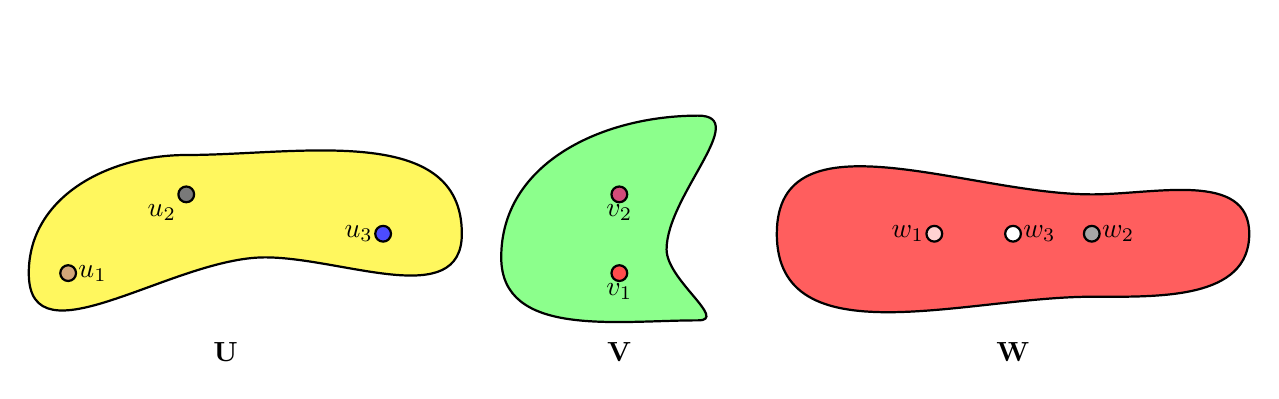
\begin{tikzpicture}[thick]
		\tikzstyle{edge} = [->, line width=1pt]
		%\tikzset{edge/.style = {->,> = latex'}}
		\node (v1) at (0,2) {};
		\node (v5) at (9,5) {};
		\node (v6) at (9,4.5) {};
		\node (v7) at (9,4) {};
		
		
		\node (v2) at (1.5,3) {};
		\node at (2,1) {$\bf \textcolor{black}{U}$};
		\node (v3) at (4,2.5) {};
		\node (v4) at (7,2) {};
		\node (v5) at (7,3) {};
		\node at (7,1) {$\bf \textcolor{black}{V}$};
		\node at (12,1) {$\bf \textcolor{black}{W}$};
		\node (u0) at (11,2.5) {};
		\node (u1) at (12,2.5) {};
		\node (u2) at (13,2.5) {};
	
		
		\begin{scope}[fill opacity=0.9]
			\filldraw[fill=yellow!70] ($(v1)+(-0.5,0)$) 
			to[out=90,in=180] ($(v2) + (0,0.5)$) 
			to[out=0,in=90] ($(v3) + (1,0)$)
			to[out=270,in=0] ($(v2) + (1,-0.8)$)
			to[out=180,in=270] ($(v1)+(-0.5,0)$);
			
			
			
			\filldraw[fill=green!50] ($(v4)+(-1.5,0.2)$)
			to[out=90,in=180] ($(v4)+(1,2)$)
			to[out=0,in=90] ($(v4)+(0.6,0.3)$)
			to[out=270,in=0] ($(v4)+(1,-0.6)$)
			to[out=180,in=270] ($(v4)+(-1.5,0.2)$);
			
			
			%	\begin{scope}
				%	\filldraw[fill opacity=0.9]
				\filldraw[fill=red!70] ($(u1)+(-3,0)$) 
				to[out=90,in=180] ($(u2) + (0,0.5)$) 
				to[out=0,in=90] ($(u0) + (4,0)$)
				to[out=270,in=0] ($(u2) + (0,-0.8)$)
				to[out=180,in=270] ($(u1)+(-3,0)$);
			\end{scope}
			
			
			\filldraw[fill=brown!70] (v1) circle (0.1) node [right] {$u_1$};
			\filldraw[fill=darkgray!70] (v2) circle (0.1) node [below left] {$u_2$};
			\filldraw[fill=blue!70] (v3) circle (0.1) node [left] {$u_3$};
			\filldraw[fill=red!70] (v4) circle (0.1) node [below] {$v_1$};
			\filldraw[fill=purple!70] (v5) circle (0.1) node [below] {$v_2$};
			\filldraw[fill=white!70] (u1) circle (0.1) node [right] {$w_3$};
			\filldraw[fill=gray!70] (u2) circle (0.1) node [right] {$w_2$};
			\filldraw[fill=pink!70] (u0) circle (0.1) node [left] {$w_1$};
		\end{tikzpicture}
		\caption{\label{fig:M1} An example of a {\em partition matroid} $(E,\cI)$, which  can be efficiently encoded. The ground set is $E = \{u_1,u_2,u_3,v_1,v_2,w_1,w_2,w_3\}$, partitioned into three sets: $U,V,W$. The independent sets are all subsets of $E$ containing at most one element from $U,V$, and $W$; that is, $\cI = \{S \subseteq E~|~\forall X \in \{U,V,W\}: |S \cap X| \leq 1\}$. A simple efficient encoding of $(E,\cI)$ is $I = (E,U,V,W)$. %Clearly, $|I|$ is polynomial in $E$; in addition, 
			Membership can be decided efficiently given $I$, by checking the feasibility
			of a given set $S$ w.r.t. $U,V$ and $W$.} 
	\end{figure}

Recall that \Cref{thm:emb} asserts that oracle-EMB does not admit a pseudo-polynomial time algorithm. However, %Fully PTAS,
 this does not rule out that hypothetically, for every matroid decoder $f$ there is a pseudo-polynomial time algorithm  %Fully PTAS 
 for $f$-decoded EMB. The next result excludes this option. %Our objective is to rule out this option. 

\begin{theorem}
	\label{thm:embA}
		Assuming $\textnormal{P} \neq \textnormal{NP}$, there is a matroid decoder $f$ such that there is no algorithm  for $f$-\textnormal{decoded EMB} that for any  $f$-\textnormal{decoded EMB} instance $U =(I,c,T)$, where $n = \left|E_{f(I)}\right|+1$ and $m = c\left(E_{f(I)}\right) +1$, runs in time $ (n \cdot(T+2) \cdot m)^{O(1)}$. 
\end{theorem}

	
	
The proof of \Cref{thm:embA} is given towards the end of this section. Analogously to our hardness result for oracle MOL problems, we use \Cref{thm:embA} to give a hardness result for an encoded version of MOL problems. For every matroid decoder $f$ and every $P \in \cP$, we define a variant of the $P$-{\sc matroid optimization with a linear constraint ($P$-MOL)} problem %BM, EMI, CMB and KCM 
	in which the matroid is given via an arbitrary bit-string which a matroid decoder $f$ decodes into a matroid. 
	Formally, let $P \in \cP$, where $P = (\opt,\cF,\triangleleft)$, be the parameters of the $P$-MOL problem. For a matroid decoder $f$, we define the $f$-decoded $P$-MOL problem as follows.  
	
		\problem{ {\sc $f$-decoded $P$-matroid optimization with a linear constraint} (f-decoded $P$-MOL)}{
		{\bf Decoder} & $f:\{0,1\}^* \rightarrow 2^\mathbb{N} \times 2^{2^{\mathbb{N}}}$ is a matroid decoder.\\
		{\bf Instance} &   $(I,v,w,L)$, where $I \in \{0,1\}^*$,  $v:E_{f(I)} \rightarrow \mathbb{R}_{\geq 0}$, $w:E_{f(I)} \rightarrow\mathbb{R}_{\geq 0}$, $L \in \mathbb{R}_{\geq 0}$. \\
	%	{\bf Matroid} & $\cm_{f(I)} = \left(E_{f(I)},\cI_{ f(I)}\right)$.\\ 
		{\bf Objective} & $\opt~ v(S) \text{ s.t. } S \in \cF\left(f(I)\right),~  w(S) \triangleleft L$.
	}
	
	For example, consider the encoded version of the %{\sc budgeted matroid independent set (BM)} (or, 
	$P$-MOL for $P = (\max,\IS,\leq)$ with the matroid decoder $f_{\textsf{u}}$ that decodes uniform matroids. %In this variant, the matroid is decoded by a matroid decoder $f_{\textsf{u}}$ from a bit  $I = (E,k) \in \{0,1\}^*$. 
	An instance of the $f_{\textsf{u}}$-decoded $P$-MOL problem is a tuple $U = (I,v,w,L)$ where $I = (E,k)$ is a bit-string used for extracting the uniform matroid $f_{\textsf{u}}(I) = (E,\cI)$ such that $\cI = \{S \subseteq E~|~|S| \leq k\}$, $v$ is the value function, $w$ is the weight function, and $L$ is the bound. %By the definition of $f_{\textsf{u}}$, a 
	A {\em solution} of $U$ is $S \subseteq E$ such that $|S| \leq k$ and $w(S) \leq L$; the goal is to find a solution $S$ of maximum value $v(S)$. This problem is widely known as {\sc knapsack with cardinality constraint}.  
	
	%We will define similar variants of EMI, CMB and KCM later.
	%Hypothetically, while 
	%As for EMB, even though \Cref{thm:main} rules out a Fully PTAS for every non-trivial oracle MOL problem, this hardness result does not necessarily hold for the encoded variants of MOL problems. 
	Recall that $\cQ = \cP \setminus \{(\min,\IS,\leq)\}$ is the set of parameters for non-trivial MOL problems. Using the hardness of $f$-decoded, for some matroid decoder $f$ (details on $f$ are given towards the end of the section), we show the hardness of the $f$-decoded  variant of all non-trivial MOL problems.
	
	

	 \begin{theorem}
	 	\label{thm:mainA}
	 	Assuming $\textnormal{P} \neq \textnormal{NP}$, for any $P \in \cQ$ there is a matroid decoder $f$ such that there is no \textnormal{Fully PTAS} for $f$-\textnormal{decoded} $P$-\textnormal{MOL}. 
	 \end{theorem}
	 
	 In the remainder of this section, we prove \Cref{thm:embA} and  \Cref{thm:mainA}. The matroid decoder used in our proofs decodes a subclass of the $\Pi$-matroid family (see \Cref{sec:Pi}), in which the secret family $\Pi$ consists of the solutions for a  {\sc boolean satisfiability problem (SAT)} instance. 
	
	
	In a SAT instance $A = (V,\bar{V},\cC)$ with $n \in \mathbb{N}$ variables (in a slightly simplified notation), we are given a set $V = \{v_1, \ldots,v_n\}$ of variables, their negations $\bar{V} = \{\bar{v}_1,\ldots, \bar{v}_n\}$, and a set $\cC \subseteq 2^{V \cup \bar{V}}$ of clauses. 
	The goal is to decide if there is a set $S \subseteq [n]$ %an assignment $\sigma:V \rightarrow \{0,1\}$ 
	satisfying that for all $C \in \cC$ there is $i \in [n]$ such that one of the following holds.   \begin{itemize}
		\item $v_i \in C$ and $i \in S$.
		\item $\bar{v}_i \in C$ and $i \notin S$. 
	\end{itemize} Such a set $S$ is called a {\em solution} of $A$; let $\mathcal{S}(A)$ be the set of solutions of a SAT instance $A$. In addition, let $n(A) = n$ be the number of variables in the instance $A$. 
	The family of SAT-matroids is the subfamily of $\Pi$-matroids where $\Pi = \mathcal{S}(A)$ for some SAT instance $A$ (for the notation and definition of $\Pi$-matroids, see \Cref{def:Matroid}). Specifically, 
	%\footnote{Recall that $\Pi$-matroids are defined in \Cref{sec:Pi}.} Formally, 
	
	\begin{definition}
		\label{def:SATmatroid}
		%	Let $n,k,\alpha \in \mathbb{N}_{>0}$, and 
		Let $A$ be a \textnormal{SAT} instance, $k \in \left[n(A)\right]$, and $\alpha \in \left[  {n(A)}^{2}\right]$. Define the {\bf SAT-matroid} on $A,k,\alpha$ as $M_{n(A),k,\alpha}(\mathcal{S}(A)) = \left(\left[n(A)\right],\cI_{n(A),k,\alpha}(\mathcal{S}(A))\right)$. 
	\end{definition}
	We show below that SAT-matroids can be  encoded efficiently. %\footnote{Technically, we also restrict $k$ and $\alpha$ to be small w.r.t. $n$.} 
	For every $I \in \{0,1\}^*$, we interpret $I$ as $I = (A,k,\alpha)$, where $A$ is a \textnormal{SAT} instance, $k \in \left[n(A) \right]$, and $\alpha \in \left[ {n(A)}^2 \right]$; w.l.o.g., we may assume that every $I = (A,k,\alpha) \in \{0,1\}^*$ can be interpreted in that manner; moreover, we can assume that $n(A) \leq |A|$, where $|A|$ is the encoding size of $A$. The following definition defines a matroid decoder that decodes SAT-matroids from a bit-string. %Additionally, for simplicity we use $A_I=A$, $n_I = n(A)$, $k_I = k$, and $\alpha_I = \alpha$ for $I = (A,k,\alpha)$. 
	\begin{definition}
		\label{def:SATencoder}
		Define the {\em SAT-decoder}  as the function $f_{\textnormal{SAT}}:\{0,1\}^* \rightarrow 2^\mathbb{N} \times 2^{2^{\mathbb{N}}}$ such that for all $I = (A,k,\alpha) \in \{0,1\}^*$ it holds that $f_{\textnormal{SAT}}(I) = M_{n(A),k,\alpha}(\mathcal{S}(A))$. 
	\end{definition}
	In the next result, we show that the SAT-decoder $\fs$ is indeed a  matroid decoder.
	\begin{lemma}
		\label{lem:encodable}
		%The \textnormal{SAT-decoder} 
		$\fs$ is a matroid decoder such that $|I| = |A|^{O(1)}$ for every $I=(A,k,\alpha) \in \{0,1\}^*$. 
	\end{lemma}
	Recall the sets  $\mathcal{J}_{n,k}$,  $\mathcal{K}_{n,k,\alpha}$, $\mathcal{L}_{n,k,\alpha}(\Pi)$ and $\cI_{n,k,\alpha}(\Pi)$ were defined in  \Cref{def:Matroid}.
	\begin{proof} %[Proof of 
		We first show that $\fs$ is a matroid decoder. %; otherwise, $f$ returns the trivial matroid $(\emptyset,\{\emptyset\})$. 
		%
		%Let $n,k,\alpha \in \mathbb{N}_{>0}$, and let $A = (V,\bar{V},\cC)$ be a \textnormal{SAT} instance with $n$ variables. We show that $M_{n,k,\alpha}(\mathcal{S}(A))$ is an encodable matroid. 
		%
		For all $I = (A,k,\alpha) \in \{0,1\}^*$  it holds that $\mathcal{S}(A) \subseteq 2^{\left[n(A)\right]}$; thus, by \Cref{lem:1} it holds that $f_{\textnormal{SAT}}(I)$ returns a matroid. Moreover, for all $I = (A,k,\alpha) \in \{0,1\}^*$ it holds that $k,\alpha = {n(A)}^{O(1)}$ and $n(A) \leq |A|$ by our encoding; hence, $|I| = |A|^{O(1)}$.  It remains to prove that $\fs$ satisfies \Cref{cond:1,cond:2} in \Cref{def:encode}.
		\begin{enumerate}
			\item  	\Cref{cond:1}. Given $I = (A,k,\alpha) \in \{0,1\}^*$, we can compute $E_{f_{\textnormal{SAT}}(I)} = \left[n(A)\right]$ in time $|I|^{O(1)}$ by identifying the number of variables (i.e., $n(A)$) in $A$. 
			\item 		\Cref{cond:2}. Let $I = (A,k,\alpha) \in \{0,1\}^*$ and let $n = n(A)$; we show that we can decide membership in the matroid $\fs(I)$ in time $\io$.  %and recall that  %and let $I = (A,k,\alpha)$. %If $f(I) = (\emptyset, \{\emptyset\})$ then trivially we can decide if $S \subseteq \emptyset$ belongs to $\{\emptyset\}$ in time $\io$. Otherwise, 
			% there are $k,\alpha \in \mathbb{N}_{>0}$, and a SAT instance $A$ such that 
			%	$f_{\textnormal{SAT}}(I) = M_{n_I,k_I,\alpha_I}(\mathcal{S}(A_I))$. 
			For every $S \subseteq \left[n\right]$ we can compute $|S|$ and $\textsf{sum}(S)$ in time $|I|^{O(1)}$. Thus, validating if $S \in \mathcal{J}_{n,k}$ or $S \in \mathcal{K}_{n,k,\alpha}$ can be computed in time $\io$ regardless of $\mathcal{S}(A)$. In addition, %SAT is known to be in NP; thus, 
			deciding if $S \in \mathcal{S}(A)$ can be computed in time $|A|^{O(1)} = |I|^{O(1)}$ by confirming that all clauses are satisfied. Thus, by \eqref{eq:1} we can decide if $S \in \mathcal{L}_{n,k,\alpha}(\mathcal{S}(A))$. Overall, deciding whether $S \in \mathcal{J}_{n,k}$, $S \in \mathcal{K}_{n,k,\alpha}$, or $S \in \mathcal{L}_{n,k,\alpha}(\mathcal{S}(A))$ can be computed in time $|I|^{O(1)}$. By the above and \eqref{eq:1}, we can compute in time $\io$ correctly if a set $S$ belongs to $\cI_{\fs (I)} = \cI_{n,k,\alpha}(\mathcal{S}(A))$. 
		\end{enumerate}
		Thus, $\fs$ is a matroid decoder by \Cref{def:encode}, which gives the statement of the lemma.  %, satisfying that $|I| = |A|^{O(1)}$ for every $I=(A,k,\alpha) \in \{0,1\}^*$. . 
	\end{proof} 
	
	

	
	
	
	We will use an algorithm for $f$-decoded EMB to obtain an algorithm for SAT. To this end, consider the following family of {\em structured } $\fs$-decoded EMB instances.
		
		
											\begin{definition}
			\label{def:problemE}
			An $\fs$-{\sc decoded EMB} instance $(I,c,T)$, where $I = (A,k,\alpha)$ is called {\em structured} if  $\alpha \in \left[ {n(A)}^2 \right]$, $T = \alpha$, and $c: \left[ n(A) \right] \rightarrow \mathbb{N}$ such that for all $i \in \left[ n(A) \right]$ it holds that $c(i) = i$ %\textnormal{\textsf{sum}}(S)$.  
		\end{definition}
		
		
		The next observation immediately follows from the definition of structured $\fs$-decoded EMB instances and SAT-matroids. 
		
		\begin{observation}
			\label{obs:YesNoD}
			%For every $n,k,\alpha \in \mathbb{N}_{>0}$, $\Pi \subseteq 2^{[n]}$ 
			for any structured $\fs$-{\sc decoded EMB} instance $U = (I,c,T)$, where $I = (A,k,\alpha)$, and $S \subseteq \left[ n(A)\right]$, it holds that: $S$ is a solution for $U$ if and only if $S \in \mathcal{S}(A)$, $|S| = k$, and $\textnormal{\textsf{sum}}(S) = c(S) = \alpha$. 
		\end{observation}
		
		%The following hardness result, 
		We show that given a polynomial algorithm that decides structured $\fs$-decoded EMB instances, we can decide SAT. This result easily imply \Cref{thm:embA} as shown afterwards.  
		
%		\begin{definition}
%			An instance $s$
%		\end{definition}

		\begin{lemma}
				\label{lem:SAT}
				Assuming $\textnormal{P} \neq \textnormal{NP}$, there no algorithm that decides every $\fs$-decoded \textnormal{EMB} structured instance $(I,c,T)$ in time $\io$. 
			\end{lemma}
	\begin{proof}
	
	Assume that $\textnormal{P} \neq \textnormal{NP}$ and assume towards a contradiction that there is an algorithm $\cA$ that decides every $\fs$-decoded EMB structured instance $(I,c,T)$ in time $\io$. We describe the following algorithm $\cB$ which decides SAT using $\cA$. Let $A$ be a SAT instance and let $n = n(A)$. 
	%We describe the following algorithm $\cB$ which decides $(A,k)$. 
	\begin{enumerate}
		\item 	For every $k \in \left[n\right]$ and $\alpha \in \left[n^2\right]$, let $I_{k,\alpha} = (A,k,\alpha)$; execute $\cA$ on the structured instance $U_{k,\alpha} = (I_{k,\alpha},c,\alpha)$. %such that $f_{\textnormal{SAT}}(I_{\alpha}) = M_{n,k,\alpha}(\mathcal{S}(A))$. 
		\item  If $\emptyset$ is a solution for $A$,  return ``yes" on $A$. 
		\item If there are $k \in \left[n\right]$ and $\alpha \in \left[n^2\right]$ such that $\cA$ returns ``yes" on $U_{k,\alpha}$, %is a ``yes"-instance or $(ii)$ $\emptyset$ is a solution for $A$, %decides that $\mathcal{L}_{n,k,\alpha}(\mathcal{S}(A)) \neq \emptyset$, %yields a solution $S \in \mathcal{S}(A)$ 
	 return ``yes" on $A$. %has a solution.
	 \item Otherwise, return ``no" on $A$. %does not have a solution.
	\end{enumerate}
	To show that $\cB$ decides SAT, consider the following cases. 
	\begin{itemize}
		\item $A$ is a ``yes"-instance. Then, there is a solution $S \in \mathcal{S}(A)$. If $\emptyset \in \mathcal{S}(A)$ then $\cB$ returns ``yes" on $A$. Otherwise, there are $k \in [n]$, $\alpha \in \left[n^2\right]$, and a solution $S \in \mathcal{S}(A)$ such that $|S| = k$ and $ \textnormal{\textsf{sum}}(S) = \alpha$. Since $U_{k,\alpha}$ is structured, we have $c(S) = \alpha$; therefore, $S$ is a solution for $U_{k,\alpha}$ by \Cref{obs:YesNoD}. Consequently, $\cA$ returns ``yes" on $U_{k,\alpha}$; hence, $\cB$ returns ``yes" on $A$.  
		
	
		
		\item $A$ is a ``no"-instance. Then, $\mathcal{S}(A) = \emptyset$. %In particular, $\emptyset \notin \mathcal{S}(A)$. %for every $k \in [n]$ and $\alpha \in \left[ n^2\right]$ there is no solution for instance $I_{A,k,\alpha}$. 
		Assume towards a contradiction that $\cB$ returns ``yes" on $A$. Thus, since $\emptyset \notin \mathcal{S}(A)$, there are $k \in [n]$ and $\alpha \in \left[ n^2\right]$ such that $\cA$ returns ``yes" on $U_{k,\alpha}$, implying that there is a solution $S$ for $U_{k,\alpha}$. Since $U_{k,\alpha}$ is structured, by \Cref{obs:YesNoD} it holds that $S \in \mathcal{S}(A)$. 
		This is a contradiction that $\mathcal{S}(A) = \emptyset$. Thus, $\cB$ returns ``no" on $A$. 
	\end{itemize} 
	Hence, $\cB$ decides the SAT instance $A$ correctly. We analyze the running time below.  
	
	 By our encoding, it holds that $n \leq |A|$ as $A$ contains $n$ distinct variables. In addition, observe that the identity function $c:[n] \rightarrow [n]$ can be encoded using at most $n \cdot \log (n)$ bits (this is the weight function of every structured instance $U_{k,\alpha}$ constructed in the algorithm, for $k \in [n]$ and $\alpha \in \left[n^2\right]$). Then, for all $k \in [n]$ and $\alpha \in \left[ n^2\right]$ observe that the encoding of the instance $U_{k,\alpha}$ satisfies: $$|U_{k,\alpha}| = |A|+k+\alpha+n \cdot \log (n) \leq |A|+n+n^2 +n \cdot \log (n)= O\left(|A|^2\right).$$ %The first equality holds since the function $c$ does not need to be encoded as it simply the identity function for structured instances. 
	 Moreover, the number of iterations (i.e., the number of distinct options for the parameters $k,\alpha$) is bounded by $n \cdot n^2 = n^3 = O(|A|^3)$. Thus, the running time of each iteration is bounded by $|U_{k,\alpha}|^{O(1)} = |A|^{O(1)}$ by the running time guarantee of $\cA$. Therefore, our algorithm decides SAT in time $|A|^{O(1)}$. Since SAT is known to be NP-Hard (see, e.g., \cite{garey1997computers} for more details), we reach a contradiction to the existence of $\cA$. %unless $\textnormal{P} = \textnormal{NP}$ such an algorithm $\cA$ cannot exist. 
\end{proof}

From the above result, the hardness of the more general $\fs$-decoded EMB easily follows. As an immediate corollary, \Cref{thm:embD} gives the proof of \Cref{thm:embA}. 

	\begin{restatable}{theorem}{thmembD}
	\label{thm:embD}
	Assuming $\textnormal{P} \neq \textnormal{NP}$, there is no algorithm  for $\fs$-decoded \textnormal{EMB} that runs in time $ (n \cdot(T+2) \cdot m)^{O(1)}$, for any  $\fs$-decoded \textnormal{EMB} instance $U =(I,c,T)$ where $n = \left|E_{\fs(I)}\right|+1$ and $m = c\left(E_{\fs(I)}\right) +1$. 
\end{restatable}

\begin{proof}
	Let $U = (I,c,T)$ be a structured $\fs$-decoded EMB instance and let $I = (A,k,\alpha)$. Recall that by our encoding it holds that $|I| \geq |A| \geq n(A)$. Thus, %; let $n = |E_{f(I)}|+1$ and $m = c(E_{f(I)})+1$. 
	since $U$ is structured, it follows that  $\left|E_{\fs(I)}\right| = n(A) \leq |I|$ and 
	$$c\left(E_{\fs(I)}\right) = \textsf{sum}\left(\left[n(A)\right]\right) \leq \frac{n(A) \cdot (n(A)+1)}{2} = O\left(|I|^2\right).$$
	Thus, by the above, an algorithm $\cA$ that decides every $\fs$-EMB  instance $(I',c',T')$ in time $(n' \cdot(T'+2) \cdot m')^{O(1)}$, where  $n' = |E_{\fs(I')}|+1$ and $m' = c\left(E_{\fs(I)}\right) +1$, in particular decides $U$ in time $\io$. As $U$ is an arbitrary structured instance, unless $\textnormal{P} = \textnormal{NP}$, by \Cref{lem:SAT} such an algorithm $\cA$ cannot exist.  
\end{proof}

%We can finally prove \Cref{thm:mainD}. 
%\thmMainD*

	Finally, %we use the SAT-decoder to 
	we show that %there is an $f$-BM problem which does not have 
the variants of non-trivial matroid optimization with a linear constraint (MOL) problems, in which the decoding is performed by the SAT-decoder $\fs$, do not admit Fully PTAS under the standard assumption $\textnormal{P} \neq \textnormal{NP}$.   The proof is similar to the proof of \Cref{thm:main} in \Cref{sec:tight_absolute}. \Cref{thm:mainD} directly gives the proof of \Cref{thm:mainA}.

\begin{restatable}{lemma}{thmMainD}
	\label{thm:mainD}
	Assuming $\textnormal{P} \neq \textnormal{NP}$, for any $P \in \cQ$ there is no \textnormal{Fully PTAS} for $\fs$-\textnormal{decoded} $P$-\textnormal{MOL}. 
\end{restatable}

\begin{proof}
	%Let $P \in \cQ$ be a non-trivial MOL problem. 
	Assume that $\textnormal{P} \neq \textnormal{NP}$ and assume towards a contradiction that there is a Fully PTAS $\cA$ for $\fs$-decoded $P$-MOL. We use $\cA$ to decide $\fs$-decoded EMB. Let $U = (I,c,T)$  be an $\fs$-decoded EMB instance. %let $n = |E|+1$ and let $m = c(E)+1$; observe that $n,m \neq 0$. C
	Consider the following algorithm $\cB$ that decides $U$. In the algorithm, we use the reduction described in \Cref{def:reduction} and an error parameter defined in \eqref{eq:epsI}. 
	\begin{enumerate}
		\item Construct the $\fs$-decoded $P$-MOL instance $X = (I,v_J,w_{J,P},L_{J,P})$, where \newline $J = \left(E_{\fs(I)},\cI_{\fs (I)},c,T\right)$ is an EMB instance.\label{step:1D} 
		\item 
		Execute $\cA$ with the input $X$ and $\eps_J$ (see \eqref{eq:epsI}). \label{step:2D} 
		\item If $\cA$ returns ``no" on $X$: Return ``no" on $U$. %does not have a solution. \label{step:3D} 
		\item Otherwise, let $S \leftarrow \cA(X,\eps_J)$ be the returned solution by $\cA$.\label{step:4D} 
		\item Return ``yes" on $U$ %has a solution 
		if and only if $v_J(S) = H_J \cdot k_J+T$. \label{step:5D} 
	\end{enumerate}
	
	Observe that $U,J$ share the same matroid, weight function, and target value; the only difference between them is the representation of the matroid, that is encoded in $U$ while in $J$ the representation of the matroid is not specified. Similarly, $X$ and $R_P(J)$ also share the same matroid, value function, weight function, and bound; the only difference between them is that $X$ gives a concrete encoding of the matroid.  
	
	Let $n = |E|+1$ and let $m = c(E)+1$. Note that $X$ can be trivially constructed from $U$ in time $\left(n \cdot (T+2) \cdot m\right)^{O(1)}$ by \Cref{def:reduction}. % moreover, in time $\left(n \cdot (T+2) \cdot m\right)^{O(1)}$ we can compute the instance $X$ from $J$. %because $\frac{1}{\eps} = \left(n \cdot (T+1)\cdot m\right)^{O(1)}$; 
	Thus, the running time of $\cB$ on $U$ is $\left(n \cdot (T+2) \cdot m\right)^{O(1)}$, since $\cA$ is a Fully PTAS for $\fs$-decoded $P$-MOL and by the selection of the error parameter  $\eps_J$ in \eqref{eq:epsI}. %For the correctness,
	We now show correctness. %For the 
	
	
	\begin{itemize}
		\item If $\cB$ returns ``yes" on $U$. %has a solution. 
		Then, Step 4 of the algorithm computes a solution $S$ for $X$ satisfying $v_J(S) = H_J \cdot k_J+T$. Clearly, $S$ is a solution for $R_P(J)$ as well. By \Cref{thm:H}, %since $S$ is a solution for $R_{P}(I)$ such that $v_I(S) = H_I \cdot k_I+T$ it also holds that 
		$S$ is also a solution for $J$. As $J$ and $U$ share the same matroid, weight function, and target value, we conclude that $S$ is a solution for $U$. Therefore, $U$ is a ``yes"-instance.     
		
		
		\item If $U$ is a ``yes"-instance. Then, $J$ has a solution. Therefore, by \Cref{thm:H} it holds that $R_P(J)$ has a solution, which implies that $X$ has a solution. Thus, since $\cA$ is a Fully PTAS for $\fs$-decoded $P$-MOL, $\cA$ returns a $(1+\eps_J)$-approximate solution $S$ for $X$; clearly, $S$ is also a $(1+\eps_J)$-approximate solution for $R_P(J)$. %Thus, $S$ is a $(1+\eps_J)$-approximation for $R_P(J)$. 
		Then, by \Cref{thm:H} it follows that $v_J(S) = H_J \cdot k_J+T$. Thus, $\cB$ returns ``yes" on $U$.
	\end{itemize}  Hence, $\cB$ decides $\fs$-decoded EMB in time $\left(n \cdot (T+2) \cdot m\right)^{O(1)}$, contradicting \Cref{thm:embD}.  
\end{proof}


	
	

	

%		  
\label{sec:NPhard}
\subsection{Budgeted Matroid Independent Set}

\label{sec:bm_np}


\lemsatbm*

%\begin{proof}
%	We use a reduction from the SAT-matroid problem. Let $I \in \{0,1\}^*$ be a SAT-matroid instance; for simplicity, let $A = A_I, n = n(A), k = k_I$, and $\alpha = \alpha_I$.  
%	%
%	%If $k \notin \mathbb{N}_{>0}$, $\alpha \notin \left[ n^2 \right]$, or $A$ is not a SAT instance with $n$ variables, we can verify it in time $\io$ and decide correctly the SAT-matroid instance $I$ in time $|I|^{O(1)}$. Thus, for the following, assume that $n,k \in \mathbb{N}_{>0}, \alpha \in \left[ n^2 \right]$,  and that $A$ is a SAT instance with $n$ variables. %$I = \left(n,k,\alpha,\mm\right)$ be a $\Pi$-matroid instance. 
%	We define the $\fs$-BM instance $$U = (I,w_{n},w_{n},B_{n,k,\alpha}).$$ Note that $\fs (I) = M_{n,k,\alpha}(\mathcal{S}(A))$ by \Cref{def:SATencoder}. %is an encodable matroid by \Cref{lem:encodable}; 
%	Moreover, by \Cref{lem:encodable}, \eqref{eq:w}, and \eqref{eq:B} it follows that $U$ can be constructed from $I$ in time $|I|^{O(1)}$.   
%	%
%	%For all $S \subseteq [n]$ it holds that $w_{n}(S) \in \mathbb{N}$ and that $$\OPT \left( U\right) \leq n \cdot \max_{i \in [n]} p(i) = n^2 = \left| U \right|^{O(1)}.$$  
%	%
%	To show that $U$ is a scaled $\fs$-BM instance, observe that for all $S \subseteq [n]$ it holds that $w_{n}(S) \in \mathbb{N}$ and that $\OPT \left( U\right) = \left| U \right|^{O(1)}$ by \Cref{lem:OPTu}. Therefore, if $\fs$-BM has an FPTAS, by \Cref{lem:FPTAStoEXACT} there is an exact algorithm $\cA$ that finds in time $\left| U \right|^{O(1)} = \io$ an optimal solution for $U$. Clearly, $\OPT(U) \leq B_{n,k,\alpha}$ since the profit and the cost of each element are the same. Therefore, by \Cref{cor:iff} the algorithm $\cA$ on instance $U$ returns a solution for $U$ with profit $B_{n,k,\alpha}$ if and only if $I$ has a solution. %Hence, we can decide $I$ by computing $\cA$ on $U$ and return that $I$ has a solution if and only if $\cA$ returns that $U$ has a solution for $U$ with profit $B_{n,k,\alpha}$Thus, $\cA$ is a polynomial algorithm that decides the SAT-matroid problem, 
%	Hence, by computing $\cA$ on $U$ and getting a solution $S$, we can decide correctly $I$ by returning that $I$ has a solution if and only if $w_n(S) = B_{n,k,\alpha}$. The above algorithm decides the SAT-matroid problem, which is impossible by \Cref{cor:Strong}, unless P=NP. 
%\end{proof}



\begin{proof}
	
	
	
	%	\noindent{\bf Proof of \Cref{lem:hard}:}
	Assume that P$\neq$NP and assume towards a contradiction that there is a Fully PTAS $\cA$ for $\fs$-BM. We use $\cA$ to decide the $\Pi$-matroid problem.  Let $I \in \{0,1\}^*$ be a SAT-matroid instance. Consider the following algorithm $\cB$ that decides $I$. For simplicity, let $A = A_I, n = n(A), k = k_I$, and $\alpha = \alpha_I$.  %let $n = n_I,k = k_I,\alpha = \alpha_I$, and $A = A_I$. 
	\begin{enumerate}
		\item Construct the $f_{\textnormal{SAT}}$-BM instance $%U_{n,k,\alpha}(\Pi) 
		U= (I,w_{n},w_{n},B_{n,k,\alpha})$. Note that $\fs (I) = M_{n,k,\alpha}(\mathcal{S}(A))$ by \Cref{def:SATencoder}. %is an encodable matroid by \Cref{lem:encodable}; 
		
		
		%; note that the elements of $U$ are $[n] = \{1,\ldots, n \}$, the independent sets are the independent sets of the $\Pi$-matroid $\mm$ (i.e., $\cI_{n,k,\alpha}(\Pi)$), the standard weight function $w_n$ is both the profit and the cost function, and the budget is simply the standard budget with parameters $n,k,\alpha$. %Let $U = U_{n,k,\alpha}(\Pi)$ for simplicity.
		\item Define $\eps = \frac{1}{6 \cdot n^3}$ and compute $\cA$ on $U$ and $\eps$; let $S$ be the returned solution.  
		\item Return that $I$ has a solution if and only if $w_n(S) = B_{n,k,\alpha}$. 
	\end{enumerate}
	
By \Cref{lem:encodable}, \eqref{eq:w}, and \eqref{eq:B} it follows that $U$ can be constructed from $I$ in time $|I|^{O(1)}$.   In addition, %Note that $U$ can be constructed from $I$ in time $\io$ and that 
$\frac{1}{\eps} = n^{O(1)} =|I|^{O(1)}$; thus, the running time of $\cB$ on $I$ is $|I|^{O(1)}$, since $\cA$ is an FPTAS. We now show correctness. %For the correctness, %we show that $\cB$ returns that $I$ has a solution if and only if $I$ indeed has a solution. 
	\begin{itemize}
		\item If $\cB$ returns that $I$ has a solution then $w_n(S) = B_{n,k,\alpha}$; since $S$ is a solution for $U$ it also holds that $S \in \cI_{\fs (I)} = \cI_{n,k,\alpha}(\mathcal{S}(A))$. Thus, by \Cref{cor:iff} it holds that $I$ has a solution.  
		\item If $I$ has a solution then there is $T \in \mathcal{L}_{n,k,\alpha}(\mathcal{S}(A))$; thus, by  \Cref{cor:iff} it follows that $w_n(T) = B_{n,k,\alpha}$ implying that $T$ is a solution for $U$.  Therefore, %w.p. at least $\frac{1}{2}$: 
		\begin{equation}
			\label{eq:sOPT}
			B_{n,k,\alpha} \geq \OPT(U) \geq w_n(S) \geq (1-\eps) \cdot w_n(T) \geq  w_n(T)-\frac{1}{6 \cdot n^3} \cdot 3 \cdot n^3 = B_{n,k,\alpha}-\frac{1}{2}.
		\end{equation} 	The first inequality holds since %$w_n(T) = B_{n,k,\alpha}$. In addition, $\OPT(U) \leq B_{n,k,\alpha}$ because 
		the profit and the cost of each element are the same, and the cost of a solution cannot exceed the budget. The third inequality follows because $S,T$ are solutions for $U$, and $S$ is computed by an FPTAS with the parameter $\eps$. The fourth inequality follows from \Cref{lem:OPTu} and by the selection of $\eps$. Observe that the value of $S$ is an integer by \eqref{eq:w}; thus, by \eqref{eq:sOPT}, %w.p. at least $\frac{1}{2}$ 
		it holds that $w_n(S) = B_{n,k,\alpha}$. Then, $\cB$ returns that $I$ has a solution.  
	\end{itemize}
%	Hence, %by computing $\cA$ on $U$ and getting a solution $S$, 
%	the algorithm $\cB$ is an solves the SAT matroid problem correctly. %if and only if $w_n(S) = \OPT(U)$, which holds w.p. at least $\frac{1}{2}$. 
Hence $\cB$ is %by returning that $I$ has a solution if and only if $w_n(S) = B_{n,k,\alpha}$. Thus, we 
	a polynomial time algorithm for the  SAT-matroid problem, contradicting \Cref{cor:Strong}. 
\end{proof}



\subsection{Exact Weight Matroid Independent Set}

Similarly to $f$-BM, we can define a variant of EMI for every matroid encoder $f$.

	\problem{ {\sc $f$-Exact Matroid Independent Set} ($f$-EMI)}{
	{\bf Encoder} & $f:\{0,1\}^* \rightarrow 2^{\mathbb{N}} \times 2^{2^{\mathbb{N}}}$ is a matroid encoder. \\
	{\bf Instance} &  $U =  (I,w,k,T)$, where $I \in \{0,1\}^*$, $w:E_{f(I)} \rightarrow \mathbb{N}$ gives the elements weights, $k\in \mathbb{N}$ is  the target cardinality, and $T \in \mathbb{N}$ is the target weight. \\
	{\bf Solution }& $S\in \cI_{f(I)}$ such that $|S|=k$ and $w(S)=T$.\\
{\bf Objective} & Decide if there exists a solution.
}



\begin{lemma}
	\label{lem:f-EMI}
	Unless \textnormal{W[1]=FPT}, for any computable function $f:\mathbb{N} \rightarrow \mathbb{N}$ there is no algorithm that decides \textnormal{EMI} in time $f(k) \cdot \left( T\cdot |I|\right)^{O(1)}$, where $|I|$ is the encoding size of the instance, $k$ is the target cardinality and $T$ is the target weight.
\end{lemma}
\begin{proof}
	Assume that \textnormal{W[1]}$\neq$\textnormal{FPT}. 
	Assume towards a contradiction that the statement of the lemma does not hold. Thus, there is a computable  function $f:\mathbb{N} \rightarrow \mathbb{N}$, and an algorithm $\cA$ that decides $\fs$-\textnormal{EMI} in time $f(k) \cdot {(T \cdot |I|)}^{O(1)}$. We use $\cA$ to decide the SAT-matroid problem. 
Let $I \in \{0,1\}^*$ be a SAT-matroid instance. Consider the following algorithm $\cB$ that decides $I$. For simplicity, let $A = A_I, n = n(A), k = k_I$, and $\alpha = \alpha_I$. Assume that $k \leq n$ or the instance can be trivially decided. 
	\begin{enumerate}
		\item Construct the $\fs$-EMI instance $%U_{n,k,\alpha}(\Pi) 
		U= (I,w_{n},k,B_{n,k,\alpha})$. Note that $\fs (I) = M_{n,k,\alpha}(\mathcal{S}(A))$ by \Cref{def:SATencoder}. %Let $U = U_{n,k,\alpha}(\Pi)$ for simplicity.
		\item %Define $\eps = \frac{1}{6 \cdot n^3}$ and 
		Compute $\cA$ on $U$. %and let $S$ be the returned solution.  
		\item Return that $I$ has a solution if and only if $\cA$ returns that $U$ has a solution.   %$w_n(S) = B_{n,k,\alpha}$. 
	\end{enumerate}
	To show $\cB$ indeed solves the SAT-matroid instance, consider the following cases. 
	\begin{itemize}
		\item If  $\cB$ returns that $I$ has a solution then $w_n(S) = B_{n,k,\alpha}$ and $S \in \cI_{\fs (I)} = \cI_{n,k,\alpha}(\mathcal{S}(A))$. Thus, by \Cref{cor:iff} it holds that $I$ has a solution.  
		\item If $I$ has a solution then there is $T \in \mathcal{L}_{n,k,\alpha}(\mathcal{S}(A))$; thus, by  \Cref{cor:iff} it follows that $w_n(T) = B_{n,k,\alpha}$. Also, by the definition of $\mathcal{L}_{n,k,\alpha}(\mathcal{S}(A))$ it holds that $|T|=k$.  Therefore $T$ is a solution of $U$. Therefore, $\cA$ returns that $U$ has a solution; thus, $\cB$ returns that $I$ has a solution. 
	\end{itemize}
It follows that $\cB$ is an algorithm for the SAT-matroid problem.

%	Note that $U$ can be constructed naively from $I$ in time $n+n \cdot (2n^2+n)+2n \cdot k+n^2 \leq 6 \cdot n^3$ (recall that the weights are encoded in unary and that $k \leq n$); thus, the running time of $\cB$ on $I$ is bounded by $6 \cdot n^3+f(k) \cdot n^{q} = f(k) \cdot n^{O(1)}$. 
	Note that $B_{n,k,\alpha} = 2k \cdot \textsf{sum}(n) \leq 2k \cdot n^2 \leq 2 \cdot n^3$ since $k \leq n$.  The instance $U$ can be trivially constructed in time $|I|^{O(1)}$, thus the overall running time of $\cB$ is $f(k)\cdot (2\cdot n^3\cdot |I|^{O(1)})^{O(1)} \leq f(k)\cdot |I|^{O(1)}$. That is, $\cB$ is a parameterized algorithm for the SAT-matroid problem, in contradiction to \Cref{lem:FPT}. Thus, the statement of the lemma holds.
\end{proof}

























\subsection{Constrained minimum Basis of a Matroid}

We proceed to define a variant of CMB in which the matroid is encoded as part of the instance.
\problem{ {\sc $f$-Constrained minimum Basis of a Matroid} ($f$-CMB)}{
	{\bf Encoder} & $f:\{0,1\}^* \rightarrow 2^{\mathbb{N}} \times 2^{2^{\mathbb{N}}}$ is a matroid encoder. \\
	{\bf Instance} &  
	$U = (I,c,w,B)$, where $I \in \{0,1\}^*$,  $c:E_{f(I)} \rightarrow \mathbb{N}$ is a cost function, $w:E_{f(I)} \rightarrow \mathbb{N}$ is a weight function and $B \in \mathbb{N}$ is a budget.\\
	{\bf Solution}& A basis $S \in \cI_{f(I)}, |S| = \max_{S' \in \cI_{f(I)}} |S'|$ such that $c(S) \leq B$.\\
	{\bf Objective} & Find a solution $S$ of $U$ with minimum weight $w(S)$.
	%	{\bf Model } &The independent sets $\cI$ is only accessible via a membership oracle; the encoding cost of the instance $U$ is the encoding cost of $(E,c,p,B)$, the instance without $\cI$.
}

\begin{lemma}
	\label{lem:CMB-NP}
	Unless \textnormal{P=NP}, there is no \textnormal{Fully PTAS} for $f_{\textnormal{SAT}}$-\textnormal{CMB}. 
	%If there is an algorithm for \textnormal{BM} in $X(n)$   
\end{lemma}
	\begin{proof}
		Assume that P$\neq$NP and assume towards a contradiction that there is a Fully PTAS $\cA$ for $f_{\textnormal{SAT}}$-CMB. We use $\cA$ to decide the SAT-matroid problem.  Let $I \in \{0,1\}^*$ be a SAT-matroid instance. Consider the following algorithm $\cB$ that decides $I$. For simplicity, let $A = A_I, n = n(A), k = k_I$, and $\alpha = \alpha_I$. 
	\begin{enumerate}
		\item Construct the $f_{\textnormal{SAT}}$-CMB instance $%U_{n,k,\alpha}(\Pi) 
		U= (I,c_n,w_{n},L_{n,k,\alpha})$. Note that $\fs (I) = M_{n,k,\alpha}(\mathcal{S}(A))$ by \Cref{def:SATencoder}.  %along with the membership oracle of $M_{n,k,\alpha}(\Pi)$; note that the elements of $U$ are $[n] = \{1,\ldots, n \}$, the independent sets are the independent sets of the $\Pi$-matroid $\mm$ (i.e., $\cI_{n,k,\alpha}(\Pi)$), the cost is the standard cost function, the weight is the standard weight function $w_n$, and the bound is the standard bound with parameters $n,k,\alpha$. %Let $U = U_{n,k,\alpha}(\Pi)$ for simplicity.
		\item Define $\eps = \frac{1}{6 \cdot n^3}$ and compute $\cA$ on $U$ and $\eps$; let $S$ be the returned solution.  
		\item Return that $I$ has a solution if and only if $w_n(S) = B_{n,k,\alpha}$. 
	\end{enumerate}
By \Cref{lem:encodable}, \eqref{eq:w}, and \eqref{eq:B} it follows that $U$ can be constructed from $I$ in time $|I|^{O(1)}$.   In addition, %Note that $U$ can be constructed from $I$ in time $\io$ and that 
$\frac{1}{\eps} =n^{O(1)} = |I|^{O(1)}$; thus, the running time of $\cB$ on $I$ is $|I|^{O(1)}$, since $\cA$ is an FPTAS. We now show correctness.
	%Note that $U$ can be constructed from $I$ in time $\io$ and that $\frac{1}{\eps} = |I|^{O(1)}$; thus, the running time of $\cB$ on $I$ is $|I|^{O(1)}$, since $\cA$ is a (randomized) FPTAS. We now show correctness. %For the correctness, %we show that $\cB$ returns that $I$ has a solution if and only if $I$ indeed has a solution. 
	\begin{itemize}
		\item If $\cB$ returns that $I$ has a solution. Then, $w_n(S) = B_{n,k,\alpha}$; since $S$ is a solution for $U$ it also holds that $S \in \cI_{\fs (I)} = \cI_{n,k,\alpha}(\mathcal{S}(A))$. Thus, by \Cref{cor:iff} it holds that $I$ has a solution.  
		\item If $I$ has a solution. Then, there is $T \in \mathcal{L}_{n,k,\alpha}(\mathcal{S}(A))$; thus, by  \Cref{cor:iff} it follows that $w_n(T) = B_{n,k,\alpha}$, which implies by \Cref{lemma:wl} that $c_n(T) \leq L_{n,k,\alpha}$. Then, since $T$ is a basis of $\mm$ (recall that $T \in \mathcal{L}_{n,k,\alpha}(\mathcal{S}(A))$), it follows that $T$ is a solution for $U$.  Hence,   
		\begin{equation}
			\label{eq:sOPTcmb}
			B_{n,k,\alpha} \leq \OPT(U) \leq w_n(S) \leq (1+\eps) \cdot w_n(T) \leq  w_n(T)+\frac{1}{6 \cdot n^3} \cdot 3 \cdot n^3 = B_{n,k,\alpha}+\frac{1}{2}.
		\end{equation} 	The first inequality follows from \Cref{lemma:wl} (note that $U$ has a solution since $T$ is a solution). %for every $S' \subseteq [n], |S'|<k$ it holds that $s$ every solution $S'$ for $U$ is a basis of $\mm$; thus, it follows that $w$ %$w_n(T) = B_{n,k,\alpha}$. In addition, $\OPT(U) \leq B_{n,k,\alpha}$ because 
		%	the profit and the cost of each element are the same, and the cost of a solution cannot exceed the budget. 
		The third inequality follows because $S,T$ are solutions for $U$, and $S$ is computed by an FPTAS with the parameter $\eps$. The fourth inequality follows from \Cref{lem:OPTu} and by the selection of $\eps$. Observe that the value of $S$ is an integer by \eqref{eq:w}; thus, by \eqref{eq:sOPTcmb}, %w.p. at least $\frac{1}{2}$ 
		it holds that $w_n(S) = B_{n,k,\alpha}$. Then, $\cB$ returns that $I$ has a solution.  
	\end{itemize}
	Hence, %by computing $\cA$ on $U$ and getting a solution $S$, 
	we decide $I$ correctly. %if and only if $w_n(S) = \OPT(U)$, which holds w.p. at least $\frac{1}{2}$. 
	It follows that $\cB$ is %by returning that $I$ has a solution if and only if $w_n(S) = B_{n,k,\alpha}$. Thus, we 
	a polynomial algorithm which decides the SAT-matroid problem, contradicting \Cref{cor:Strong}. 
\end{proof}























	\subsection{Knapsack Cover with a Matroid}

Finally, we define a variant of KCM with no oracle.

\problem{ {\sc $f$-Knapsack Cover with a Matroid} ($f$-KCM)}{
	{\bf Encoder} & $f:\{0,1\}^* \rightarrow 2^{\mathbb{N}} \times 2^{2^{\mathbb{N}}}$ is a matroid encoder. \\
	{\bf Instance} &  
	$U = (I,c,d,D)$, where $I \in \{0,1\}^*$,  $c:E_{f(I)} \rightarrow \mathbb{N}$ is a cost function, $d:E_{f(I)} \rightarrow \mathbb{N}$ is a size function, and $B \in \mathbb{N}$ is a demand.\\
	{\bf Solution}& $S \in \cI_{f(I)}$ such that $d(S) \geq D$.\\
	{\bf Objective} & Find a solution $S$ of $U$ with minimum cost $c(S)$.
	%	{\bf Model } &The independent sets $\cI$ is only accessible via a membership oracle; the encoding cost of the instance $U$ is the encoding cost of $(E,c,p,B)$, the instance without $\cI$.
}

\begin{lemma}
	\label{lem:KCM-NP}
	Unless \textnormal{P=NP}, there is no \textnormal{Fully PTAS} for $f_{\textnormal{SAT}}$-\textnormal{KCM}. 
	%If there is an algorithm for \textnormal{BM} in $X(n)$   
\end{lemma}

\begin{proof}
	Assume that P$\neq$NP and assume towards a contradiction that there is an FPTAS $\cA$ for $f_{\textnormal{SAT}}$-KCM. We use $\cA$ to decide the SAT-matroid problem. Let $I \in \{0,1\}^*$ be a SAT-matroid instance. Consider the following algorithm $\cB$ that decides $I$. For simplicity, let $A = A_I, n = n(A), k = k_I$, and $\alpha = \alpha_I$. 
	\begin{enumerate}
		\item Construct the $f_{\textnormal{SAT}}$-KCM instance $%U_{n,k,\alpha}(\Pi) 
	U= (I,w_n,w_{n},B_{n,k,\alpha})$. Note that $\fs(I) = M_{n,k,\alpha}(\mathcal{S}(A))$ by \Cref{def:SATencoder}. 
		\item Define $\eps = \frac{1}{6 \cdot n^3}$ and compute $\cA$ on $U$ and $\eps$; let $S$ be the returned solution.  
		\item Return that $I$ has a solution if and only if $w_n(S) = B_{n,k,\alpha}$. 
	\end{enumerate}
By \Cref{lem:encodable}, \eqref{eq:w}, and \eqref{eq:B} it follows that $U$ can be constructed from $I$ in time $|I|^{O(1)}$.   In addition, %Note that $U$ can be constructed from $I$ in time $\io$ and that 
$\frac{1}{\eps} =n^{O(1)} =  |I|^{O(1)}$; thus, the running time of $\cB$ on $I$ is $|I|^{O(1)}$, since $\cA$ is an FPTAS. We now show correctness.
	\begin{itemize}
		\item If $\cB$ returns that $I$ has a solution. Then, $w_n(S) = B_{n,k,\alpha}$; since $S$ is a solution for $U$ it also holds that $S \in \cI_{\fs (I)} =  \cI_{n,k,\alpha}(\mathcal{S}(A))$. Thus, by \Cref{cor:iff} it holds that $I$ has a solution.  
		\item If $I$ has a solution. Then, there is $T \in \mathcal{L}_{n,k,\alpha}(\mathcal{S}(A))$; thus, by  \Cref{cor:iff} it follows that $w_n(T) = B_{n,k,\alpha}$ implying that $T$ is a solution for $U$.  Therefore, 
		\begin{equation}
			\label{eq:sOPT}
			B_{n,k,\alpha} \leq \OPT(U) \leq w_n(S) \leq (1+\eps) \cdot w_n(T) \leq  w_n(T)+\frac{1}{6 \cdot n^3} \cdot 3 \cdot n^3 = B_{n,k,\alpha}+\frac{1}{2}.
		\end{equation} 	The first inequality holds since %$w_n(T) = B_{n,k,\alpha}$. In addition, $\OPT(U) \leq B_{n,k,\alpha}$ because 
		the size and the cost of each element are the same, and the size of a solution must be higher or equal from the demand. The third inequality follows because $S,T$ are solutions for $U$, and $S$ is computed by an FPTAS with the parameter $\eps$. The fourth inequality follows from \Cref{lem:OPTu} and by the selection of $\eps$. Observe that the value of $S$ is an integer by \eqref{eq:w}; thus, by \eqref{eq:sOPT}, %w.p. at least $\frac{1}{2}$ 
		it holds that $w_n(S) = B_{n,k,\alpha}$. Then, $\cB$ returns that $I$ has a solution.  
	\end{itemize}
	Hence, %by computing $\cA$ on $U$ and getting a solution $S$, 
	we decide $I$ correctly. %if and only if $w_n(S) = \OPT(U)$, which holds w.p. at least $\frac{1}{2}$. 
	It follows that $\cB$ is %by returning that $I$ has a solution if and only if $w_n(S) = B_{n,k,\alpha}$. Thus, we 
	a polynomial algorithm which decides the SAT-matroid problem, contradicting \Cref{cor:Strong}. 
\end{proof}

















%		  \section{Implication for a Parameterized Matroid Problem}
\label{sec:additional}


In this Section we describe  an additional implication of \Cref{thm:emi} for a parameterized decision problem considered by Fomin et al.\ \cite{FGKSS23}. In \cite{FGKSS23} the authors present a ``pseudo-polynomial parameterized algorithm'' for a matroid problem in which the matroid is representable over a finite field. We use \Cref{thm:emi} to show the result cannot be extended to arbitrary matroids in the oracle model while retaining a similar running time. 


Given a graph $G=(V,F)$ and a path $Q$ in $G$ we use $V(Q)$ to denote the set of vertices on the path $Q$.   Consider the following problem.
%Consider for example {\em generalized weighted colored paths} problem considered by Fomin et al.\ \cite{FGKSS23}.

\problem{  {\sc Generalized Weighted Colored Paths} (GWCP)}{
	{\bf Instance }  & An undirected  graph $G=(V,F)$, two sets $A,B\subseteq V$, a representable matroid $(V, \cI)$ over a finite field of order $q$ (that is, the elements of the matroid are the vertices of the graph), and $p,k,T\in \mathbb{N}$.\\
	{\bf A solution} & $p$ vertex disjoint paths $Q_1,\ldots, Q_p$  starting from a vertex in  $A$ and terminating in a vertex in  $B$, such that there is $X\subseteq V(Q_1)\cup \ldots \cup V(Q_p)$  which satisfies $X\in \cI$, $w(X)=T$ and $|X|=k$. \\
	{\bf Objective}& Decide if there is a solution.
}

In \cite{FGKSS23} the authors proposed an algorithm for GWCP which runs in time $2^{p+O(k^2 \log(q+k ))} \cdot n^{O(1)}\cdot T$, where $n$ is the number of vertices of the input graph (Theorem 1.5 in \cite{FGKSS23}, the problem was not given a name in \cite{FGKSS23}).  
Similar to the algorithm of \cite{CGM92} for representable EMI, the algorithm of~\cite{FGKSS23} is algebraic and relies on the DeMillo-Lipton-Schwartz-Zippel lemma for polynomial identity testing~\cite{Sc80,DL78,Zi79}.
 Consider the following variant of GWCP, in which the matroid is arbitrary and given via a membership oracle. 

\problem{  {\sc Oracle Generalized Weighted Colored Paths} (Oracle-GWCP)}{
	{\bf Instance }  & $(G=(V,F),A,B,\cI,p,k,T)$ where  $G=(V,F)$ is an undirected graph, $A,B\subseteq V$, $(V, \cI)$ is a matroid, and $p,k,T\in \mathbb{N}$.\\
	{\bf A solution} & $p$ vertex disjoint paths $Q_1,\ldots, Q_p$ starting from a vertex in  $A$ and terminating in a vertex in  $B$, such that that there is $X\subseteq V(Q_1)\cup \ldots \cup V(Q_p)$  which satisfies $X\in \cI$, $w(X)=T$ and $|X|=k$. \\
	{\bf Objective}& Decide if there is a solution.\\
	{\bf Model}& The independent sets of the matroid are accessible only via a membership oracle. 
}


We can use \Cref{thm:emi} to show a lower bound on the running time of algorithms for  Oracle-GWCP. 
\begin{lemma}
There is no randomized algorithm for \textnormal{Oracle-GWCP}  which runs in time $g(k,p)\cdot (n\cdot T)^{O(1)}$ for some function $g(k,p)$.
\end{lemma}
\begin{proof}
Assume towards contradiction that there is a randomized algorithm  $\cA$ for Oracle-GWCP   which runs in time $g(k,p)\cdot (n\cdot T)^{O(1)}$ for some function $g(k,p)$.  Consider the following algorithm for EMI, to which we refer as $\cB$, whose input is an EMI instance $I=(E,\cI,w,k,T)$.
\begin{itemize}
	\item If $|E|<2$ then solve the instance checking for every $S\subseteq E$ if it is a solution.
	\item   Let $E=\{e_1,\ldots, e_n\}$;  define $A=\{e_1\}$, $B=\{e_n\}$, $F=\{ (e_i,e_{i+1})~|~1\leq i<n\}$, and $p=1$. 
	\item  Use $\cA$ to solve the Oracle-GWCP instance $J=(G=(E,F),A,B,\cI, p,k,T)$. If $\cA$ determines  that $J$ is a ``yes''-instance then return that $I$ is a yes-instance. Otherwise, return that $J$ is a ``no''-instance. 
\end{itemize}
Observe that the graph $G=(E,F)$ is a path from $e_1$ to $e_n$ which traverses all the elements (vertices) in $E$. 
Consider the execution of the algorithm given an instance $I=(E,\cI,w,k,T)$. Clearly, the algorithm returns a correct solution in case $|E| <2$. Hence, we may assume w.l.o.g. that $|E|\geq 2$.  Let~$J$ be the Oracle-GWCP instance constructed by the algorithm.

\begin{claim}
	\label{claim:gwcp}
	The \textnormal{EMI} instance $I$  is a ``yes''-instance iff  the \textnormal{Oracle-GWCP} instance $J$ is a ``yes''-instance.
\end{claim}
\begin{claimproof}
	If $I$ is a ``yes''-instance, let $X$ be its solution. Also, let $Q_1$ be the single path in $G$ from $e_1$ to $e_n$. It holds that  $X\subseteq V(Q_1)=E$. Since $X$ is a solution for $I$, we have $X\in \cI$, $|X|=k$ and $w(X)=T$. That is, $Q_1$ is a solution for $J$, and therefore $J$ is a yes instance.
	
	If $J$ is a ``yes''-instance then there is a path $Q_1$ from $e_1$ to $e_n$ and $X\subseteq V(Q_1)$ such that $X\in \cI$, $|X|=k$ and $w(X)=T$. Thus, $X$ is a solution for $I$, and therefore $I$ is a ``yes''-instance.
\end{claimproof}

By \Cref{claim:gwcp}, and since $\cA$ is a randomized algorithm for Oracle-GWCP, it holds that $\cB$ is a randomized algorithm for EMI. The running time of $\cB$ is $g(k,1)\cdot (n\cdot T)^{O(1)}$, in contradiction to \Cref{thm:emi}. Thus, there is no randomized algorithm for Oracle-GWCP which runs in time $g(k,p)\cdot (n\cdot T)^{O(1)}$. 
	
\end{proof}

%
%It can be easily observed that an algorithm for Oracle-GWCP with running time of the form $g(k,p) \cdot \left(n\cdot T\right)^{O(1)}$  for an arbitrary function $g$ can be used to decide EMI in time $f(k) \cdot \left(|I|\cdot T\right)^{O(1)}$. Given an EMI instance $(E,\cI,w,k,T)$  we can generate a graph $G=(E,F)$ where $F$ is a path between two arbitrary elements $a,b\in E$. Also, define $A=\{a\}$ and $B=\{b\}$. It can be easily verified that this Oracle-GWCP has a solution if and only if the EMI instance is a yes instance. Thus, an Oracle-GWCP algorithm in time  $g(k,p) \cdot \left(n\cdot T\right)^{O(1)}$ implies an EMI algorithm in time $g(k,1)\cdot (|I| \cdot T)^{O(1)}$,  in contradiction to  \Cref{thm:emi}.
		 
	
\section{Discussion}
\label{sec:discussion}

In this paper, we derive lower bounds for the family of matroid optimization problems with a linear constraint. We show that none of the (non-trivial) members of this family 
admits a Fully PTAS. In particular, this rules out a Fully PTAS for previously studied problems such as {\sc budgeted matroid independent set}, 
{\sc constrained minimum basis of a matroid},
and {\sc knapsack cover with a matroid}. 
As BM and CMB admit an Efficient PTAS,
%~\cite{DKS23,HL04}, 
our lower bounds resolve the complexity status of these problems, which has been
open also for the generalization of {\sc budgeted matroid intersection} \cite{CVZ11,BBGS11,DKS23b}. Our preliminary study shows that using the techniques of \cite{HL04}, we may be able to derive Efficient PTAS for {\em all}  MOL problems. This would imply that \Cref{thm:main} gives a tight lower bound for the entire MOL family.
We leave the details for future work.  

 A key result of this paper is that {\sc exact matroid basis} (EMB) does not admit a pseudo-polynomial time algorithm, unlike the known special cases of $k$-{\sc subset sum} and EMB on a linear matroid.
  % \cite{CGM92}  
  Our proofs can be used to obtain lower bounds for other problems. For example, 
  the hardness result for EMB can be adapted to yield  
  lower bounds for related {\em parameterized} problems~\cite{FGKSS23,doron2023budgeted}.
  Moreover, the proof of \Cref{thm:main} can be modified to show that an  Efficient PTAS for a non-trivial MOL problem with running time $f\left( \frac{1}{\eps}\right)\cdot \textnormal{poly}(n)$ must satisfy $f\left(\frac{1}{\eps} \right)=\Omega\left( 2^{\eps^{-\frac{1}{4}}}\right)$. We leave these generalizations of our results to a later version of this paper.   

 Our results build on the $\Pi$-matroid family introduced in this paper. Such matroids exploit the interaction between a weight function and the underlying matroid constraint of the given problem. Aside from the implications of our results for previously studied problems,
 %\cite{ CGM92,HL04,BBGS11,CVZ11,GZ10,CCNR13,FGKSS23,DKS23,DKS23b,doron2023budgeted}, 
 the new subclass of $\Pi$-matroids may enable to derive lower bounds for 
 other problems. For example, consider the generalization of BM where the objective function is submodular and monotone.
 This is known as monotone submodular maximization with a knapsack and a matroid constraint \cite{chekuri2010dependent}. Indeed, if the knapsack constraint is removed, there is a tight $\left(1-\frac{1}{e} \right)$-approximation for the problem \cite{calinescu2011maximizing}. The same bound holds if we relax the matroid constraint~\cite{sviridenko2004note}. However, the best known approximation for the problem with a knapsack and a matroid constraint
 is $\left(1-\frac{1}{e} -\eps \right)$~\cite{chekuri2010dependent}. This setting resembles the status of MOL problems prior to our work, where removing either the linear or the matroid constraint induces a substantially easier problem. 
 The potential use of $\Pi$-matroid variants to rule out a
 $\left(1-\frac{1}{e} \right)$-approximation for %monotone submodular maximization subject to a knapsack and a matroid constraint 
 the above problem remains an interesting open question. One additional consequence of our lower bound in a different domain is that solving {\em configuration} LPs for packing problems with a matroid constraint (e.g., \cite{grage2019eptas,doron2023afptas}) cannot be solved for general matroids in FPTAS time using the standard ellipsoid methods. 
 

We show unconditional hardness results in the oracle model (even if randomization is allowed), and give analogous lower bounds where the matroids are encoded as part of the input, assuming $\textnormal{P} \neq \textnormal{NP}$. Our construction in \Cref{sec:SAT} can be used to derive hardness results for other matroid problems in non-oracle models.
Specifically, we can obtain in the standard computational model
hardness results analogous to those in the oracle model of \cite{JK82}.
This includes a proof that it is NP-hard to decide if a given matroid is uniform, analogous to the unconditional hardness result in the oracle model of \cite{JK82}. We leave these results for future work. 

Our lower bounds for MOL problems on general matroids call for a more comprehensive study of these problems on restricted classes of matroids. We note the existence of Fully PTASs for MOL problems on some restricted matroid classes, e.g., BM on a laminar matroid
 %~\cite{DKS23c}, 
 or KCM on a partition matroid.
 % \cite{CCNR13}.
The question whether (non-trivial) MOL problems admit Fully PTAS on broader matroid classes,
 such as graphical matroids or linear matroids, remains open.
In particular, it would be interesting to obtain a Fully PTAS for {\sc constrained minimum spanning tree} \cite{HL04} and BM on a linear matroid $-$ or show that one does not exist. 
				
				
				\newpage



	
	


%


	%Formally, 

\section{An EPTAS for Knapsack Cover with Matroid}



In this section we present an EPTAS for KCM. Generally, our approximation scheme defines an additional {\em partition matroid} constraint that bounds the number of items allowed for the solution from each {\em cost class} - items of almost similar costs, defined by rounding over the costs. Then, we find an optimal solution to the induced matroid intersection instance via {\em Lagrangian relaxation} and refined exchange properties of matroids.
 
An important part of our algorithm requires that we take a {\em basis} of a matroid, rather than an independent set. Thus, in the following we show that this does not make the problem any harder. A {\em KCM basis (KCMB)} instance $I = (E,\cI,c,d,D)$ is a KCM instance. A {\em solution} for $I$ (as a KCMB instance) is a basis $S \in \cI, |S| = \max_{S' \in \cI} |S'|$ such that $d(S) \geq D$. The goal is to find a solution $S$ for $I$ with minimum cost $c(S)$. %that is also solution for $I$ being a KCM instance. 

\begin{lemma}
	\label{lem:b}
%	For any $\rho \geq 1$, there is a $\rho$-approximation for \textnormal{KCMB} if and only if there is a $\rho$-approximation for \textnormal{KCM}. Moreover, there is an \textnormal{EPTAS} for \textnormal{KCM} if and only if there is an \textnormal{EPTAS} for \textnormal{KCMB}.
If there is an \textnormal{EPTAS} for \textnormal{KCMB} then there is an \textnormal{EPTAS} for \textnormal{KCM}.
\end{lemma}

\begin{proof}
	Let $I =  (E,\cI,c,d,D)$ be a KCM instance and let $\eps>$ be an error parameter. %Assume that the optimal solution of $I$ contains at least one element, or the problem is trivial. 
	In addition, let $k = \max_{S' \in \cI} |S'|$ be the cardinality of a basis of the matroid $(E,\cI)$ ($k$ is known as the {\em rank} of the matroid). Finally, let $\cA$ be an EPTAS for KCMB. For every $\alpha \in [k]$ define a KCMB instance $I_{\alpha} = (E,\cI_{\leq \alpha},c,d,D)$ such that $$\cI_{\leq \alpha} = \{S \in \cI~|~|S| \leq \alpha\}.$$ 
	Note that a solution for $I_{\alpha}$ contains exactly $\alpha$ elements since it is a basis of the matroid $(E,\cI_{\leq \alpha})$. Moreover, if $S \in \cI$ is a solution for the KCM instance $I$ it is also a solution for the KCMB instance $I_{\alpha}$, where $\alpha = |S|$. 
	On the other hand, for some $\alpha \in [k]$, if $S_{\alpha} \in \cI$ is a solution for $I_{\alpha}$ it is clearly also a solution for $I$ because $\cI_{\leq \alpha} \subseteq \cI$.  
	
	By the above, to obtain an EPTAS for KCM, we compute $\cA$ on each instance $I_{\alpha}$ for all $\alpha \in [k]$ with the error parameter $\eps$. We return the feasible solution for $I$ found through all iterations which has the minimum cost. Let $\alpha \in [k]$ such that there is a solution $S$ of $I$ that satisfies $c(S) = \OPT(I)$; there is such $\alpha$ since $I$ has a solution. Then for this value of $\alpha$, the EPTAS $\cA$ must return a solution $S_{\alpha}$ for $I_{\alpha}$ such that $c(S_{\alpha}) \leq (1+\eps) \cdot \OPT(I_{\alpha}) = (1+\eps) \cdot \OPT(I)$; we conclude that the constructed algorithm returns a $(1+\eps)$-approximate solution. Since $\cA$ is an EPTAS, there is a function $f:\mathbb{R}_{\geq 0} \rightarrow \mathbb{R}_{\geq 0}$ such that the running time of $\cA$ is bounded by $f(\frac{1}{\eps}) \cdot \io$; since we perform $k = \io$ iterations of $\cA$, the running time of the constructed algorithm is bounded by $f(\frac{1}{\eps}) \cdot \io$. Hence, we obtain an EPTAS for KCM. 
\end{proof}







By Lemma~\ref{lem:b} we first find an EPTAS for KCMB. %For the explanations and definitions in this section, consider a KCMB instance $I =  (E,\cI,c,d,D)$ and an error parameter $\eps>0$. 
We first need a constant factor approximation of the optimum cost for KCMB. %$\OPT(I)$; 
For this goal, we convert a PTAS for KCM to a PTAS for KCMB. \begin{lemma}
	\label{lem:B}
	There is an algorithm \textnormal{PTAS-KCMB} that is a \textnormal{PTAS} for \textnormal{KCMB}.
\end{lemma}

\begin{proof}
	let $\cA$ be a PTAS for KCM; such a PTAS exists by \cite{chakaravarthy2013knapsack}. Let $I =  (E,\cI,c,d,D)$ be a KCMB instance and let $\eps>$ be an error parameter. %Assume that $I$ has an optimal solution and that the optimal solution contains at least one element, or the problem is trivial. 
	Let $k = \max_{S' \in \cI} |S'|$ be the rank of the matroid $(E,\cI)$. Define a KCM instance $I' = (E,\cI,c,d',D')$ such that the following holds. \begin{enumerate}
		\item For all $e \in E$ define $d'(e) = d(e)+2 \cdot d(E)$.
		\item $D' = D+k \cdot 2 \cdot d(E)$. 
		%\item $\cI_{\leq \alpha} = \{S \in \cI~|~|S| \leq \alpha\}$. 
	\end{enumerate} Observe that a solution for $I'$ must contain exactly $k$ elements to cover the demand $D'$ and to be independent in the matroid $(E,\cI)$. Thus, $S \subseteq E$ is a solution for (the KCMB instance) $I$ if and only if it is a solution for (the KCM instance) $I'$ due to the new sizes and demand. 
	%
	By the above, we define algorithm PTAS-KCMB by returning the solution that $\cA$ computes for $I'$ and $\eps$. This results in a PTAS for KCMB.
	%
	%construct the KCM instance $I'$, and compute a $\rho$-approximation for KCM on $I$, which yields a $\rho$-approximation for KCMB as well.
\end{proof}

For our algorithm, we partition the element set of the given instance into {\em cost classes}. %Let $n_I = |E|$ be the number of elements in a KCMB instance $I$. Moreover, 
Let $I =  (E,\cI,c,d,D)$ be a KCMB instance and let $S'$ be a solution for $I$ obtained by using the PTAS PTAS-KCMB for KCMB with the error parameter $\eps'  = 2$ %There is a PTAS for KCMB using the PTAS for KCM \cite{chakaravarthy2013knapsack} and 
described in Lemma~\ref{lem:B}; we set $C_{I,\eps} = c(S')$. Note  that %Note that a PTAS for KCM is also a PTAS for KCMB by Lemma~\ref{lem:b}. 
$\OPT(I) \leq C_{I,\eps} \leq 2 \cdot \OPT(I)$.  For some $\eps>0$, define the $0$-th {\em cost class} of $I$ and $\eps$ as the set of elements with relatively small cost $E_0(I,\eps) = \{e \in E~|~ c(e) < \eps \cdot C_{I,\eps}\}$. Second, let $k_{\eps} = \ceil{\frac{1-\eps}{\eps^2}}$. For all $i \in [k_{\eps}]$ define the $i$-th cost class of $I$ and $\eps$ as \begin{equation}
	\label{eq:class}
	E_i(I,\eps) = \big\{e \in E~|~ \left(\eps+(i-1) \cdot \eps^2\right) \cdot C_{I,\eps} \leq c(e) < (\eps+i \cdot \eps^2) \cdot C_{I,\eps} \big\}. 
\end{equation} let $k = k_{\eps}$ and $E_i = E_i(I,\eps) \forall i \in \{0,1,\ldots,k\}$ when clear from the context. Observe that the difference in cost of any two elements from the same cost class is at most $2\eps^{2} \cdot C_{I,\eps}$ which will be used in the analysis. Our algorithm enumerates over all possibilities to the number of elements chosen for the algorithm from each cost class; we describe each option as a vector. Given a KCMB instance $I =  (E,\cI,c,d,D)$, let $n_I = |E|$ be the number of elements in $I$. Then, given $I$ and $\eps>0$, a {\em pattern vectors} of $I$ and $\eps$ is a vector $(n_0, \ldots, n_k) \in \mathbb{N}^{k+1}$ satisfying the following conditions. \begin{enumerate}
	\item $\sum^{k}_{i = 1} n_i \leq \frac{1}{\eps}$.
	\item $\sum^{k}_{i = 0} n_i \leq n_I$.   
\end{enumerate}	\begin{lemma}
	\label{lem:countK}
	For every \textnormal{KCMB} instance $I$ and $\eps>0$ there are $O\left( (k_{\eps}+1)^{\frac{1}{\eps}} \cdot n_I\right)$ pattern vectors of $I$ and $\eps$. 
\end{lemma}

\begin{proof}
	The number of patterns vectors can be bounded by the number of assignments of $0 \leq x \leq \frac{1}{\eps}$ identical balls into $k_{\eps}$ buckets (over all such  value for $x$), and independently choosing a value for $n_0$ in $\{0,1,\ldots,n_I\}$. Thus, the number of options is bounded by $ (k_{\eps}+1)^{\frac{1}{\eps}} \cdot n_I$.  
\end{proof} 

Wee seek pattern vectors that, informally, describe how many elements the optimum takes from each cost class. More concretely, \begin{definition}
	\label{def:good}
 Let $I =  (E,\cI,c,d,D)$ be a KCMB instance and let $\eps>0$. A pattern vector $(n_0, \ldots, n_k)$ of $I$ and $\eps$ is a {\bf good pattern vector} of $I$ and $\eps$ if there is solution $\OPT$ of $I$ that has an optimal cost $c(\OPT) = \OPT(I)$, such that for all $i \in \{0,1,\ldots,k\}$ it holds that $|\OPT \cap E_i(I,\eps)| = n_i$.	
\end{definition} 
%A pattern vector $(n_0, \ldots, n_k)$ of $I$ and $\eps$ is a {\em good pattern vector} of $I$ and $\eps$ if there is an optimal solution $\OPT$ of $I$ such that for all $i \in \{0,1,\ldots,k\}$ it holds that $|\OPT \cap E_i| = n_i$. %, where $\OPT$ is some fixed optimal solution for $I$. 
By Lemma~\ref{lem:countK} we can enumerate over all pattern vectors in time suitable for an EPTAS; one of them is guaranteed to be a good pattern vector.  %Thus, for the simplicity of the presentation, let $P = (n_0, \ldots, n_k)$  be a fixed good pattern vector, which is determined by enumeration in our scheme. 
%For the following, fix a pattern vector $(n_0, \ldots, n_k)$. 
We use a good pattern vector to define the number of elements allowed for the solution from every cost class. This is modeled by the bounds of a partition matroid.  %, used to bound the number of elements selected from each cost class as in the optimum $\OPT$. 
Formally,

\begin{definition}
	\label{def:partitionMatroid}
	  Let $I =  (E,\cI,c,d,D)$ be a KCMB instance, let $\eps>0$, and let $P = (n_0, \ldots, n_k)$ be a pattern vector of $I$ and $\eps$. Define $(E,\cj_{I,\eps}(P))$ as the partition matroid of $I,\eps,P$ such that \begin{equation}
		\label{eq:J}
		\cj_{I,\eps}(P) = \{S \subseteq E~|~\forall i \in \{0,1,\ldots,k\}:~|S \cap E_i| \leq n_i\}. 
	\end{equation} Let $b = \max_{S \in \cI} |S|$ be the rank of $(E,\cI)$ and let $\cG_{I,\eps}(P) = \{S \in \cI \cap \cj_{I,\eps}(P)~|~|S| = b\}$ be all common bases of $\cI$ and $\cj$. 
\end{definition}

%$\sum^{k}_{i = 1} n_i \leq \frac{1}{\eps}$ which. 





%We assume, w.l.o.g, that for all solutions $S,S'$ of $I$ it holds that $|S| = |S'|$; we can indeed make such an assumption if we alter the size function and the demand of $I$ such that a feasible solution for $I$ must be a basis of $(E,\cI)$; 
The above definition of the set of common bases of the given matroid of an instance $I$ with the constructed partition matroid describes a set that we seek a member of this set with minimum {\em lagrangian weight}, that is a function of the cost and size of the given instance. Specifically, our algorithm relies on the following {\em Lagrangian relaxation} of a KCMB instance $I = (E,\cI,c,d,D)$, $\eps>0$, a pattern vector $P$ of $I$ and a parameter $\lambda' \geq 0$: \begin{equation}
	\label{eq:LR}
	LR_{I,\eps,P}(\lambda') = \min_{S \in \cG_{I,\eps}(P)} c(S)+\lambda' \cdot (D-d(S)). 
\end{equation} Clearly, for any $\lambda' \geq 0$ it holds that $LR_{I,\eps,P}(\lambda') \leq \OPT(I)$, and we consider $\lambda$ that gives the tightest such lower bound: \begin{equation}
	\label{eq:Lambda}
	\lambda_{I,\eps,P} = \argmax_{\lambda' \geq 0} LR_{I,\eps,P}(\lambda').
\end{equation} Observe that for every $\lambda' \geq 0 $ we can compute $LR_{I,\eps,P}(\lambda')$ in time $\io$ since it is an instance of matroid intersection basis maximization, known to be polynomially solvable (see, e.g., \cite{schrijver2003combinatorial}). Therefore, $LR_{I,\eps,P}(\lambda')$ (as a function of $\lambda'$) is a minimum of a set of linear functions (e.g., one for
every $S \in \cG_{I,\eps}(P)$); thus, $LR_{I,\eps,P}(\lambda')$ is a concave and piecewise linear function (see, e.g., Fact 1.1 in \cite{gusfield1983parametric}). Therefore, we can compute $\lambda$ in time $\io$ (see \cite{hassin2004efficient} for a more detailed explanation). 

For the following consider again a KCMB instance $I = (E,\cI,c,d,D)$, $\eps>0$, and a pattern vector $P$ of $I$; for simplicity, let $\lambda = 	\lambda_{I,\eps,P} $. Define the cost function of $\lambda$ as $c_{\lambda} : E \rightarrow \mathbb{R}_{\geq 0}$ such that $c_{\lambda}(e) = c(e)-\lambda \cdot d(e)$ for every $e \in E$. In addition, let $$\co_{I,\eps}(P) = \{S \in\cG_{I,\eps}(P)~|~\forall S' \in \cG_{I,\eps}(P) : c_{\lambda}(S) \leq c_{\lambda}(S')\}$$ be all optimal solutions to the Lagrangian relaxation w.r.t. $I,\eps,P$. %the optimal parameter $\lambda$ (and the good vector pattern $P$). 
The next result generalizes the results of \cite{hassin2004efficient,frederickson1989algorithms,ravi1996constrained} to a general matroid and a partition matroid. The proof  follows from Lemma~3 in \cite{hassin2004efficient}, relaying on the properties of the intersection of a general matroid with a partition matroid provided by \cite{brezovec1988matroid}.\footnote{The proof of Lemma~3 in \cite{hassin2004efficient} is stated for graphic matroids along with a partition matroid; however, the proof does not rely on any property of a specific matroid and applies to general matroids.}
% Let $I =  (E,\cI,c,d,D)$ be a KCMB instance, let $\eps>0$, and let $P = (n_0, \ldots, n_k)$ be a pattern vector of $I$ and $\eps$. 
%\begin{lemma}
%	\label{lem:chain}
%	There is a polynomial time algorithm that given $S,S' \in \co$ finds a sequence $S = S_0, S_1, \ldots, S_{\ell} = S' \in \co$, $\ell \in [n]$, such that for all $i \in \{0,1,\ldots,k\}$ and $j \in \{0,1,\ldots,\ell-1\}$ it holds that \begin{equation*}
%		\label{eq:lem} 
%		\left|  (S_j \setminus S_{j+1}) \cap E_i \right|  = \left|  (S_{j+1} \setminus S_{j}) \cap E_i \right| \leq 1.
%	\end{equation*} %$$ \left|  (S_j \setminus S_{j+1}) \cap E_i \right|  = \left|  (S_{j+1} \setminus S_{j}) \cap E_i \right| \leq 1.$$
%	
%	%satisfying the following. \begin{itemize}
%		%			\item For all 
%		%		\end{itemize}
%\end{lemma}


%\begin{lemma}
%	\label{lem:chain}
%	There is an algorithm \textnormal{\textsf{Exchange}} that given a \textnormal{KCMB} instance $I =  (E,\cI,c,d,D)$, $\eps>0$, a pattern vector $P$ of $I$ and $\eps$, and $S,S' \in \co_{I,\eps}(P)$ returns in time $\io$ a set $S'' \in \co_{I,\eps}(P)$ such that $\left|S^{\prime \prime} \backslash S^{\prime}\right|<\left|S \backslash S^{\prime}\right|=x$ and for all $i \in \{0,1,\ldots,k_{\eps}\}$ it holds that \begin{equation*}
%		\label{eq:lem} 
%		\left|  (S'' \setminus S) \cap E_i(I,\eps) \right|  = \left|  (S \setminus S'') \cap E_i(I,\eps) \right| \leq 1.
%	\end{equation*} %$$ \left|  (S_j \setminus S_{j+1}) \cap E_i \right|  = \left|  (S_{j+1} \setminus S_{j}) \cap E_i \right| \leq 1.$$
%	
%	%satisfying the following. \begin{itemize}
%		%			\item For all 
%		%		\end{itemize}
%\end{lemma}
%
%\begin{proof}
%		Let $\lambda = \lambda_{I,\eps,P}$ and let $c_{\lambda}(e) = c(e)-\lambda \cdot d(e)$ for every $e \in E$. %In addition, if $c_{\lambda}(e) = 0$ for all $e \in E$ the define $\eps' = 1$; otherwise, define $\eps' = \frac{\min_{e \in E} c_{\lambda}(e)}{2 \cdot |E|}$. 
%		We consider an altered cost function $c'$ (w.r.t. a small enough $\eps'>0$) defined as follows. 
%	
%	$$
%	c^{\prime}(e)= \begin{cases}\infty & \text { if } e \notin S \cup S^{\prime} \\ c_{\lambda}(e)+\epsilon^{\prime} & \text { if } e \in S \backslash S^{\prime} \\ c_{\lambda}(e)-\epsilon^{\prime} & \text { if } e \in S^{\prime} \backslash S \\ c_{\lambda}(e) & \text { if } e \in S \cap S^{\prime}\end{cases}
%	$$
%
%	As a consequence of Theorem 4 in \cite{brezovec1988matroid}, we can compute in time $\io$ a common basis $S^{\prime \prime}$ of $\cI$ and $\cj_{I,\eps}(P)$ that has a smaller cost than $S$ w.r.t. $c^{\prime}$ and that for all $i \in \{0,1,\ldots, k_{\eps}\}$ it holds that $|(S \setminus S'') \cap E_i| = |(S'' \setminus S) \cap E_i| \leq 1$; therefore, $S^{\prime \prime} \in \mathcal{O}_{I,\eps}(P)$. Observe that $S^{\prime \prime} \subseteq S \cup S^{\prime}$ otherwise the cost of $S''$ w.r.t. $c'$ is $\infty$ in contradiction that $c'(S'')< c'(S)$. Moreover, $S^{\prime \prime} \neq S$ since $c'(S'')< c'(S)$; therefore, by the definition of the cost function $c'$ and since $c'(S'')< c'(S)$, it holds that $\left|S^{\prime \prime} \backslash S^{\prime}\right|<\left|S \backslash S^{\prime}\right|$.
%\end{proof}



\begin{lemma}
	\label{lem:chain}
	There is an algorithm \textnormal{\textsf{Chain}} that given a \textnormal{KCMB} instance $I =  (E,\cI,c,d,D)$, $\eps>0$, a pattern vector $P$ of $I$ and $\eps$, and $S,S' \in \co_{I,\eps}(P)$ returns in time $\io$ a sequence $S = S_0, S_1, \ldots, S_{\ell} = S' \in \co_{I,\eps}(P)$, $\ell \in [n_I]$, such that for all $i \in \{0,1,\ldots,k_{\eps}\}$ and $j \in \{0,1,\ldots,\ell-1\}$ it holds that \begin{equation*}
		\label{eq:lem} 
		\left|  (S_j \setminus S_{j+1}) \cap E_i(I,\eps) \right|  = \left|  (S_{j+1} \setminus S_{j}) \cap E_i(I,\eps) \right| \leq 1.
	\end{equation*} %$$ \left|  (S_j \setminus S_{j+1}) \cap E_i \right|  = \left|  (S_{j+1} \setminus S_{j}) \cap E_i \right| \leq 1.$$
	
	%satisfying the following. \begin{itemize}
		%			\item For all 
		%		\end{itemize}
\end{lemma}




\begin{algorithm}[h]
	\caption{$\textsf{EPTAS}(I = (E, \cI, c,d, D),\eps)$}
	\label{alg:findRep}
	\SetKwInOut{Input}{input}
	\SetKwInOut{Output}{output}
	
%	\Input{A KCMB instance $I$ and error parameter $\eps>0$. }%\ariel{I removed $\alpha$, it was not required. } }
%
%\Output{A representative set $R$ of $I$ and $\eps$.}

%	Compute a $2$-approximation $S^*$ for $I$ using a PTAS for BM  with parameter $\eps' = \frac{1}{2}$.\label{step:REPAPP}
%	
%	Set $\alpha \leftarrow p(S^*)$. \label{step:REPalpha}

%		\If{$|I|<\ell^{(k-1) \cdot \ell}$}{Return $E$.\label{step:ifR}}
%	
%	Initialize $R \leftarrow \emptyset$.


%\If{$\ell^{(k-1) \cdot \ell } \cdot k^2  \cdot \eps^{-2}> |I|$}{Return $E$.\label{step:IF}}
%
%Compute $\alpha \leftarrow \textsf{ApproxBM}(I)$.\label{step:A}

Compute a solution $A$ of $I$. 

\For{\textnormal{pattern vectors $P$ of $I$ and $\eps$} \label{step:REPforr}}{
	
	Compute $S,S' \in \co_{I,\eps}(P)$ such that $d(S) \leq D \leq d(S')$.
	
	Compute $(S_0,\ldots, S_{\ell_P}) \leftarrow \textsf{Chain}(I,\eps,P,S,S')$.

Let $j \in \{0,1,\ldots\ell_P-1\}$ be the first index such that $c(S_j) \leq LR_{I,\eps}(\lambda_{I,\eps,P}) \leq c(S_{j+1})$
	
	\If{$S_{j+1}$ is a solution of $I$ and $c(S_{j+1})< c(A)$}{

Update $A \leftarrow S_{j+1}$. 	

}
}

Return $A$.\label{step:REPret}
\end{algorithm}

%\begin{proof}
%	Algorithm \textsf{Chain} is defined as follows. If $S = S'$ then return $S$. Otherwise, compute algorithm $\textsf{Exchange}$ on $I,\eps,P,S,S'$ to get a set $S''$. Then, return $S$ concatenated by the result from a recursive application of algorithm $\textsf{Exchange}$ on $I,\eps,P,S'',S'$. Observe that $|S'' \setminus S'| < |S \setminus S'|$ by Lemma~\ref{lem:exchange}; thus, the algorithm stops after at most $|E|$ iterations. Since each iteration take $\io$ computation time, the overall running time of algorithm $\textsf{Chain}$ is $\io$. We prove by induction on $|S' \setminus S|$ that algorithm \textsf{Chain} returns the desired sequence. For the base case, if $|S' \setminus S| = 0$, the claim follows by the stopping condition of the algorithm; otherwise, assume that the algorithm the desired sequence for $|S'\setminus S| = x-1$ for some $x \in \mathbb{N}$; then, by Lemma~\ref{lem:exchange}, the assumption of the induction, we immediately have the claim. 
%	
%%	We show that we can find a sequence as described in the statement of the lemma in time $\io$; we construct the sequence inductively on $|S' \setminus S|$. We show that our algorithm returns the desired sequence in length at most $|S' \setminus S|$ and in time $\io$. For $|S' \setminus S| = 1$, our algorithm simply returns the sequence $S,S'$ which satisfies the conditions of the lemma. Assume that the claim holds for $|S' \setminus S| = x-1$ for some $x$; that is, assume that we can compute in time $\io$.
%%	
%%	we now prove it for $|S' \setminus S| = x$. 
%%	
%%	
%%	Let $\lambda = \lambda_{I,\eps,P}$ and let $c_{\lambda}(e) = c(e)-\lambda \cdot d(e)$ for every $e \in E$. We consider an altered cost function $c'$ that considers a small enough $\eps'>0$ defined as follows. 
%%	
%%	$$
%%	c^{\prime}(e)= \begin{cases}\infty & \text { if } e \notin S \cup S^{\prime} \\ c_{\lambda}(e)+\epsilon^{\prime} & \text { if } e \in S \backslash S^{\prime} \\ c_{\lambda}(e)-\epsilon^{\prime} & \text { if } e \in S^{\prime} \backslash S \\ c_{\lambda}(e) & \text { if } e \in S \cap S^{\prime}\end{cases}
%%	$$
%%	%We take $T$ to be the initial solution to the primal algorithm in \cite{brezovec1988matroid}. $T$ is not optimal with respect to $c^{\prime}$ (because $T^{\prime}$ is the unique optimal solution with respect to $c^{\prime}$ ), and therefore the algorithm finds a negative cycle in a graph $S$. 
%%%	We define  a graph $H$ to be used in the algorithm; for the definition of $H$, we use the following auxiliary bipartite directed graph $B=\left(V, V^{\prime}, A\right)$ (see also \cite{brezovec1986two} and \cite{brezovec1988matroid}). For every $e \in S$ we define a vertex in $V$, and for every $e^{\prime} \in E \backslash S$ we have a vertex in $V^{\prime}$. For every $e_i \in S$ and $e_j^{\prime} \in E \backslash S$ we construct an edge $\left(e_i, e_j^{\prime}\right)$ with cost $c\left(e_i, e_j^{\prime}\right)=c^{\prime}\left(e_i\right)-c^{\prime}\left(e_j\right)$ if and only if $(S-e_i)+e'_j \in \cI$ (is independent in the matroid  $(E,\cI)$); moreover, we construct an edge $\left(e_j^{\prime}, e_i\right)$ with cost $c\left(e_j^{\prime}, e_i\right)=0$ if and only if $(S-e_i)+e'_j \in \cj_{I,\eps}(P)$ (is independent in the partition matroid $(E,\cj_{I,\eps}(P))$); i.e., $e_i$ and $e_j^{\prime}$ belong to the same set of the partition in $\cj_{I,\eps}(P)$. Since for $e \notin S \cup S^{\prime}$ it holds that $c^{\prime}(e)=\infty$, a directed cycle in $B$ with negative total cost (a {\em negative cycle}) cannot contain $e$ since it has an infinite cost and there are only a finite number of edges with negative costs which all have finite costs.  Now, define the graph $H = (V,\{v_0,\ldots,v_k\},\mathcal{E})$ as follows. First, $V$ is the set $S$ as defined for the graph $B$. Second, for every $i \in \{0,1,\ldots,k\}$ we have  a vertex $v_i$, such that for all $e \in V$ there is an edge $(v,v_i) \in \mathcal{E}$ if and only if there is $e' \in (E \setminus S) \cap E_{i}(I,\eps)$ such that $(e,e') \in A$ (is an edge in the graph $B$). 
%%%	
%%%	We construct a negative cycle $\cC$ in $H$ with minimum number of edges among all negative cycles in $B$. The cycle $\cC$ can be computed in time $\io$ (see, e.g., \cite{brezovec1988matroid} for more details). % by uniting the set of vertices corresponding to elements from $(E \backslash S) \cap E_i(I,\eps)$ in $V^{\prime}$ to a single vertex $v_i$ for every $i \in [k_{\eps}]$, and removing parallel edges.
%%	%
%%	By Theorem 4 in \cite{brezovec1988matroid}, we can compute in time $\io$ a common basis $S^{\prime \prime}$ of $\cI$ and $\cj_{I,\eps}(P)$ that has a smaller cost than $S$ w.r.t. $c^{\prime}$ and that for all $i \in \{0,1,\ldots, k_{\eps}\}$ it holds that $|(S \setminus S'') \cap E_i| = |(S'' \setminus S) \cap E_i| \leq 1$; therefore, $S^{\prime \prime} \in \mathcal{O}_{I,\eps}(P)$. 
%%	
%%	%Moreover, $S^{\prime \prime}$ can be computed in time $\io$ from $S$ by swapping edges along the negative cycle $\cC$. Suppose that the sequence of vertices along the cycle $\cC$ corresponds to the elements $\left(e_1, e_1^{\prime}, e_2, e_2^{\prime}, \ldots, e_l, e_l^{\prime}, e_1\right)$ such that $e_r \in E_{i_r}(I,\eps)$ for $r \in [\ell]$ and $e'_r \in S$ for $r \in [\ell]$. Since $\cC$ is a negative cycle with minimum number of edges, it clearly holds that $C$ is a simple cycle; therefore, $i_r \neq i_{r^{\prime}}$ for all $r,r^{\prime} \in [\ell], r \neq r^{\prime}$. Thus, $S^{\prime \prime} \in \mathcal{O}_{I,\eps}(P)$. 
%%	Observe that $S^{\prime \prime} \subseteq S \cup S^{\prime}$ otherwise the cost of $S''$ w.r.t. $c'$ is $\infty$ in contradiction that $c'(S'')< c'(S)$. Moreover, and $S^{\prime \prime} \neq S$ since $c'(S'')< c'(S)$; therefore, $\left|S^{\prime \prime} \backslash S^{\prime}\right|<\left|S \backslash S^{\prime}\right|=x$. Thus, by the induction assumption, we can compute the entire sequence from $S$ as desired. Observe that adding one set $S_i$ to the sequence takes $\io$ time by By Theorem 4. Moreover, the length of the sequence is at most $|S \setminus S''| \leq |E|$; thus, algorithm $\textsf{Chain}$ runs in time $\io$. 
%\end{proof}

%\begin{proof}
%	We show that we can find the described sequence in time $\io$; we construct the sequence inductively on $|S' \setminus S|$. For $|S' \setminus S| = 1$, the claim trivially holds and the algorithm just returns the sequence $S,S'$. Assume that the claim holds for $|S' \setminus S| = x-1$ for some $x$; we now prove it for $|S' \setminus S| = x$. Let $\lambda = \lambda_{I,\eps,P}$ and let $c_{\lambda}(e) = c(e)-\lambda \cdot d(e)$ for every $e \in E$. We consider an altered cost function $c'$ that considers a small enough $\eps'>0$ defined as follows. 
%	
%	$$
%	c^{\prime}(e)= \begin{cases}\infty & \text { if } e \notin S \cup S^{\prime} \\ c_{\lambda}(e)+\epsilon^{\prime} & \text { if } e \in S \backslash S^{\prime} \\ c_{\lambda}(e)-\epsilon^{\prime} & \text { if } e \in S^{\prime} \backslash S \\ c_{\lambda}(e) & \text { if } e \in S \cap S^{\prime}\end{cases}
%	$$
%	%We take $T$ to be the initial solution to the primal algorithm in \cite{brezovec1988matroid}. $T$ is not optimal with respect to $c^{\prime}$ (because $T^{\prime}$ is the unique optimal solution with respect to $c^{\prime}$ ), and therefore the algorithm finds a negative cycle in a graph $S$. 
%	We define an auxiliary bipartite directed graph $B=\left(V, V^{\prime}, A\right)$ as follows (see \cite{brezovec1986two} and \cite{brezovec1988matroid}). For every $e \in S$ we define a vertex in $V$, and for every $e^{\prime} \in E \backslash T$ we have a vertex in $V^{\prime}$. For every $e_i \in S$ and $e_j^{\prime} \in E \backslash S$ we construct an edge $\left(e_i, e_j^{\prime}\right)$ with cost $c\left(e_i, e_j^{\prime}\right)=c^{\prime}\left(e_i\right)-c^{\prime}\left(e_j\right)$ if and only if $(S-e_i)+e'_j \in \cI$ (is independent in the matroid  $(E,\cI)$); moreover, we construct an edge $\left(e_j^{\prime}, e_i\right)$ with cost $c\left(e_j^{\prime}, e_i\right)=0$ if and only if $(S-e_i)+e'_j \in \cj_{I,\eps}(P)$ (is independent in the partition matroid $(E,\cj_{I,\eps}(P))$); i.e., $e_i$ and $e_j^{\prime}$ belong to the same set of the partition in $\cj_{I,\eps}(P)$. Since for $e \notin S \cup S^{\prime}$ it holds that $c^{\prime}(e)=\infty$, a directed cycle in $B$ with negative total cost (a {\em negative cycle}) cannot contain $e$ since it has an infinite cost and there are only a finite number of edges with negative costs which all have finite costs.  
%	
%	We construct a negative cycle $\cC$ in $B$. The cycle $\cC$ is obtained from $B$ (see \cite{brezovec1988matroid}) by uniting the set of vertices corresponding to elements from $(E \backslash S) \cap E_i(I,\eps)$ in $V^{\prime}$ to a single vertex $v_i$ for every $i \in [k_{\eps}]$, and removing parallel edges.
%	
%	By Theorem 4 in \cite{brezovec1988matroid}, there is a common base $S^{\prime \prime}$ of $\cI$ and $\cj_{I,\eps}(P)$ that has a smaller cost than $S$ with respect to $c^{\prime}$; therefore, $S^{\prime \prime} \in \mathcal{O}_{I,\eps}(P)$, and it holds that such that $S^{\prime \prime}$ is obtained from $S$ by swapping edges along a negative cycle $\cC$ that has a minimum number of edges (among all the negative cycles in $S$). Suppose that the nodes along the cycle $C$ correspond to edges $\left(e_1, e_1^{\prime}, e_2, e_2^{\prime}, \ldots, e_l, e_l^{\prime}, e_1\right)$ such that $e_k \in E_{i_k}$ for $k=1, \ldots, l$. $C$ is simple, and therefore, $i_k \neq i_{k^{\prime}} \forall k \neq k^{\prime}$ and $T^{\prime \prime} \in \mathcal{O}$.
%	$T^{\prime \prime} \subseteq T \cup T^{\prime}$ and $T^{\prime \prime} \neq T$, and therefore, $\left|T^{\prime \prime} \backslash T^{\prime}\right|<\left|T \backslash T^{\prime}\right|=x$. Therefore, by the induction assumption, the lemma's claim holds.
%\end{proof}


%\begin{proof}
%	We show that we can find the described sequence in time $\io$; we construct the sequence inductively on $|S' \setminus S|$. For $|S' \setminus S| = 1$, the claim trivially holds and the algorithm just returns the sequence $S,S'$. Assume that the claim holds for $|S' \setminus S| = x-1$ for some $x$; we now prove it for $|S' \setminus S| = x$. Let $\lambda = \lambda_{I,\eps,P}$ and let $c_{\lambda}(e) = c(e)-\lambda \cdot d(e)$ for every $e \in E$. We consider an altered cost function $c'$ that considers a small enough $\eps'>0$ defined as follows. 
%	
%	$$
%	c^{\prime}(e)= \begin{cases}\infty & \text { if } e \notin S \cup S^{\prime} \\ c_{\lambda}(e)+\epsilon^{\prime} & \text { if } e \in S \backslash S^{\prime} \\ c_{\lambda}(e)-\epsilon^{\prime} & \text { if } e \in S^{\prime} \backslash S \\ c_{\lambda}(e) & \text { if } e \in S \cap S^{\prime}\end{cases}
%	$$
%	%We take $T$ to be the initial solution to the primal algorithm in \cite{brezovec1988matroid}. $T$ is not optimal with respect to $c^{\prime}$ (because $T^{\prime}$ is the unique optimal solution with respect to $c^{\prime}$ ), and therefore the algorithm finds a negative cycle in a graph $S$. 
%	We define  a graph $H$ to be used in the algorithm; for the definition of $H$, we use the following auxiliary bipartite directed graph $B=\left(V, V^{\prime}, A\right)$ (see also \cite{brezovec1986two} and \cite{brezovec1988matroid}). For every $e \in S$ we define a vertex in $V$, and for every $e^{\prime} \in E \backslash S$ we have a vertex in $V^{\prime}$. For every $e_i \in S$ and $e_j^{\prime} \in E \backslash S$ we construct an edge $\left(e_i, e_j^{\prime}\right)$ with cost $c\left(e_i, e_j^{\prime}\right)=c^{\prime}\left(e_i\right)-c^{\prime}\left(e_j\right)$ if and only if $(S-e_i)+e'_j \in \cI$ (is independent in the matroid  $(E,\cI)$); moreover, we construct an edge $\left(e_j^{\prime}, e_i\right)$ with cost $c\left(e_j^{\prime}, e_i\right)=0$ if and only if $(S-e_i)+e'_j \in \cj_{I,\eps}(P)$ (is independent in the partition matroid $(E,\cj_{I,\eps}(P))$); i.e., $e_i$ and $e_j^{\prime}$ belong to the same set of the partition in $\cj_{I,\eps}(P)$. Since for $e \notin S \cup S^{\prime}$ it holds that $c^{\prime}(e)=\infty$, a directed cycle in $B$ with negative total cost (a {\em negative cycle}) cannot contain $e$ since it has an infinite cost and there are only a finite number of edges with negative costs which all have finite costs.  Now, define the graph $H = (V,\{v_0,\ldots,v_k\},\mathcal{E})$ as follows. First, $V$ is the set $S$ as defined for the graph $B$. Second, for every $i \in \{0,1,\ldots,k\}$ we have  a vertex $v_i$, such that for all $e \in V$ there is an edge $(v,v_i) \in \mathcal{E}$ if and only if there is $e' \in (E \setminus S) \cap E_{i}(I,\eps)$ such that $(e,e') \in A$ (is an edge in the graph $B$). 
%	
%	 We construct a negative cycle $\cC$ in $H$ with minimum number of edges among all negative cycles in $B$. The cycle $\cC$ can be computed in time $\io$ (see, e.g., \cite{brezovec1988matroid} for more details). % by uniting the set of vertices corresponding to elements from $(E \backslash S) \cap E_i(I,\eps)$ in $V^{\prime}$ to a single vertex $v_i$ for every $i \in [k_{\eps}]$, and removing parallel edges.
%	%
%	By Theorem 4 in \cite{brezovec1988matroid}, there is a common basis $S^{\prime \prime}$ of $\cI$ and $\cj_{I,\eps}(P)$ that has a smaller cost than $S$ with respect to $c^{\prime}$; therefore, $S^{\prime \prime} \in \mathcal{O}_{I,\eps}(P)$. Moreover, $S^{\prime \prime}$ can be computed in time $\io$ from $S$ by swapping edges along the negative cycle $\cC$. Suppose that the sequence of vertices along the cycle $\cC$ corresponds to the elements $\left(e_1, e_1^{\prime}, e_2, e_2^{\prime}, \ldots, e_l, e_l^{\prime}, e_1\right)$ such that $e_r \in E_{i_r}(I,\eps)$ for $r \in [\ell]$ and $e'_r \in S$ for $r \in [\ell]$. Since $\cC$ is a negative cycle with minimum number of edges, it clearly holds that $C$ is a simple cycle; therefore, $i_r \neq i_{r^{\prime}}$ for all $r,r^{\prime} \in [\ell], r \neq r^{\prime}$. Thus, $S^{\prime \prime} \in \mathcal{O}_{I,\eps}(P)$. 
%	$T^{\prime \prime} \subseteq T \cup T^{\prime}$ and $T^{\prime \prime} \neq T$, and therefore, $\left|T^{\prime \prime} \backslash T^{\prime}\right|<\left|T \backslash T^{\prime}\right|=x$. Therefore, by the induction assumption, the lemma's claim holds.
%\end{proof}

\comment{
	\begin{proof}
		The proof of 
		
		\comment{the lemma is based on exchanging elements from $S$ until reaching $S'$. The proof uses induction on $x = |S \setminus S'|$. For $x = 0$ the claim trivially follows. Assume that the claim holds for any pair $S,S'$ with $|S \setminus S'| = x-1$. We now prove the claim for $|S \setminus S'| = x$. We define an altered cost function to isolate the specific optimal solution $S'$ of $\co$.  For all $e \in E$ and a sufficiently small $\delta>0$ define \begin{equation}
				\label{eq:c'}
				c'(e) = 
				\begin{cases}
					\infty &  e \notin S \cup S', \\
					c_{\lambda}(e)+\delta &  e \in S \setminus S', \\
					c_{\lambda}(e)-\delta &  e \in S' \setminus S, \\
					c_{\lambda}(e) &  e \in S' \cap S. \\
				\end{cases}
			\end{equation} Note that by \eqref{eq:c'} we have that $S'$ is the unique optimal solution of \eqref{eq:LR} with parameter $\lambda$ with the cost function $c'$ (if $\delta$ is small enough). Thus, $S$ is not optimal w.r.t. $c'$. We define the directed bipartite graph $B= (T,E\setminus T,A)$ (i.e., the vertices of $B$ are $E$, with the bipartition $T,E \setminus T$ and the edge set is $A$) such that the following holds. \begin{enumerate}
				\item $B$
		\end{enumerate}}
\end{proof}}
%	Thus, using the work of Megiddo \cite{megiddo1978combinatorial} we can find $M_1, M_2 \in \cm(G), M_1 \cap L = M_2 \cap L = L^*$ such that the following holds. 
%		
%		\begin{equation}
	%			\label{eq:Megido}
	%			\begin{aligned}
		%				c(M_2) \leq{} & D \leq c(M_1), \\
		%				\\
		%				c_{\lambda} (M_1) ={} & c_{\lambda} (M_2) = LR(\lambda). 
		%			\end{aligned}
	%		\end{equation} We can now state the following inequality, for each matching $M \in \{M_1, M_2\}$: \begin{equation}
	%			\label{eq:opt}
	%			s
	%		\end{equation}



\begin{lemma}
	\label{lem:EPTASbound}
	We can find $S \in \co$ such that $c(S) \leq (1+4 \cdot \eps) \cdot \OPT(I)$ and $d(S) \geq D$. 
\end{lemma}

\begin{proof}
	Since the matroid intersection problem is polynomially solvable, the problems described in \eqref{eq:LR} and \eqref{eq:Lambda} are polynomially solvable. Thus, using the parametric search technique \cite{megiddo1978combinatorial} we can find in polynomial time $S,S' \in \co$ such that $d(S) \leq D \leq d(S')$ and therefore $c(S) \leq LR(\lambda) \leq c(S')$. Then, by Lemma~\ref{lem:chain} we can find a sequence $S = S_0, S_1, \ldots, S_{\ell} = S' \in \co$, $\ell \in [n]$ satisfying the conditions of the lemma. Since $c(S') \leq LR(\lambda) \leq c(S)$, there is $j \in \{0,1,\ldots,\ell-1\}$ such that $c(S_j) \leq LR(\lambda) \leq c(S_{j+1})$. Hence, \begin{equation}
		\label{eq:2}
		c(S_{j+1}) \leq c(S_j)+\sum_{i \in \{0,1,\ldots,k\}} \left(\max_{e \in E_i} c(e) - \min_{e \in E_i} c(e)\right) \leq \OPT(I) + \eps \cdot C+ \frac{1}{\eps} \cdot \eps^2 C \leq (1+4 \cdot \eps) \cdot \OPT(I). 
	\end{equation} The first inequality holds by Lemma~\ref{lem:chain} and \eqref{eq:class}. The second inequality follows since the class $E_0$ may contribute to the sum at most $\eps \cdot C$, and only other $\frac{1}{\eps}$ cost classes can contribute to the sum, where the contribution of such a cost class is bounded by $\eps^2 \cdot C$ due to \eqref{eq:class}. The last inequality holds since $C \leq 2 \cdot \OPT$.  Finally, since $S_{j+1} \in \co$ and $c(S_{j+1} \geq LR(\lambda))$ it follows that $d(S_{j+1}) \geq D$. 
	%			Let $\lambda^{-} = \lambda - \delta$ for a small enough $\delta>0$. It follows that there is $S^- \in \co$ that is optimal also w.r.t. the cost function $c_{\lambda^{-}}$ (rather than $c_{\lambda}$). Since $c_{\lambda}(S^-) = LR(\lambda^-) \leq LR(\lambda)$ it follows that \begin{equation}
		%				\label{eq:-}
		%			c(S^-)+ \lambda^- \cdot (D-d(S^-)) \leq c(S^-) +  \lambda \cdot (D-d(S^-)) = LR(\lambda).
		%			\end{equation} The equality follows since $S^- \in \co$. 
\end{proof}

The above gives an EPTAS for KCMB and therefore also to KCM by Lemma~\ref{lem:b}. 	(TODO: add pseudocode and further details)
%	We can now describe our EPTAS. Given a KCM instance we first reduce it to a family of KCMB instances $I_{\alpha}$, for all $\alpha$ that can be the cardinality of the optimum of $I$ (i.e., $\alpha \in [b]$ where $b$ is the maximal independent set in the given matroid), as in the proof of Lemma~\ref{lem:b}. For each instance $I_{\alpha}$ we compute the two approximation $C$, enumerate over all pattern vectors, for each pattern vector we define a corresponding partition matroid


\comment{
\section{Hardness result for KCM}


(TODO: change the size function to $d$)


%In the following, we define a family of matroids. 
\begin{lemma}
	\label{lem:KCM}
	There is no \textnormal{FPTAS} for \textnormal{KCM} unless \textnormal{P=NP}.%is Strongly \textnormal{NP}-complete
\end{lemma}

\noindent	{\em Proof.}
%Let $X = (E,v,\sigma,H,T)$ be an GSS instance and let $n = |E|$. 
We give a reduction from the $k$-clique problem. Let $G = (V,E)$ be a graph and let $k \in \mathbb{N}_{>0}$; the goal is to decide whether there is a clique of size $k$ in $G$. Let $C(G)$ be all cliques in $G$. Let $|V| = n$ and let $\sigma : V \rightarrow [n]$ be an arbitrary bijeciton. For every $\alpha \in [n^2]$ define the matroid $M_{\alpha} = (V,\cI_{\alpha})$, $\cI_{\alpha} = \cI^1_{\alpha} \cup \cI^2_{\alpha} \cup \cI^3_{\alpha}$, such that \begin{equation}
	\label{eq:1}
	\begin{aligned}
		\cI^1_{\alpha} = {} & \{S \subseteq V~\big|~ |S| < k\} \\
		\cI^2_{\alpha} = {} & \{S \subseteq V~\big|~ |S| = k, \sigma(S) \neq \alpha\} \\
		\cI^3_{\alpha} = {} & \{S \subseteq V~\big|~ |S| = k, \sigma(S) = \alpha, S \in C(G)\}. \\
	\end{aligned}
\end{equation}
\begin{claim}
	\label{claim:1}
	For all $\alpha \in [n^2]$ it holds that $M_{\alpha}$ is a matroid.
\end{claim}
\begin{proof}
	First, note that $\emptyset \in \cI^1_{\alpha}$ since $k \geq 1$ and it follows that $\emptyset \in \cI_{\alpha}$. For the hereditary property, let $A \in \cI_{\alpha}$. For all $B \subset A$ it holds that $|B| < k$; thus, $B \in \cI^1_{\alpha}$ and it follows that $B \in \cI_{\alpha}$. For the exchange property, let $A,B \in \cI_{\alpha}$ such that $|A| > |B|$. We consider the following cases. \begin{itemize}
		\item $|B| < k-1$. Then, for all $e \in A \setminus B$ it holds that $|B+e| < k-1+1 = k$; thus, $B+e \in \cI^1_{\alpha}$ and it follows that $B+e \in \cI_{\alpha}$. Note that there is such $e  \in A \setminus B$ because $|A| > |B|$. 
		
		\item $|B| = k-1$ and $|A| = k$. We consider two sub cases.  \begin{enumerate}
			\item $B \subseteq A$. Then, because $|A| > |B|$ there is $e \in A \setminus B$; thus, $B+e = A$ (because $|B| = k-1$ and $|A| = k$). Hence, since $A \in \cI_k$ it follows that $B+e \in \cI_k$.
			
			\item $B \not\subseteq A$.  Then, since $|B| = k-1$ and $|A| = k$ it follows that $|B \cap A| < |B| = k-1$; thus, $|A \setminus B| = |A|-|A \cap B| > k - (k-1) = 1$. Thus, there are $e,f \in A \setminus B, e\neq f$; since $\sigma$ is a bijection, it holds that $\sigma(e) \neq \sigma(f)$. Therefore, there is $g \in \{e,f\}$ such that $\sigma(B+g) \neq \alpha$. We conclude that $B+g \in \cI^2_{\alpha}$ and it follows that $B+g \in \cI_{\alpha}$. 
		\end{enumerate}
	\end{itemize}
\end{proof}

%Let $\alpha = 2 \cdot n^2$ and $\beta = 2 \cdot v(E)$. We assume w.l.o.g that $n \geq 1$ and that $v(E) > 0$. 
Let $r = 2n^2$. For every ${\alpha} \in  [n^2]$ define the KCM instance $I_{\alpha} = (V,\cI_{\alpha},c,s,D_{\alpha})$ such that the following holds. \begin{equation}
	\label{eq:def}
	\begin{aligned}
		c(e) ={} &  \sigma(e)  ~~\forall e \in V \\
		s(e) ={} & r+\sigma(e)~~\forall e \in V \\
		D_{\alpha} ={} &  k \cdot r+\alpha. %eta \cdot H+T.
	\end{aligned}
\end{equation}

We need to resolve a small technical issue for the single case where $I_{\alpha}$ is not well defined. Since $\sigma$ is a bijection, there is exactly one set $H \subseteq E$ that contains the $k$ elements with maximal values according to $\sigma$. If $\sigma(H) = \alpha$ and $H \notin C(G)$, then there is no solution for $I_{\alpha}$; in this case, we call $I_{\alpha}$ a {\em pseudo} KCM instance. Alternatively, for any $\alpha \in [n^2]$ it holds that $H \in \cI_{\alpha}$ and $s(H) \geq D_{\alpha}$ and thus $I_{\alpha}$ has a solution and is well defined. %If $H \in \cI_{\alpha}$, then we say that $I_{\alpha}$ is a {\em }

%taking the set $H$ of the $k$ vertices with the largest value of $\sigma$ is a solution for $\alpha$: either $\sigma(H) \neq \alpha$ and then $H \in \cI^2_{\alpha}$ and therefore $H \in \cI_{\alpha}$; otherwise, if $\sigma(H) = \alpha$ then we repeat the construction with any bijection $\sigma': V \rightarrow [n]$,
\comment{
	\begin{claim}
		\label{claim:aux1}
		Let $k \in [n]$ and let $S_k$ be an optimal solution for $I_k$. Then the following holds. \begin{enumerate}
			\item $|S_k| \geq k$. 
			\item %If $|S_k| < k$ then $s(S_k)< k \cdot \alpha+H$ and 
			$c(S_k) \geq k \cdot \alpha+H$.
			\item It holds that $\sigma(S_k) \leq H$. 
		\end{enumerate}
	\end{claim}
	
	\begin{proof}
		For the first property of the claim, assume towards a contradiction that $|S_k| < k$. Then,  \begin{equation*}
			\label{eq:sB2}
			\begin{aligned}
				c(S_k) = {} & |S_k| \cdot \alpha+\sigma(S_k) \leq (k-1) \cdot \alpha+\sigma(E) \leq (k-1) \cdot 2 \cdot n^2 +n^2 = k \cdot \alpha-n^2  < k \cdot \alpha \leq k \cdot \alpha +D. 
			\end{aligned}
		\end{equation*} The first inequality holds since $\sigma$ is non negative and assuming that $|S_k| < k$. The second inequality uses that $\sigma(E) \leq n^2$. %Now, if $|S_k| = k$
		For the second property of the claim, assume towards a contradiction that $\sigma(S_k)>D$. Then, \begin{equation*}
			\label{eq:sB2}
			\begin{aligned}
				c(S_k) = {} & \beta \cdot \sigma(S_k)+v(S_k) \geq \beta \cdot (D+1)+v(S_k) \geq \beta \cdot D+\beta = \beta \cdot D+2 \cdot v(E) > \beta \cdot D+T = B.
			\end{aligned}
		\end{equation*} The first inequality follows from our assumption and that $\sigma$ gives integral values for the elements. By the above, we reach a contradiction that $S_k$ is a solution for $I_k$. Therefore, we conclude that $\sigma(S_k) \leq D$ and it follows that $p(S_k) \leq k \cdot \alpha+D$ (because $|S_k| \leq k$).  
	\end{proof}
	
	\begin{claim}
		\label{claim:iff}
		There is a solution for the \textnormal{GSS} instance $X$ if and only if there is $k \in [n]$ such that the optimal solution for $I_k$ has cost exactly $k \cdot \alpha+H$. 
	\end{claim}
	
	\begin{proof}
		For the first direction, let $Y \subseteq E$ be a solution for $X$, i.e., it holds that $v(Y) = T$ and $\sigma(Y) = D$. Let $k = |Y|$.  Observe that $c(Y) = \beta \cdot \sigma(Y) +v(Y) = \beta \cdot D+T = B$; moreover, $|Y| = k ,v(Y) = T$, and $\sigma(Y) = D$ and it follows that $Y \in \cI^3_k \subseteq \cI_k$. Thus, $Y$ is a feasible solution for $I_k$. Moreover, it holds that $p(Y) = \alpha \cdot k+\sigma(Y) = \alpha \cdot k+D$; thus, $Y$ is an optimal solution for $I_k$ by Claim~\ref{claim:aux1}. 
		
		For the second direction, let  $k \in [n]$ and let $S_k$ be an optimal solution for $I_k$ of profit exactly $k \cdot \alpha+D$. By Claim~\ref{claim:aux1} and that $p(S_k) = k \cdot \alpha +D$ it follows that $|S_k| \geq k$; we get that $|S_k| = k$ because $S_k \in \cI_k$. Moreover, it follows that $\sigma(S_k) = D$ to have that $p(S_k) = k \cdot \alpha +D$. Then, because $S_k \in \cI_k, |S_k| = k$, and $\sigma(S_k) = D$ it follows by \eqref{eq:1} that $v(S_k) = T$. Overall, we conclude that $S_k$ is a solution for $X$. %and $\sigma(S_k) = D$.  %, assume that there is no solution for $X$. 
	\end{proof}
	
	%By Claim~\ref{claim:iff}, we can 
	
}

\begin{claim}
	\label{claim:alpha}
	For any $\alpha \in [n^2]$ and a solution $S$ for $I_{\alpha}$ it holds that $c(S) \geq \alpha$. 
\end{claim}

\begin{proof}
	We have
	$$c(S) = \sigma(S) = s(S)-r \cdot |S| \geq D_{\alpha} - r \cdot |S| \geq D_{\alpha} - r \cdot k = \alpha.$$ The equalities follow from \eqref{eq:def}. The inequalities hold since $S$ is a solution for $I_{\alpha}$: the first inequality holds since $s(S) \geq D_{\alpha}$ and the second inequality holds since $S \in \cI_{\alpha}$ and thus $|S| \leq k$. 
\end{proof}



\begin{claim}
	\label{claim:iff}
	There is a a clique of size $k$ in $G$ if and only if there is $\alpha \in [n^2]$ such that there is a solution for $I_{\alpha}$ with cost exactly $\alpha$. 
\end{claim}

\begin{proof}
	For the first direction, let $Q$ be a clique of size $k$ in $G$. Let $\sigma(Q) = \alpha$. Then, \begin{equation*}
		\label{eq:D}
		s(Q) = k \cdot r+\sigma(Q) = k \cdot r+\alpha = D_{\alpha}
	\end{equation*} Moreover, since $|Q| = k$, $\sigma(Q) = \alpha$ and $Q \in C(G)$ it follows that $Q \in \cI^3_{\alpha}$ and therefore $Q \in \cI_{\alpha}$. We conclude that $Q$ is a solution for $I_{\alpha}$ with cost $c(Q) = \sigma(Q) = \alpha$. For the second direction, let $\alpha \in [n^2]$ and let $T$ be a solution for $I_{\alpha}$ with cost exactly $\alpha$. Note that if $|T| < k$ it holds that $$s(T) \leq (k-1) \cdot r+ \alpha \leq (k-1) \cdot r+n^2 < k \cdot r < k \cdot r+\alpha = D_{\alpha}.$$ Since in this case $T$ is not a solution for $I_{\alpha}$ we conclude that $|T| \geq k$; moreover, by \eqref{eq:1} it follows that $|T| = k$ since $T \in \cI_{\alpha}$.  In addition, $c(T) = \sigma(T) = \alpha$; thus, since $T \in \cI_{\alpha}$, $|T| = k$, and $\sigma(T) = \alpha$, we conclude that $T \in \cI^3_{\alpha}$. Therefore, $T \in C(G)$ where $|T| = k$ as required.  
	%	For the first direction, let $Y \subseteq E$ be a solution for $X$, i.e., it holds that $v(Y) = T$ and $\sigma(Y) = D$. Let $k = |Y|$.  Observe that $c(Y) = \beta \cdot \sigma(Y) +v(Y) = \beta \cdot D+T = B$; moreover, $|Y| = k ,v(Y) = T$, and $\sigma(Y) = D$ and it follows that $Y \in \cI^3_k \subseteq \cI_k$. Thus, $Y$ is a feasible solution for $I_k$. Moreover, it holds that $p(Y) = \alpha \cdot k+\sigma(Y) = \alpha \cdot k+D$; thus, $Y$ is an optimal solution for $I_k$ by Claim~\ref{claim:aux1}. 
	%	
	%	For the second direction, let  $k \in [n]$ and let $S_k$ be an optimal solution for $I_k$ of profit exactly $k \cdot \alpha+D$. By Claim~\ref{claim:aux1} and that $p(S_k) = k \cdot \alpha +D$ it follows that $|S_k| \geq k$; we get that $|S_k| = k$ because $S_k \in \cI_k$. Moreover, it follows that $\sigma(S_k) = D$ to have that $p(S_k) = k \cdot \alpha +D$. Then, because $S_k \in \cI_k, |S_k| = k$, and $\sigma(S_k) = D$ it follows by \eqref{eq:1} that $v(S_k) = T$. Overall, we conclude that $S_k$ is a solution for $X$. %and $\sigma(S_k) = D$.  %, assume that there is no solution for $X$. 
\end{proof}

Given an FPTAS for KCM we can decide if there is a clique of size $k$ in $G$. We first consider the only value  $\alpha' \in [n^2]$ such that $I_{\alpha'}$ is possibly a pseudo KCM instance (i.e., may not have a feasible solution). In this case, we just check if the set $H$ of the $k$ items with largest values according to $\sigma$ is a clique in $G$; if $H \in C(G)$, we return that there is a clique of size $k$ in $G$. Otherwise, we iterate over all other values $\alpha \in  [n^2] \setminus \{\alpha'\}$, and compute an optimal solution $S_{\alpha}$ for $I_{\alpha}$ using the FPTAS with parameter $\eps = \frac{1}{2 \cdot n^2}$ (these are all well defined instances). Note that the running time is polynomial since $\frac{1}{\eps}$ is polynomial in the input size. If there is $\alpha \in  [n^2] \setminus \{\alpha'\}$ such that $c(S_{\alpha}) = \alpha$, we return that here is a clique of size $k$ in $G$; otherwise, if for all $\alpha \in  [n^2] \setminus \{\alpha'\}$  it holds that  $c(S_{\alpha}) \neq \alpha$, we return that there is no clique of size $k$ in $G$. Note that $\OPT(I_{\alpha}) \leq n \cdot \max_{e \in E} c(e) = n^2$. Thus, 
by the approximation guarantee of the FPTAS with our parameter $\eps$ it follows that $$c(S_{\alpha}) \leq (1+\eps) \cdot \OPT(I_{\alpha}) \leq \OPT(I_{\alpha}) + \frac{n^2}{2 \cdot n^2} < \OPT(I_{\alpha})+1.$$ Since the costs of all the elements are integers, we conclude that $c(S_{\alpha}) = \OPT(I_k)$. %We use the FPTAS with parameter $\eps = \frac{1}{3 \cdot n^3}$. 
%Since for all $k \in [n]$ it holds that $\OPT(I_k)$

By Claim~\ref{claim:alpha} and Claim~\ref{claim:iff} there is a clique of size $k$ in $G$ if and only if $H \in C(G)$ or there is $\alpha \in [n^2] \setminus \{\alpha'\}$ such that $\OPT(I_{\alpha}) = \alpha$. Therefore, we decide correctly whether there is a clique of size $k$ in $G$ in polynomial time. Since the $k$-clique problem is known to be NP-complete, we conclude that KCM does not have an FPTAS unless P=NP.
$\blacksquare$



\section{A Hardness Result for Constrained Minimum Matroid Basis}

Formally, a {\em  constrained minimum matroid masis (CMB)} instance is a tuple $I =  (E,\cI,c,s,L)$, where $(E,\cI)$ is a matroid along with a membership oracle, $c:E \rightarrow \mathbb{R}_{\geq 0}$  gives the element costs, $s:E \rightarrow \mathbb{R}_{\geq 0}$ gives the elements sizes, and $L \in \mathbb{R}_{\geq 0}$ is a budget. A {\em solution} of $I$ is a basis $B \in \cI$ such that $s(B) \leq L$; in addition, the {\em cost} of the solution is $c(B)$ and let $\OPT(I)$ denote the cost of a solution of $I$ with minimum cost. The goal is to find a solution of $I$ of minimum cost. 


%	\section{Hardness result for KCM}


%	(TODO: change the size function to $d$)

%In the following, we define a family of matroids. 
\begin{lemma}
	\label{lem:KCM2}
	There is no \textnormal{FPTAS} for \textnormal{CMB} unless \textnormal{P=NP}.%is Strongly \textnormal{NP}-complete
\end{lemma}

\noindent	{\em Proof.}
%Let $X = (E,v,\sigma,H,T)$ be an GSS instance and let $n = |E|$. 

We give a reduction from the $k$-clique problem. Let $G = (V,E)$ be a graph and let $k \in \mathbb{N}_{>0}$; the goal is to decide whether there is a clique of size $k$ in $G$. Let $C(G)$ be all cliques in $G$. Let $|V| = n$ and let $\sigma : V \rightarrow [n]$ be an arbitrary bijection. For every $\alpha \in [n^2]$ we consider the matroid $M_{\alpha}$ as defined in the previous section. 

%= (V,\cI_{\alpha})$, $\cI_{\alpha} = \cI^1_{\alpha} \cup \cI^2_{\alpha} \cup \cI^3_{\alpha}$, such that \begin{equation}
	%	\label{eq:1}
	%	\begin{aligned}
		%		\cI^1_{\alpha} = {} & \{S \subseteq V~\big|~ |S| < k\} \\
		%		\cI^2_{\alpha} = {} & \{S \subseteq V~\big|~ |S| = k, \sigma(S) \neq \alpha\} \\
		%		\cI^3_{\alpha} = {} & \{S \subseteq V~\big|~ |S| = k, \sigma(S) = \alpha, S \in C(G)\}. \\
		%	\end{aligned}
	%\end{equation}
	%\begin{claim}
	%	\label{claim:1}
	%	For all $\alpha \in [n^2]$ it holds that $M_{\alpha}$ is a matroid.
	%\end{claim}
	%\begin{proof}
	%	First, note that $\emptyset \in \cI^1_{\alpha}$ since $k \geq 1$ and it follows that $\emptyset \in \cI_{\alpha}$. For the hereditary property, let $A \in \cI_{\alpha}$. For all $B \subset A$ it holds that $|B| < k$; thus, $B \in \cI^1_{\alpha}$ and it follows that $B \in \cI_{\alpha}$. For the exchange property, let $A,B \in \cI_{\alpha}$ such that $|A| > |B|$. We consider the following cases. \begin{itemize}
		%		\item $|B| < k-1$. Then, for all $e \in A \setminus B$ it holds that $|B+e| < k-1+1 = k$; thus, $B+e \in \cI^1_{\alpha}$ and it follows that $B+e \in \cI_{\alpha}$. Note that there is such $e  \in A \setminus B$ because $|A| > |B|$. 
		%		
		%		\item $|B| = k-1$ and $|A| = k$. We consider two sub cases.  \begin{enumerate}
			%			\item $B \subseteq A$. Then, because $|A| > |B|$ there is $e \in A \setminus B$; thus, $B+e = A$ (because $|B| = k-1$ and $|A| = k$). Hence, since $A \in \cI_k$ it follows that $B+e \in \cI_k$.
			%			
			%			\item $B \not\subseteq A$.  Then, since $|B| = k-1$ and $|A| = k$ it follows that $|B \cap A| < |B| = k-1$; thus, $|A \setminus B| = |A|-|A \cap B| > k - (k-1) = 1$. Thus, there are $e,f \in A \setminus B, e\neq f$; since $\sigma$ is a bijection, it holds that $\sigma(e) \neq \sigma(f)$. Therefore, there is $g \in \{e,f\}$ such that $\sigma(B+g) \neq \alpha$. We conclude that $B+g \in \cI^2_{\alpha}$ and it follows that $B+g \in \cI_{\alpha}$. 
			%		\end{enumerate}
		%	\end{itemize}
	%\end{proof}
	
	%Let $\alpha = 2 \cdot n^2$ and $\beta = 2 \cdot v(E)$. We assume w.l.o.g that $n \geq 1$ and that $v(E) > 0$. 
	Let $r = 2n^2$ and let $z = \sum^{k}_{i = 2} i $. %and note that $z \in [n^2]$. 
	For every ${\alpha} \in  [n^2] \setminus [z]$ define the CMB instance $I_{\alpha} = (V,\cI_{\alpha},c,s,L_{\alpha})$ such that the following holds. \begin{equation}
		\label{eq:def2}
		\begin{aligned}
			c(e) ={} &  r-\sigma(e)  ~~\forall e \in V \\
			s(e) ={} & \sigma(e)~~\forall e \in V \\
			L_{\alpha} ={} &  \alpha. 
		\end{aligned}
	\end{equation}
	
	We need to resolve a small technical issue for the single case where $I_{\alpha}$ is not well defined. Since $\sigma$ is a bijection, there is exactly one set $H \subseteq E$ that contains the $k$ elements with minimal values according to $\sigma$. If $\sigma(H) = \alpha$ and $H \notin C(G)$, then there is no solution for $I_{\alpha}$ (we either violate the matroid constraint or the knapsack constraint). In this case, we call $I_{\alpha}$ a {\em pseudo} CMB instance. 
	Alternatively, for any $\alpha \in [n^2] \setminus [z]$ it holds that $H \in \cI_{\alpha}$ and $s(H) \leq L_{\alpha}$ and thus $I_{\alpha}$ has at least one solution and is well defined. %If $H \in \cI_{\alpha}$, then we say that $I_{\alpha}$ is a {\em }
	
	
	
	
	
	\begin{claim}
		\label{claim:alpha2}
		For any $\alpha \in [n^2] \setminus [z]$ and a solution $S$ for $I_{\alpha}$ it holds that $c(S) \geq r \cdot k-\alpha$. 
	\end{claim}
	
	\begin{proof}
		We have
		$$c(S) = r \cdot |S|-\sigma(S)  = r \cdot k-\sigma(S) = r \cdot k-s(S) \geq r \cdot k -L_{\alpha} = r \cdot k -\alpha.$$ The equalities follow from \eqref{eq:def2}; also note that $|S| = k$ because $S$ is a basis of $M_{\alpha}$. The inequality holds since $S$ is a solution for $I_{\alpha}$ and it holds that $s(S) \leq L_{\alpha}$. 
	\end{proof}
	
	
	
	\begin{claim}
		\label{claim:iff2}
		There is a a clique of size $k$ in $G$ if and only if there is $\alpha \in [n^2] \setminus [z]$ such that there is a solution for $I_{\alpha}$ with cost exactly $r \cdot k-\alpha$. 
	\end{claim}
	
	\begin{proof}
		For the first direction, let $Q$ be a clique of size $k$ in $G$. Let $\alpha  = \sigma(Q)$ and observe that $\alpha \in [n^2] \setminus [z]$. Then, \begin{equation*}
			\label{eq:D2}
			s(Q) =\sigma(Q) = \alpha = L_{\alpha}. 
		\end{equation*} Moreover, since $|Q| = k$, $\sigma(Q) = \alpha$ and $Q \in C(G)$ it follows that $Q \in \cI^3_{\alpha}$ and therefore $Q \in \cI_{\alpha}$. We conclude that $Q$ is a solution for $I_{\alpha}$ with cost $$c(Q) = r \cdot |Q| - \sigma(Q) = r \cdot k - \sigma(Q) = r \cdot k - \alpha.$$ 
		
		For the second direction, let $\alpha \in [n^2] \setminus [z]$ and let $T$ be a solution for $I_{\alpha}$ with cost exactly $r \cdot k - \alpha$. Since $T$ is a solution for $I_{\alpha}$ it is a basis of $M_{\alpha}$ and it follows that $|T| = k$. 
		%
		%Note that if $|T| < k$ it holds that $$s(T) \leq (k-1) \cdot r+ \alpha \leq (k-1) \cdot r+n^2 < k \cdot r < k \cdot r+\alpha = D_{\alpha}.$$ Since in this case $T$ is not a solution for $I_{\alpha}$ we conclude that $|T| \geq k$; moreover, by \eqref{eq:1} it follows that $|T| = k$ since $T \in \cI_{\alpha}$.  
		%
		In addition, $$\sigma(T) = r \cdot |T|-c(T) = r \cdot k- c(T) = r \cdot k- (r \cdot k - \alpha) = \alpha.$$ Thus, since $T \in \cI_{\alpha}$, $|T| = k$, and $\sigma(T) = \alpha$, we conclude that $T \in \cI^3_{\alpha}$. Therefore, $T \in C(G)$ where $|T| = k$ as required.  
		%	For the first direction, let $Y \subseteq E$ be a solution for $X$, i.e., it holds that $v(Y) = T$ and $\sigma(Y) = D$. Let $k = |Y|$.  Observe that $c(Y) = \beta \cdot \sigma(Y) +v(Y) = \beta \cdot D+T = B$; moreover, $|Y| = k ,v(Y) = T$, and $\sigma(Y) = D$ and it follows that $Y \in \cI^3_k \subseteq \cI_k$. Thus, $Y$ is a feasible solution for $I_k$. Moreover, it holds that $p(Y) = \alpha \cdot k+\sigma(Y) = \alpha \cdot k+D$; thus, $Y$ is an optimal solution for $I_k$ by Claim~\ref{claim:aux1}. 
		%	
		%	For the second direction, let  $k \in [n]$ and let $S_k$ be an optimal solution for $I_k$ of profit exactly $k \cdot \alpha+D$. By Claim~\ref{claim:aux1} and that $p(S_k) = k \cdot \alpha +D$ it follows that $|S_k| \geq k$; we get that $|S_k| = k$ because $S_k \in \cI_k$. Moreover, it follows that $\sigma(S_k) = D$ to have that $p(S_k) = k \cdot \alpha +D$. Then, because $S_k \in \cI_k, |S_k| = k$, and $\sigma(S_k) = D$ it follows by \eqref{eq:1} that $v(S_k) = T$. Overall, we conclude that $S_k$ is a solution for $X$. %and $\sigma(S_k) = D$.  %, assume that there is no solution for $X$. 
	\end{proof}
	
	Given an FPTAS for CMB we can decide if there is a clique of size $k$ in $G$. We first consider the only value $\alpha' = z+1$ such that $I_{\alpha'}$ is possibly a pseudo CMB instance (i.e., may not have a feasible solution). In this case, we just check if the set $H$ of the $k$ items with the smallest values according to $\sigma$ is a clique in $G$; if $H \in C(G)$, we return that there is a clique of size $k$ in $G$. Otherwise, we iterate over all other values $\alpha \in  [n^2] \setminus ([z] \cup \{\alpha'\})$, and compute an optimal solution $S_{\alpha}$ for $I_{\alpha}$ using the FPTAS with parameter $\eps = \frac{1}{2 \cdot n^2}$ (these are all well defined instances). Note that the running time is polynomial since $\frac{1}{\eps}$ is polynomial in the input size. If there is $\alpha \in  [n^2] \setminus ([z] \cup \{\alpha'\})$ such that $c(S_{\alpha}) = r \cdot k-\alpha$, we return that here is a clique of size $k$ in $G$; otherwise, if for all $\alpha \in  [n^2]\setminus ([z] \cup \{\alpha'\})$  it holds that  $c(S_{\alpha}) \neq r \cdot k-\alpha$, we return that there is no clique of size $k$ in $G$. Note that $\OPT(I_{\alpha}) \leq n \cdot \max_{e \in E} c(e) = n^2$. Thus, 
	by the approximation guarantee of the FPTAS with our parameter $\eps$ it follows that $$c(S_{\alpha}) \leq (1+\eps) \cdot \OPT(I_{\alpha}) \leq \OPT(I_{\alpha}) + \frac{n^2}{2 \cdot n^2} < \OPT(I_{\alpha})+1.$$ Since the costs of all the elements are integers, we conclude that $c(S_{\alpha}) = \OPT(I_k)$. %We use the FPTAS with parameter $\eps = \frac{1}{3 \cdot n^3}$. 
	%Since for all $k \in [n]$ it holds that $\OPT(I_k)$
	
	By Claim~\ref{claim:alpha2} and Claim~\ref{claim:iff2} there is a clique of size $k$ in $G$ if and only if $H \in C(G)$ or there is $\alpha \in [n^2] \setminus ([z] \cup \{\alpha'\})$ such that $\OPT(I_{\alpha}) = r \cdot k-\alpha$. Therefore, we decide correctly whether there is a clique of size $k$ in $G$ in polynomial time. Since the $k$-clique problem is known to be NP-complete, we conclude that CMB does not have an FPTAS unless P=NP.
	$\blacksquare$
	
	
	
}






%\begin{tikzpicture}
%	\fill[gray, opacity=0.5] (0,0) rectangle (4,2);
%\end{tikzpicture}

% \begin{figure} %\hspace*{6cm}
%	%	\label{fig:2}
%	\begin{tikzpicture}[ultra thick]
%		\node[draw, rectangle, minimum width=5cm, minimum height=4cm] (R) at (0,0) {};
%		
%		\node[draw=none] at (4.8, 0) {Representative Set $\bf R$};
%		
%		\node[draw=none] at (-4, -0.5) {Exchange Set}; 
%		
%		\node[draw=none] at (0, 1.5) {$\bf {R \cap  \textcolor{teal}{\mathcal{K}_1(\alpha)}}$};
%		\node[draw=none] at (0, 0.5) {$\bf R \cap  \textcolor{red}{\mathcal{K}_2(\alpha)}$};
%		\node[draw=none] at (0, -0.5) {$\bf R \cap \textcolor{blue}{\mathcal{K}_3(\alpha)}$};
%		\node[draw=none] at (0, -1.5) {$\bf R \cap  \textcolor{brown}{\mathcal{K}_4(\alpha)}$};
%		
%		\draw ([yshift=-1cm]R.north west) -- ([yshift=-1cm]R.north east) 
%		;
%		\draw ([yshift=-2cm]R.north west) -- ([yshift=-2cm]R.north east) 
%		;
%		\draw ([yshift=+1cm]R.south west) -- ([yshift=+1cm]R.south east) 
%		;
%		\draw [decorate,
%		decoration = {calligraphic brace}] (-2.7,-1) --  (-2.7,0);
%		
%		\draw [decorate,
%		decoration = {calligraphic brace}] (2.8,2) --  (2.8,-2);
%		% \draw [decorate, decoration={brace, amplitude=10pt, mirror}, xshift=-6pt, yshift=0pt];
%		%([xshift=-6pt]R.south east) -- ([xshift=-6pt]R.north east);
%	\end{tikzpicture}
%	\caption{\label{fig:2} An illustration of our construction of a representative set $R$, using a union of exchange sets, one for each profit class $\mathcal{K}_1(\alpha)$, $\mathcal{K}_2(\alpha)$, $\mathcal{K}_3(\alpha)$, $\mathcal{K}_4(\alpha)$. }
%\end{figure}





%	\begin{figure}
%	\centering
%	\vspace{-4cm} 
%	\begin{tikzpicture}[scale=1.4, every node/.style={draw, circle, inner sep=1pt}]
%		\node (11) at (5.5,4) {$\bf \textcolor{teal}{1}$};
%		\node (22) at (7,4) {$\bf \textcolor{black}{2}$};
%		\node (33) at (5.5,3) {$\bf \textcolor{red}{3}$};
%		\node (44) at (7,3) {$\bf \textcolor{blue}{4}$};
%		\draw (11) -- (22);
%		\draw (11) -- (33);
%		\draw (11) -- (44);
%		\draw (22) -- (44);
%		\draw (33) -- (44);
%		
%		\node[draw=none] at (9, 3.5) {$~\Pi = \{\textnormal{independent sets of } G\}$};
%		
%		\node[draw=none] at (4.5, 3.5) {A graph $G$};
%		% Formula
%		\node[draw=none] at (6.75, 2.5) {$\mathcal{J}_{4,2} = \{\emptyset, \{$\bf \textcolor{teal}{1}$\},\{$\bf \textcolor{black}{2}$\},\{$\bf \textcolor{red}{3}$\},\{$\bf \textcolor{blue}{4}$\}\}, ~~\mathcal{K}_{4,2,5} = \{\{$\bf \textcolor{black}{2}$,$\bf \textcolor{blue}{4}$\},\{$\bf \textcolor{black}{2}$,$\bf \textcolor{teal}{1}$\},\{$\bf \textcolor{blue}{4}$,$\bf \textcolor{red}{3}$\},\{$\bf \textcolor{red}{3}$,$\bf \textcolor{teal}{1}$\}\}, ~~\mathcal{L}_{4,2,5}(\Pi) = \{\{$\bf \textcolor{black}{2}$,$\bf \textcolor{red}{3}$\}\}$};
%	\end{tikzpicture}
%	\vspace{-7.5cm} 
%	\caption{\label{fig:Pi} The independent sets of the $\Pi$-matroid $M_{n,k,\alpha}(\Pi)$, with parameters $n = 4$, $k = 2$, $\alpha = 5$. The secret set $\Pi$ contains all independent sets in the graph $G$, where $\{2,3\}$ is the only independent set in $G$ with $k$ elements.}
%	
%\end{figure}




		\bibliographystyle{splncs04}
		%\newpage
		\bibliography{bibfile}
		\appendix
		
	\end{document}
	
	
